\documentclass[aspectratio=169,xcolor=table]{beamer}
\usepackage{epstopdf}
\usepackage{textgreek}
\usepackage{physics}
\usepackage{appendixnumberbeamer}
\usepackage{multicol}
\usepackage{pbox}
\usepackage{amssymb}
\usepackage{xcolor}
\usepackage{blindtext}
\usepackage{color, colortbl}
\usepackage{xspace}
\usepackage{listings}
\usepackage{tikz}
\usepackage{variable_defs}
\usepackage{pifont}
\usepackage{subcaption}
\usetheme{NIU}
\usepackage{graphicx}
\graphicspath{{/Users/eparrish/Work/thesis/}}
\usepackage[style=ieee]{biblatex}
\setbeamertemplate{bibliography item}{\insertbiblabel}
\addbibresource{biblio.bib}
\usepackage{caption}
\captionsetup[figure]{labelformat=empty}% redefines the caption setup of the figures environment in the beamer class.
\captionsetup[table]{labelformat=empty}% redefines the caption setup of the figures environment in the beamer class.
% \setbeamertemplate{caption}{\insertcaption}

% \bibliography{biblio.bib}

% suppress navigation bar
\beamertemplatenavigationsymbolsempty

% Title
\title[Search for \HpmLong with ATLAS]
{Search for Charged Higgs Bosons in the \taunu Final State with \LUMI of \pp Collision Data at \sqs with the ATLAS Experiment}

% Sub Title
\subtitle{Dissertation Defense}

% Author
\author[Elliot Parrish]
{\texorpdfstring{\underline{Elliot Parrish}}{Elliot Parrish}\inst{\dag}}
\hypersetup{pdfauthor={Elliot Parrish}}

% - Give the names in the same order as the appear in the paper.
% - Use \and to separate authors name
% - Use the \inst{?} command only if the authors have different affiliation.

\institute[NIU] {\inst{\dag}Northern Illinois University, USA}
% \institute[IFJ PAN] {}
% - Use the \inst command only if there are several affiliations.
% - Keep it simple, no one is interested in your street address.

\date{October 13, 2022}
% \subject{} % only for pdf info

% if you want to disable section, subsection title page display, uncomment accordingly 
\AtBeginSection[]{
  % \begin{frame}
  % \vfill
  % \centering
  % \begin{beamercolorbox}[sep=8pt,center,shadow=true,rounded=true]{title}
  %   \usebeamerfont{title}\insertsectionhead\par%
  % \end{beamercolorbox}
  % \vfill
  % \end{frame}
}
\AtBeginSubsection{}

% Title Graphics add befor titlepage
\titlegraphic{
\includegraphics[height=2.5cm]{NIU_logo.eps}}

\newcommand{\specialcell}[2][l]{%
  \begin{tabular}[#1]{@{}l@{}}#2\end{tabular}}

\newcommand{\Cross}{$\mathbin{\tikz [x=1.4ex,y=1.4ex,line width=.2ex, red] \draw (0,0) -- (1,1) (0,1) -- (1,0);}$}%
% \newcommand{\Hp}{\ensuremath{H^{\pm}}\xspace}
% \newcommand{\Etm}{\ensuremath{E_\text{T}^\text{miss}}\xspace}
% \newcommand{\pt}{\ensuremath{p_\text{T}}\xspace}
% \newcommand{\HpmLong}{\ensuremath{\Hp \rightarrow \tau \nu}\xspace}
\def\boxit#1{%
  \smash{\color{red}\fboxrule=1pt\relax\fboxsep=2pt\relax%
  \llap{\rlap{\fbox{\vphantom{0}\makebox[#1]{}}}~}}\ignorespaces
}

\begin{document}
\frame{\titlepage}

% add logo after title page, so it does show on title page
\logo{
\includegraphics[trim=1cm 2.5cm 1cm 0,clip,width=1.3cm,keepaspectratio=true]{NIU_logo.eps}}
% \logo{\includegaraphics}


% Table of Contents
% \begin{frame}<beamer>{Table of Contents}
%     \tableofcontents
% \end{frame}

\begin{frame}{\contentsname}
  \begin{multicols}{2}
    \tableofcontents
  \end{multicols}
\end{frame}

\section{Introduction }
  
  \begin{frame}[t]{Welcome}
    \begin{itemize}
      \item This defense will take $\approx 1$ hour
      \begin{itemize}
        \item I will walk you through the work that is contained in my PhD dissertation
        \item After the presentation is complete, there will be time for public questions, then the committee and I will address comments privately
        \item When we are done, I will return, the committee will discuss among themselves then return
      \end{itemize}
      \item General Guidelines
      \begin{itemize}
        \item Please remain muted unless you are speaking
        \item There will be time at the end for questions, but feel free to interrupt if there is something urgent
      \end{itemize}
      \item Thank you for attending!
    \end{itemize}
  \end{frame}

\section{Theory }
  
  \subsection{The Standard Model }
  \begin{frame}[t]{What are we made of?}
    \begin{columns}
    \column{.59\textwidth}
      \begin{itemize}
        \item The scientific field of particle physics seeks to explain the building blocks of the universe
        \begin{itemize}
          \item How many fundamental particles are there?
          \item How do they interact with each other?
        \end{itemize}
        \item The Standard Model of Particle Physics (SM)
        \begin{itemize}
          \item Matter is comprised of fermions
            \begin{itemize}
              % \item Half-integer spin $(s=\frac{1}{2},\frac{3}{2},\frac{5}{2},etc.)$
              \item Quarks combine to create hadrons (protons, neutrons, $\pi^{\pm,0}$, etc)
              % \item Anti-matter is identical to matter except for opposite electromagnetic charge
            \end{itemize}
          \item Forces are carried by an exchange of bosons
            \begin{itemize}
              % \item Integer spin $(s=0,1,2,etc.)$
              \item Gluon (g) $\to$ Strong force
              \item Photon ($\gamma$) $\to$ Electromagnetism
              \item $W^{\pm},Z^{0}$ $\to$ Weak force
              \item No explicit mass terms
            \end{itemize}
        \end{itemize}
      \end{itemize}
    \column{.4\textwidth}
      \begin{figure}
        \centering
        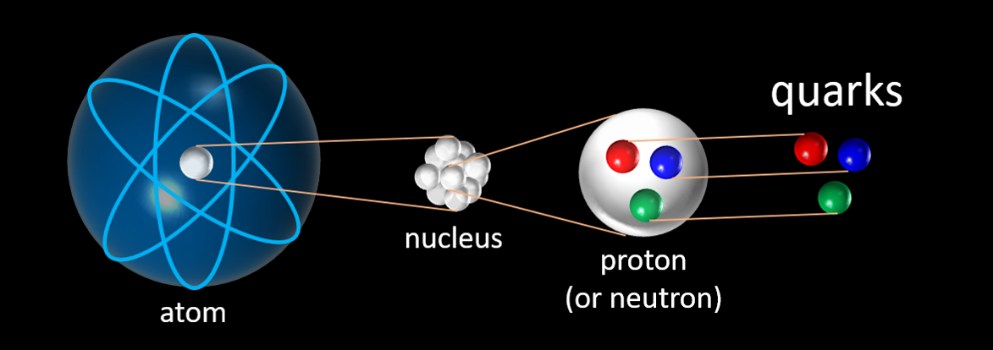
\includegraphics[width=\textwidth,keepaspectratio=true]{/Users/eparrish/Work/thesis/chapters/chapter2_theory/images/Atom_to_Quark_Cartoon.png}
        \caption{\tiny\cite{atom-to-quark} \cite{SM-Diagram}}
        % 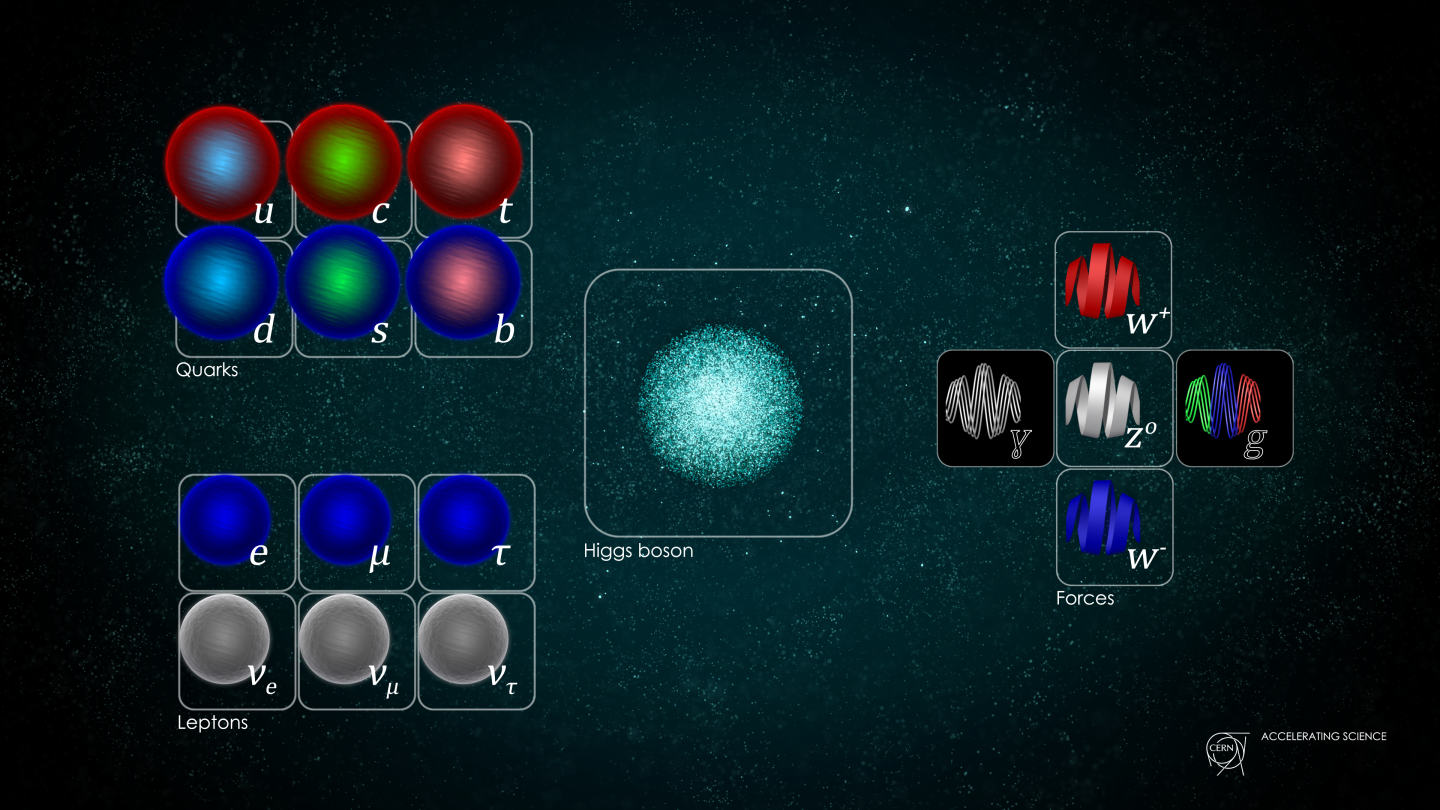
\includegraphics[width=\textwidth,keepaspectratio=true]{STDM higgs and field D.png}
        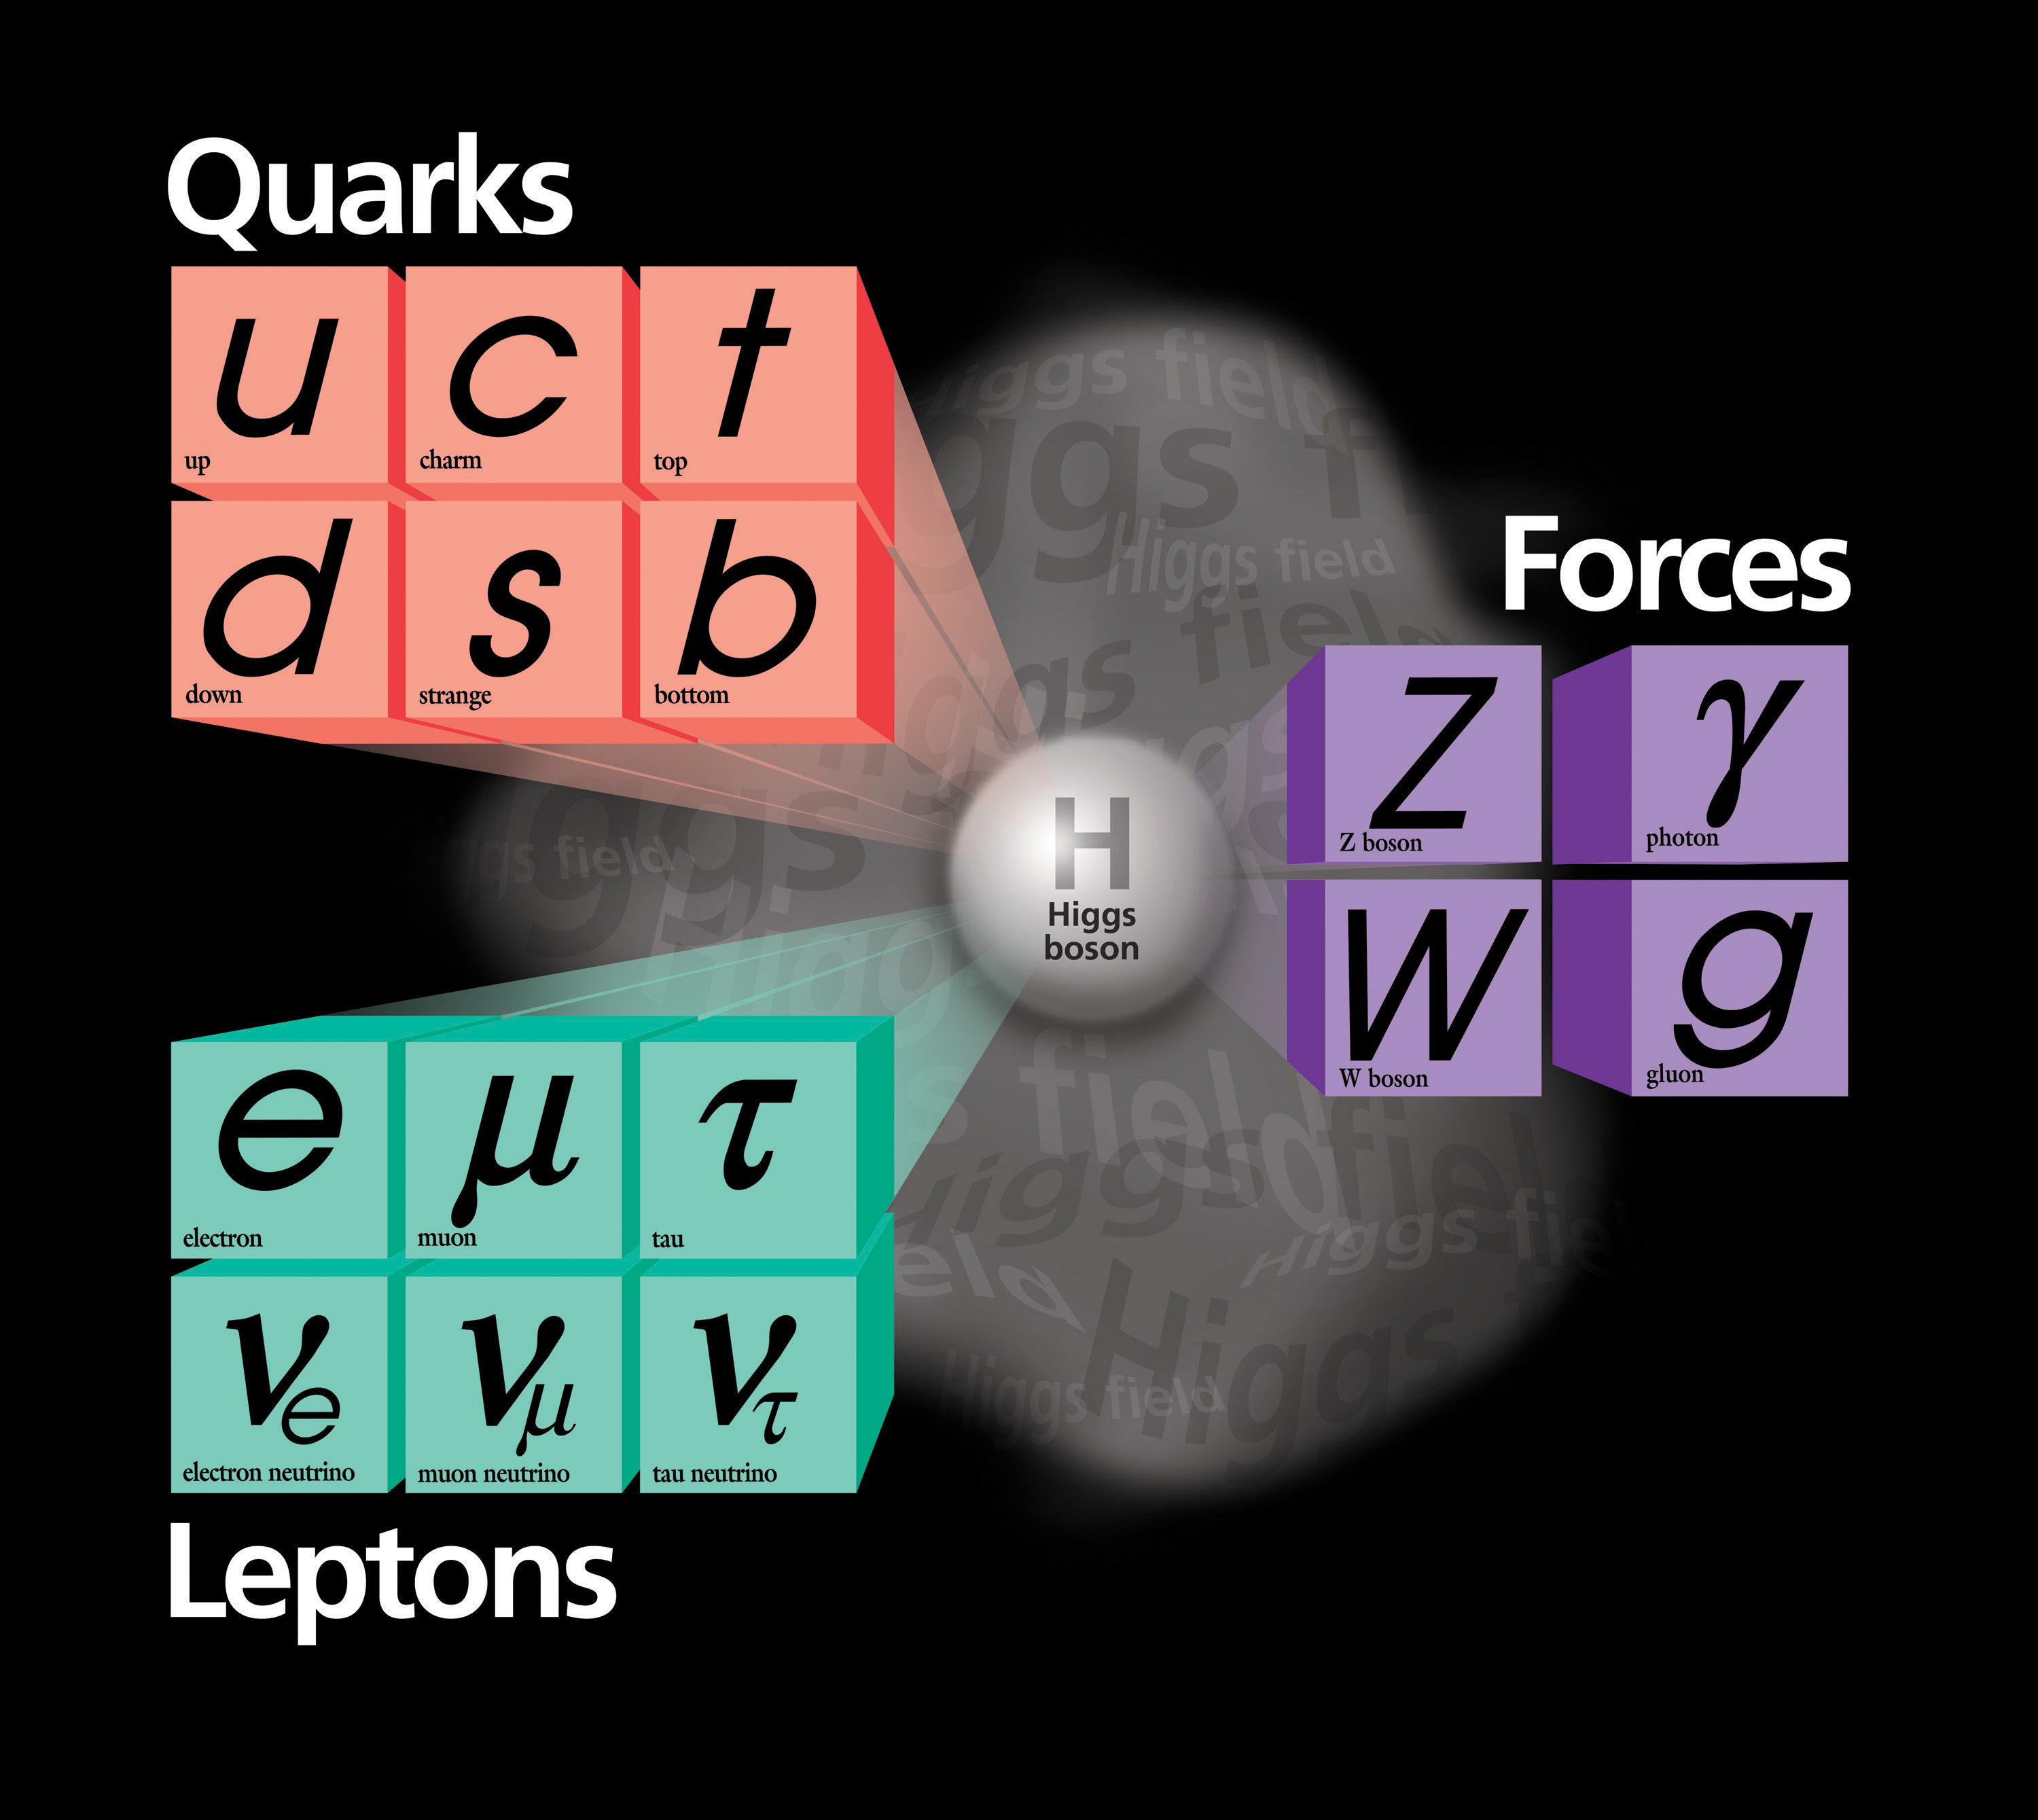
\includegraphics[height=.4\textheight,keepaspectratio=true]{SM High Res.jpeg}
      \end{figure}
    \end{columns}
  \end{frame}

  % \subsection{Higgs Boson}

  \begin{frame}[t]{The Higgs Boson}
    \begin{columns}[t]
    \column{.6\textwidth}
      \begin{itemize}
        % \item Interactions with Higgs field give particles mass
        % \item Theorized by Higgs, Englert, and Brout in 1964
          % \begin{itemize}
            \item At high energies, electromagnetism and the weak forces are one ``electroweak'' force
            \item Higgs field exists everywhere in space
            \begin{itemize}
              \item Non-zero vacuum expectation value
              \begin{itemize}
                \item This gives us electroweak symmetry breaking
              \end{itemize}
            \end{itemize}
            \item Interaction with Higgs field gives mass
            % \begin{itemize}
            % \item Complex scalar doublet
          % \end{itemize}
          % \end{itemize}
        \item Discovered jointly by the ATLAS and CMS collaborations in 2012
        % \item Why only one Higgs potential?
      \end{itemize}
    \column{.4\textwidth}
      % \vspace{-.80cm}
      \centering
      \begin{figure}
        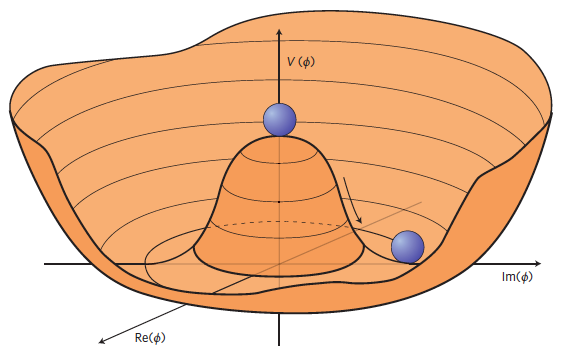
\includegraphics[height=.2\textheight,keepaspectratio=true]{/Users/eparrish/Work/thesis/chapters/chapter2_theory/images/higgspotential.png}
        \caption{\tiny \cite{Higgs-phys}}
      \end{figure}
      \begin{figure}
        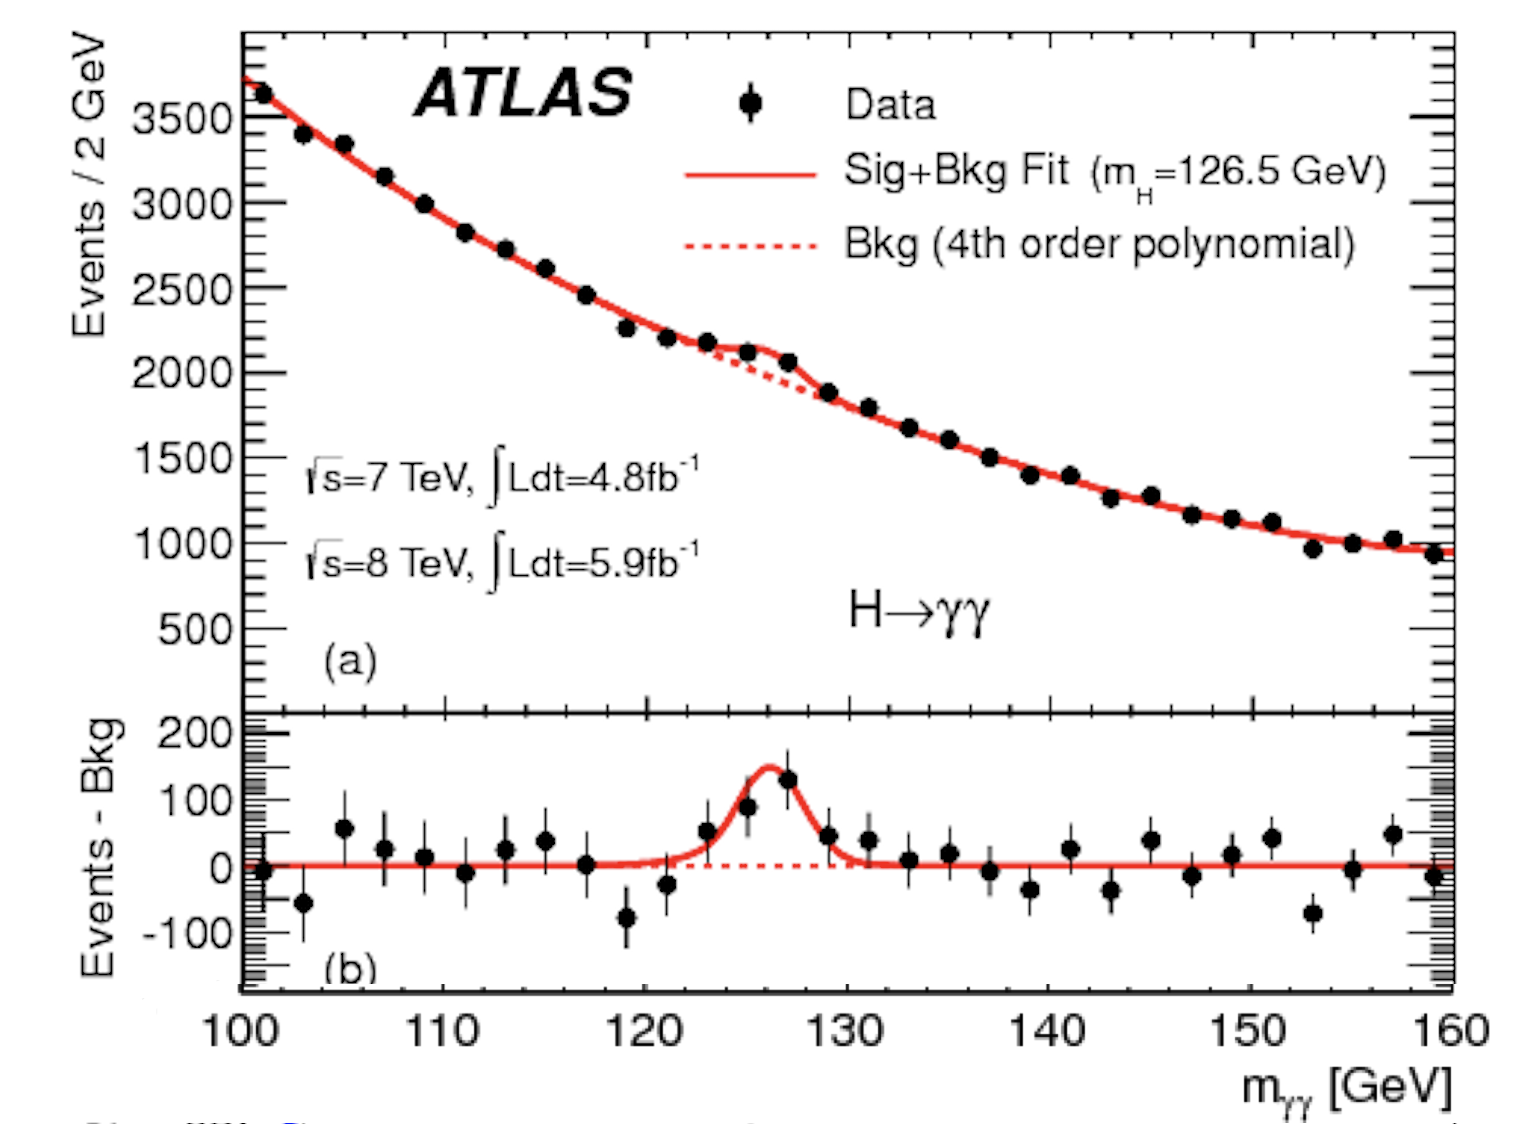
\includegraphics[height=.3\textheight,keepaspectratio=true]{/Users/eparrish/Work/thesis/chapters/chapter2_theory/images/Higgs_Discovery_gam_gam.png}
        \caption{\tiny \cite{higgs-discovery-atlas}}
      \end{figure}
    \end{columns}
  \end{frame}

  \begin{frame}[c]{The Standard Model}
    \begin{columns}
    \column{.45\textwidth}
      \small
      \begin{itemize}
        % \item Quantum field theory that explains the fundamental forces, particles, and their interactions
        \item Predicts the probabilities of creation and decay of particles (among many other things)
        \begin{itemize}
          \item Has been thoroughly tested
          \item Measurements agree to a high degree of accuracy
        \end{itemize}
        \item Not a complete theory ({\footnotesize Not a full list})
        \begin{itemize}
          \item Gravity
          \item Matter-antimatter asymmetry in the universe
          \item Hierarchy problem
            \begin{itemize}
          %     % \item Large Higgs mass terms cancel to give $\sim 125$ GeV
              \item EW scale is $\sim 100$ GeV
              \item Planck scale is $\sim 10^{18}$ GeV
          %     % \item Supersymmetry (SUSY) offers many new particles to occupy the intermediate range
            \end{itemize}
          % \item Predicted neutrino masses are 0
          % \begin{itemize}
          %   \item Observed neutrino mixing says otherwise
          % \end{itemize}
          % \item 
        \end{itemize}
      \end{itemize}
    \column{.55\textwidth}
      \begin{figure}
        \centering
        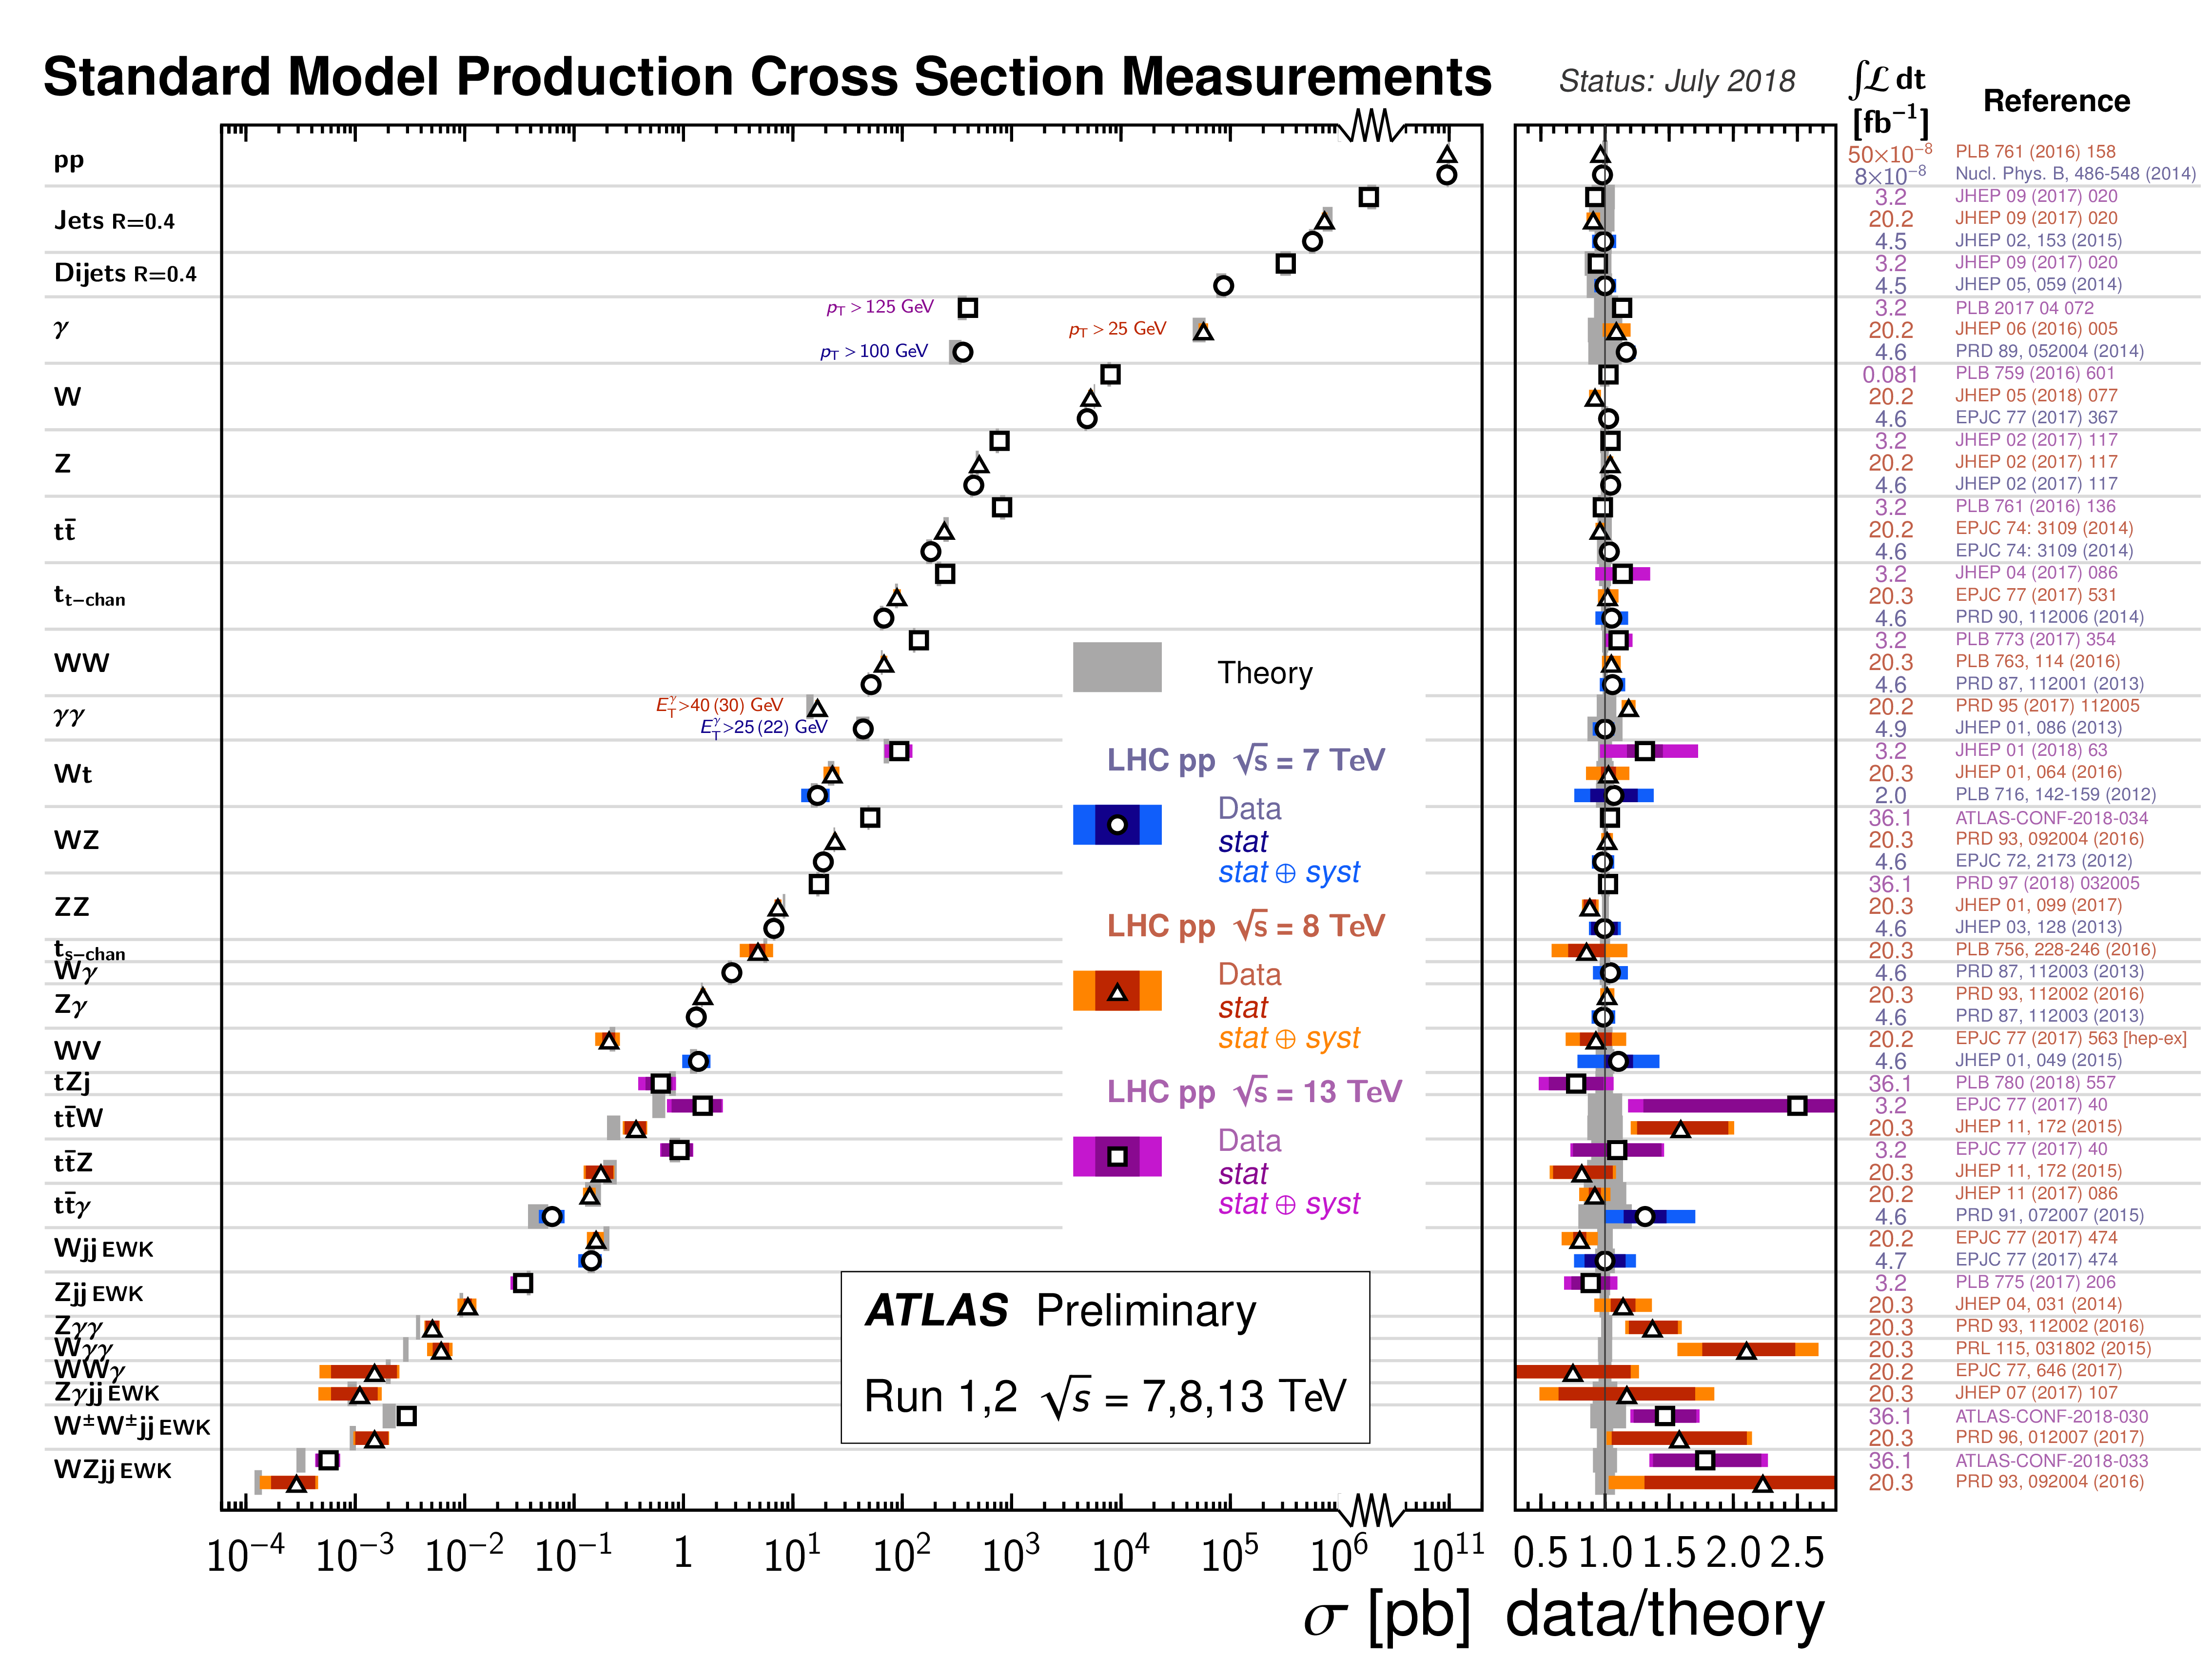
\includegraphics[width=\textwidth,keepaspectratio=true]{ATLAS_d_SMSummary_FiducialXsect_rotated.png}
        % \caption{\tiny}
      \end{figure}
    \end{columns}
  \end{frame}

  \subsection{New Physics }

    \begin{frame}[t]{Beyond the Standard Model}
      \begin{columns}[t]
      \column{.8\textwidth}
        \begin{itemize}
        %   \item Hierarchy problem, ``unnaturalness''
        %   \begin{itemize}
        %     % \item Large Higgs mass terms cancel to give $\sim 125$ GeV
        %     \item Electroweak scale is $\sim 100$ GeV
        %     \item Planck scale is $\sim 2.4 \times 10^{18}$ GeV
        %     % \item Supersymmetry (SUSY) offers many new particles to occupy the intermediate range
        %   \end{itemize}
          % \item SUSY proposes a symmetry between fermions and bosons (spin)
          % \begin{itemize}
          %   \item $Fermion \Rightarrow Boson$ 
          %   \item $Boson \Rightarrow Fermion$
          % \end{itemize}
          \item 2 Higgs Doublet Models and Supersymmetry (SUSY) are large groups of theories attempting to address these issues
          \begin{itemize}
            \item 2HDM have two complex doublet scalar fields \cite{2HDM}
            \begin{itemize}
              \item Two relevant free parameters, \tanb and \mHpm
              \item \tanb is the ratio of the vacuum expectation values of the two doublets
            \end{itemize}
            \item SUSY proposes a symmetry between fermions and bosons
              \begin{itemize}
                \item Many new possible particles
                \item Minimal Supersymmetric Standard Model (MSSM) is the smallest SUSY extension to the SM
              \end{itemize}
          \end{itemize}
        \end{itemize}
      \column{.2\textwidth}
      \begin{centering}
      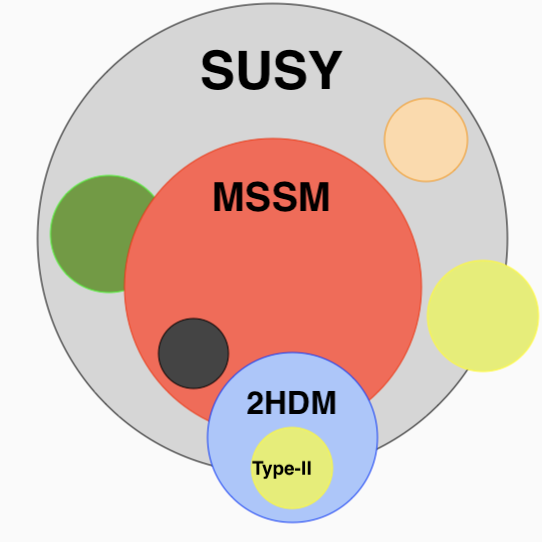
\includegraphics[height=.4\textheight,keepaspectratio=true]{SUSY_Bubble.png}
      \end{centering}
      \centering
        \begin{table}[!thp]
          \centering
          \resizebox{\textwidth}{!}{
          \rowcolors{1}{}{NIUgray}
          \begin{tabular}{| l | c |}
          \hline
          light neutral scalar  & $h^0$ \\ \hline
          heavy neutral scalar  & $H^0$ \\ \hline
          neutral pseudoscalar  & $A^0$ \\ \hline
          two charged scalars   & \Hpm \\ \hline
          % \boxit{1.75in} 
          \end{tabular}}
          % \caption{\cite{2HDM}}
      \end{table}
      \end{columns}
    \end{frame}

  \subsection{Charged Higgs Bosons }

    \begin{frame}[t]{Charged Higgs Bosons}
      \begin{columns}
      \column{.75\textwidth}
      \begin{itemize}
        % \item Many extensions to the Higgs sector imply the existence of charged scalars (2HDM, NMSMM, Triplet, etc.)
        % \begin{itemize}
          % \begin{itemize}
          %   \item $\mathrm{tan} \beta$ defined as the ratio of the  vacuum expectation values of the two doublets
          % \end{itemize}
        % \end{itemize}
        \item At the LHC, theoretical production mode of \mHpm is mainly in top-quark decays or in association with a top-quark ($t$)
        \begin{itemize}
          \item $H^{\pm}$ production mode is dependent on \mHpm
          % \item Analysis is sensitive for low mass $(\mHpm < m_{t})$, intermediate mass $(\mHpm \simeq m_{t})$, and high mass $(\mHpm > m_{t})$
        \end{itemize}
        \begin{columns}
          \column{.3\textwidth}
            \begin{figure}
              \tiny
              \fcolorbox{black}{white}{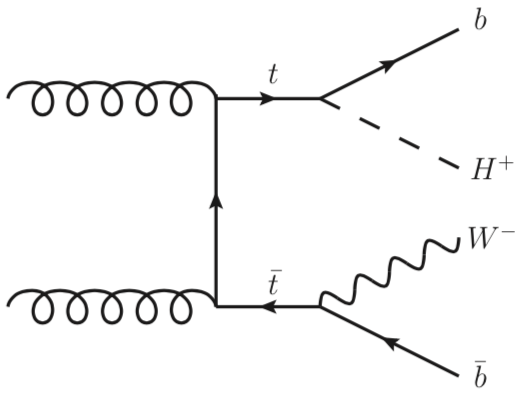
\includegraphics[width=.72\textwidth,keepaspectratio=true]{double_resonant_production_low_mass.png}}
              \caption{$\mHpm < m_{t}$}
            \end{figure}
          \column{.3\textwidth}
            \begin{figure}
              \tiny
              \fcolorbox{black}{white}{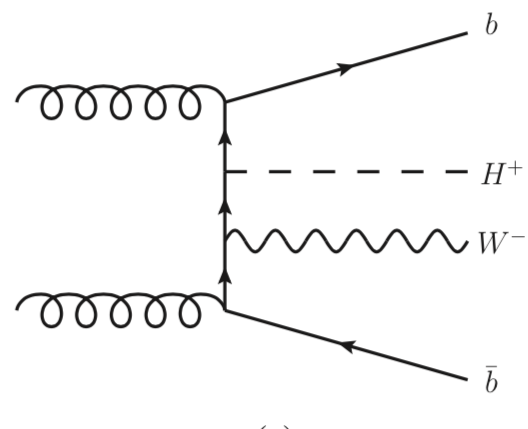
\includegraphics[width=.72\textwidth,keepaspectratio=true]{non_resonant_production_intermediate_mass.png}}
              \caption{$\mHpm \simeq m_{t}$}
            \end{figure}
          \column{.3\textwidth}
            \begin{figure}
              \tiny
              \fcolorbox{black}{white}{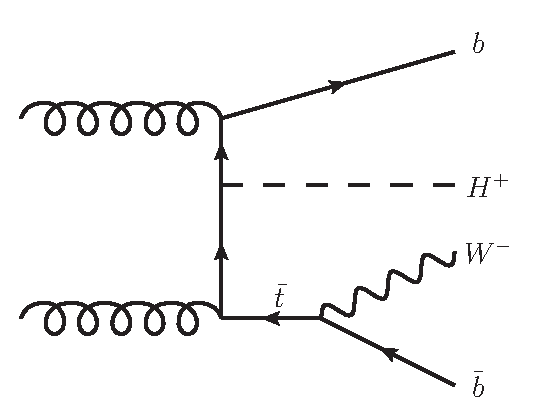
\includegraphics[width=.72\textwidth,keepaspectratio=true]{SingleResonant.pdf}}
              \caption{$\mHpm > m_{t}$}
            \end{figure}
        \end{columns}
        \item \HpmLong decay channel remains significant for high \tanb
        \item Two sub-channels based on the decay mode of associated $t$ 
        % \begin{itemize}
        %   \item $t \rightarrow jets$ 
        %     \begin{itemize}
        %       \item Sensitive at high mass due to higher $W \rightarrow q\bar{q}$ BR
        %     \end{itemize}
        %     \item $t \rightarrow \ell$
        %     \begin{itemize}
        %       \item Sensitive at low mass due to single lepton triggers
        %     \end{itemize}
        % \end{itemize}
      \end{itemize}

      \vspace{-.3cm}
      \centering
      \begin{table}
          % \small
          \resizebox{.9\textwidth}{!}{
          \rowcolors{1}{}{NIUgray}
          \begin{tabular}{c | c}
          \textbf{$t \to Wb \to jets$ } & $t \to Wb \to \ell$ \\
          \hline \hline
          Sensitive at high mass due to higher $W \to q\bar{q}$ BR & Sensitive at low mass due to easier triggering \\
          \end{tabular}}
        \end{table}

      \column{.25\textwidth}
      \centering
      % 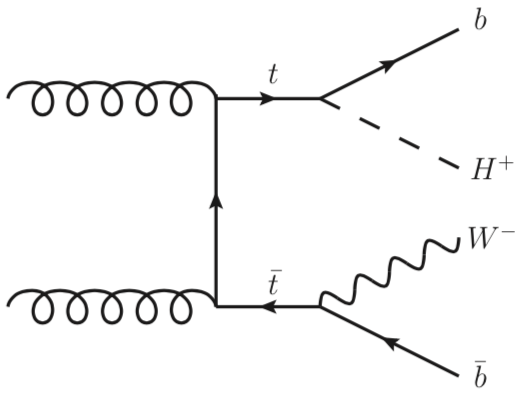
\includegraphics[width=.74\textwidth,keepaspectratio=true]{double_resonant_production_low_mass.png}
      % 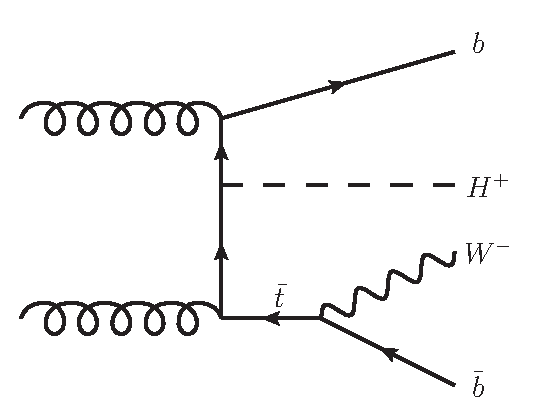
\includegraphics[width=.74\textwidth,keepaspectratio=true]{SingleResonant.pdf}
      % 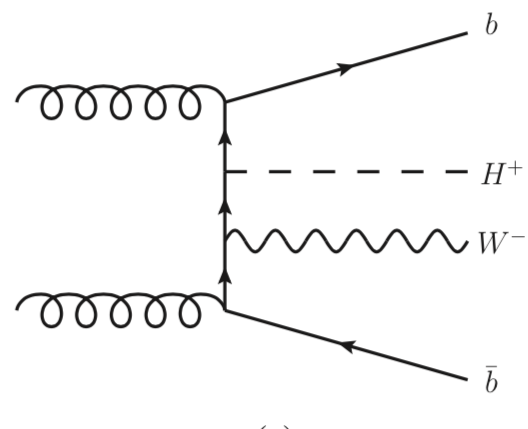
\includegraphics[width=.74\textwidth,keepaspectratio=true]{non_resonant_production_intermediate_mass.png}
      % 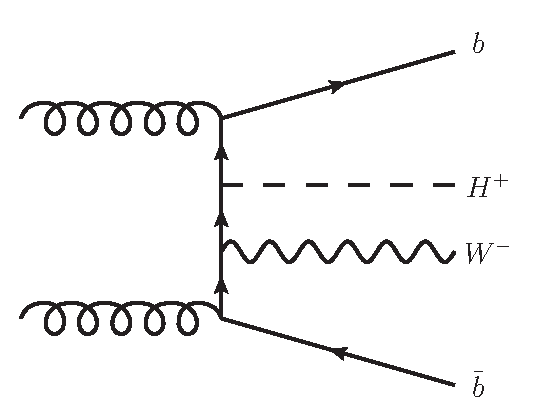
\includegraphics[width=.74\textwidth,keepaspectratio=true]{NonResonant.pdf}
      % 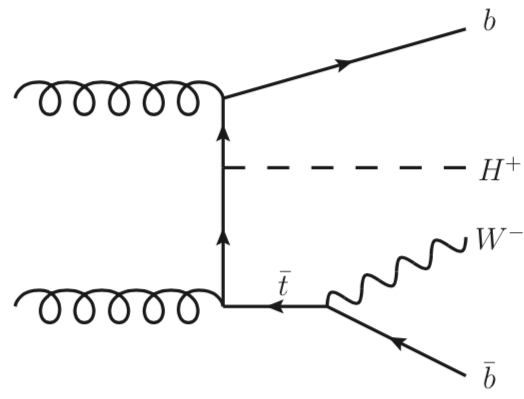
\includegraphics[width=.74\textwidth,keepaspectratio=true]{single_resonant_production_large_mass.png}
      % 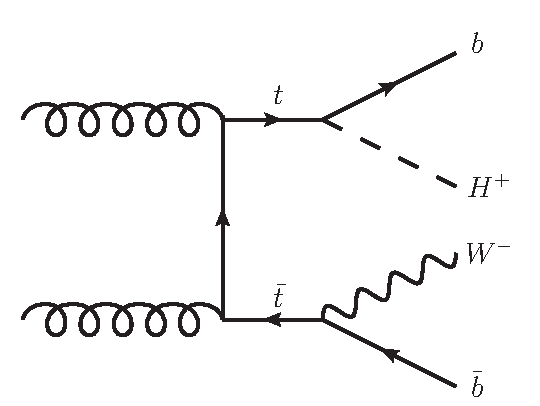
\includegraphics[width=.74\textwidth,keepaspectratio=true]{DoubleResonant.pdf}
      % 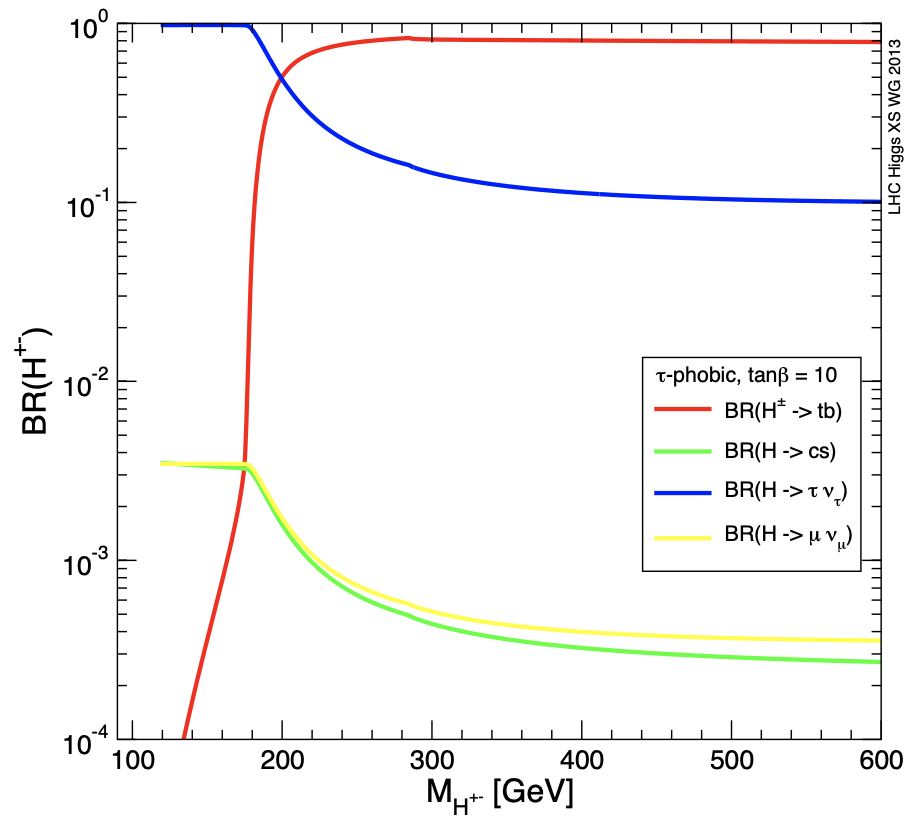
\includegraphics[width=1.15\linewidth,keepaspectratio=true]{Charged_Higgs_BR.png}
      \begin{figure}
      \begin{columns}
      \column{.95\textwidth}
      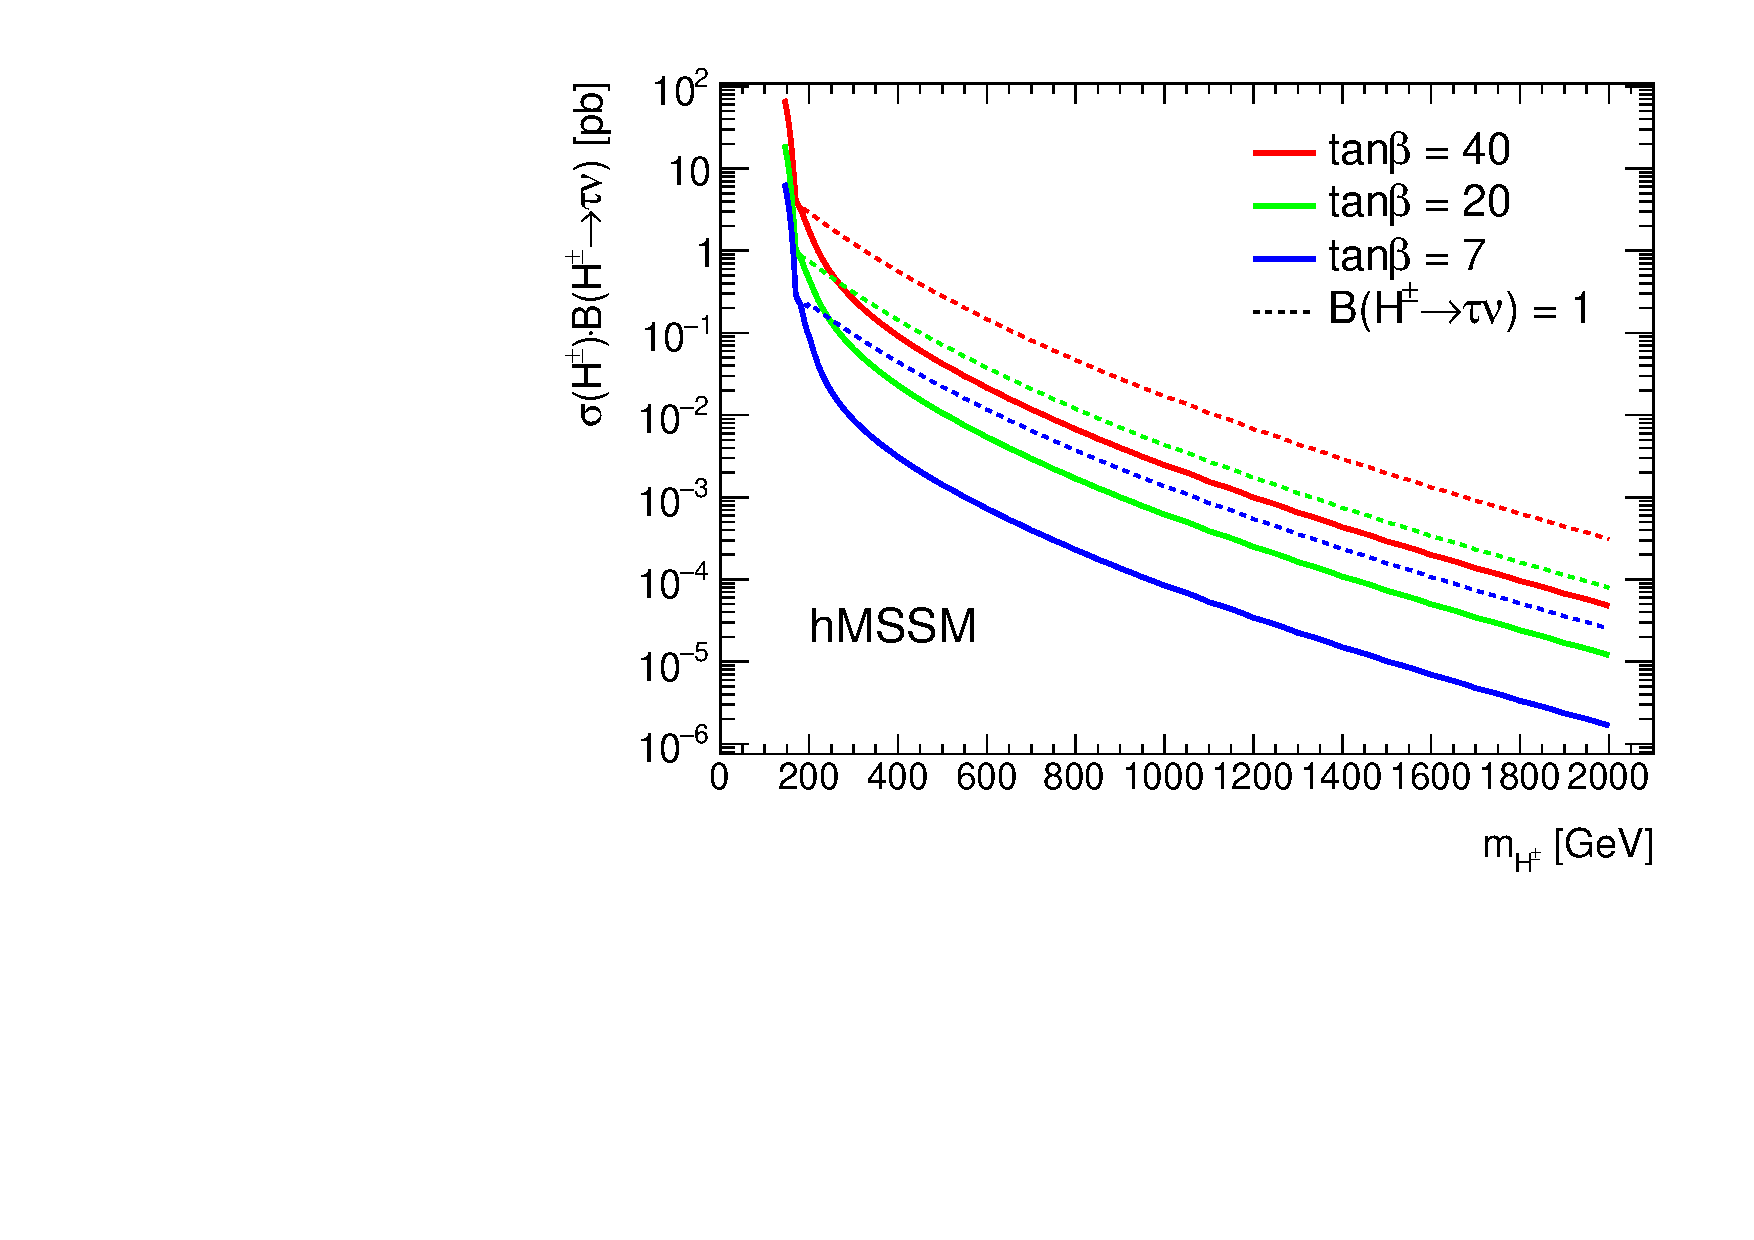
\includegraphics[width=1\textwidth,keepaspectratio=true]{/Users/eparrish/Work/thesis/chapters/chapter2_theory/images/XSBR_hmssm.pdf}
      \column{.05\textwidth}
      \caption{\tiny \cite{hpm-previous}}
      \end{columns}
      \end{figure}
      \begin{figure}
      \begin{columns}
      \column{.95\textwidth}
      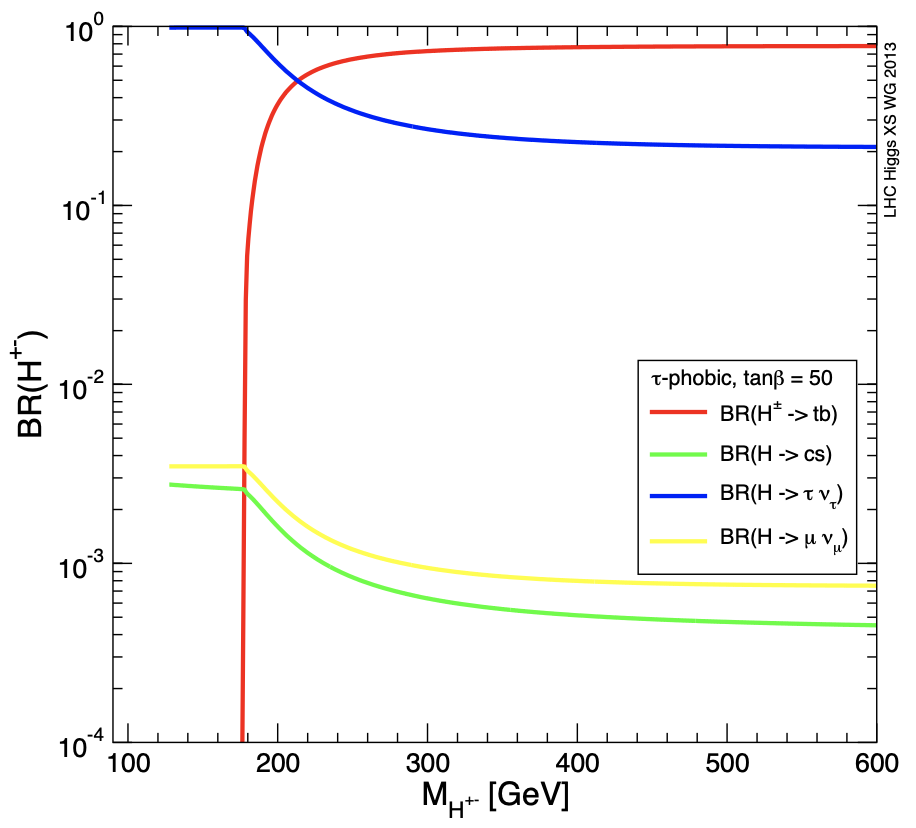
\includegraphics[width=1\textwidth,keepaspectratio=true]{HPlus_taunu_tanB.png}
      \column{.05\textwidth}
      \caption{\tiny \cite{Higgs-Crosssections}}
      \end{columns}
      \end{figure}
      \end{columns}
    \end{frame} 

    \begin{frame}{\href{https://link.springer.com/article/10.1007/JHEP09(2018)139}{\textcolor{blue}{JHEP 09(2018)139}} Limits on charged Higgs bosons}
      \begin{columns}
        \column{.5\textwidth}
        \centering
        \begin{itemize}
          \item Previous limits on the production of \HpmLong and the free parameters \tanb and \mHpm
        \end{itemize}
        % 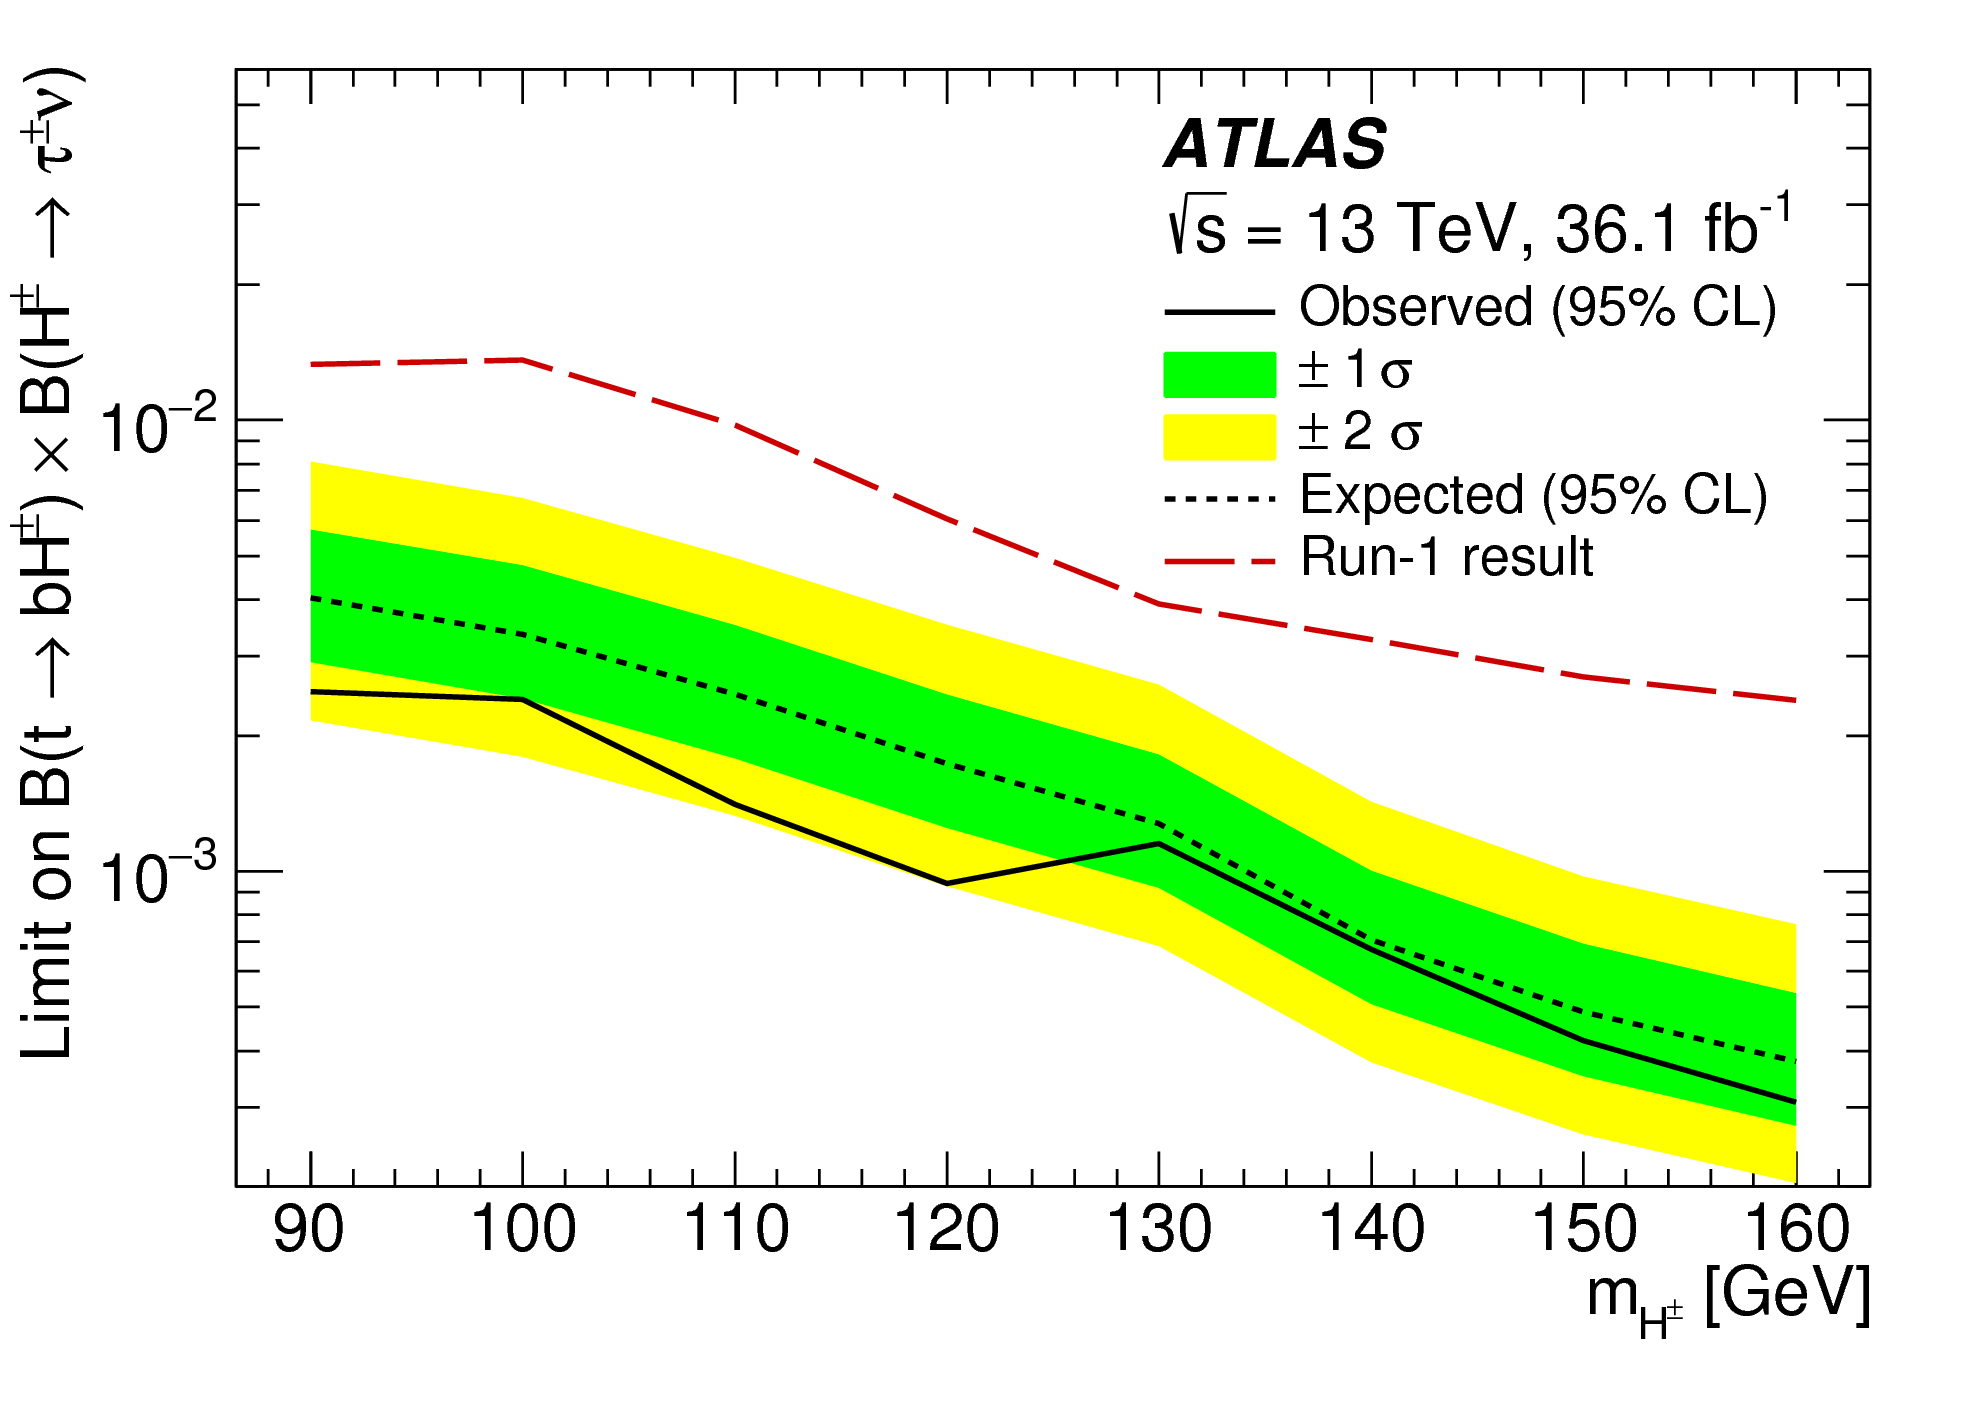
\includegraphics[width=.65\textwidth,keepaspectratio=true]{Limits/Combined_low_NoLabel_2018.png}
        % \column{.25\textwidth}
        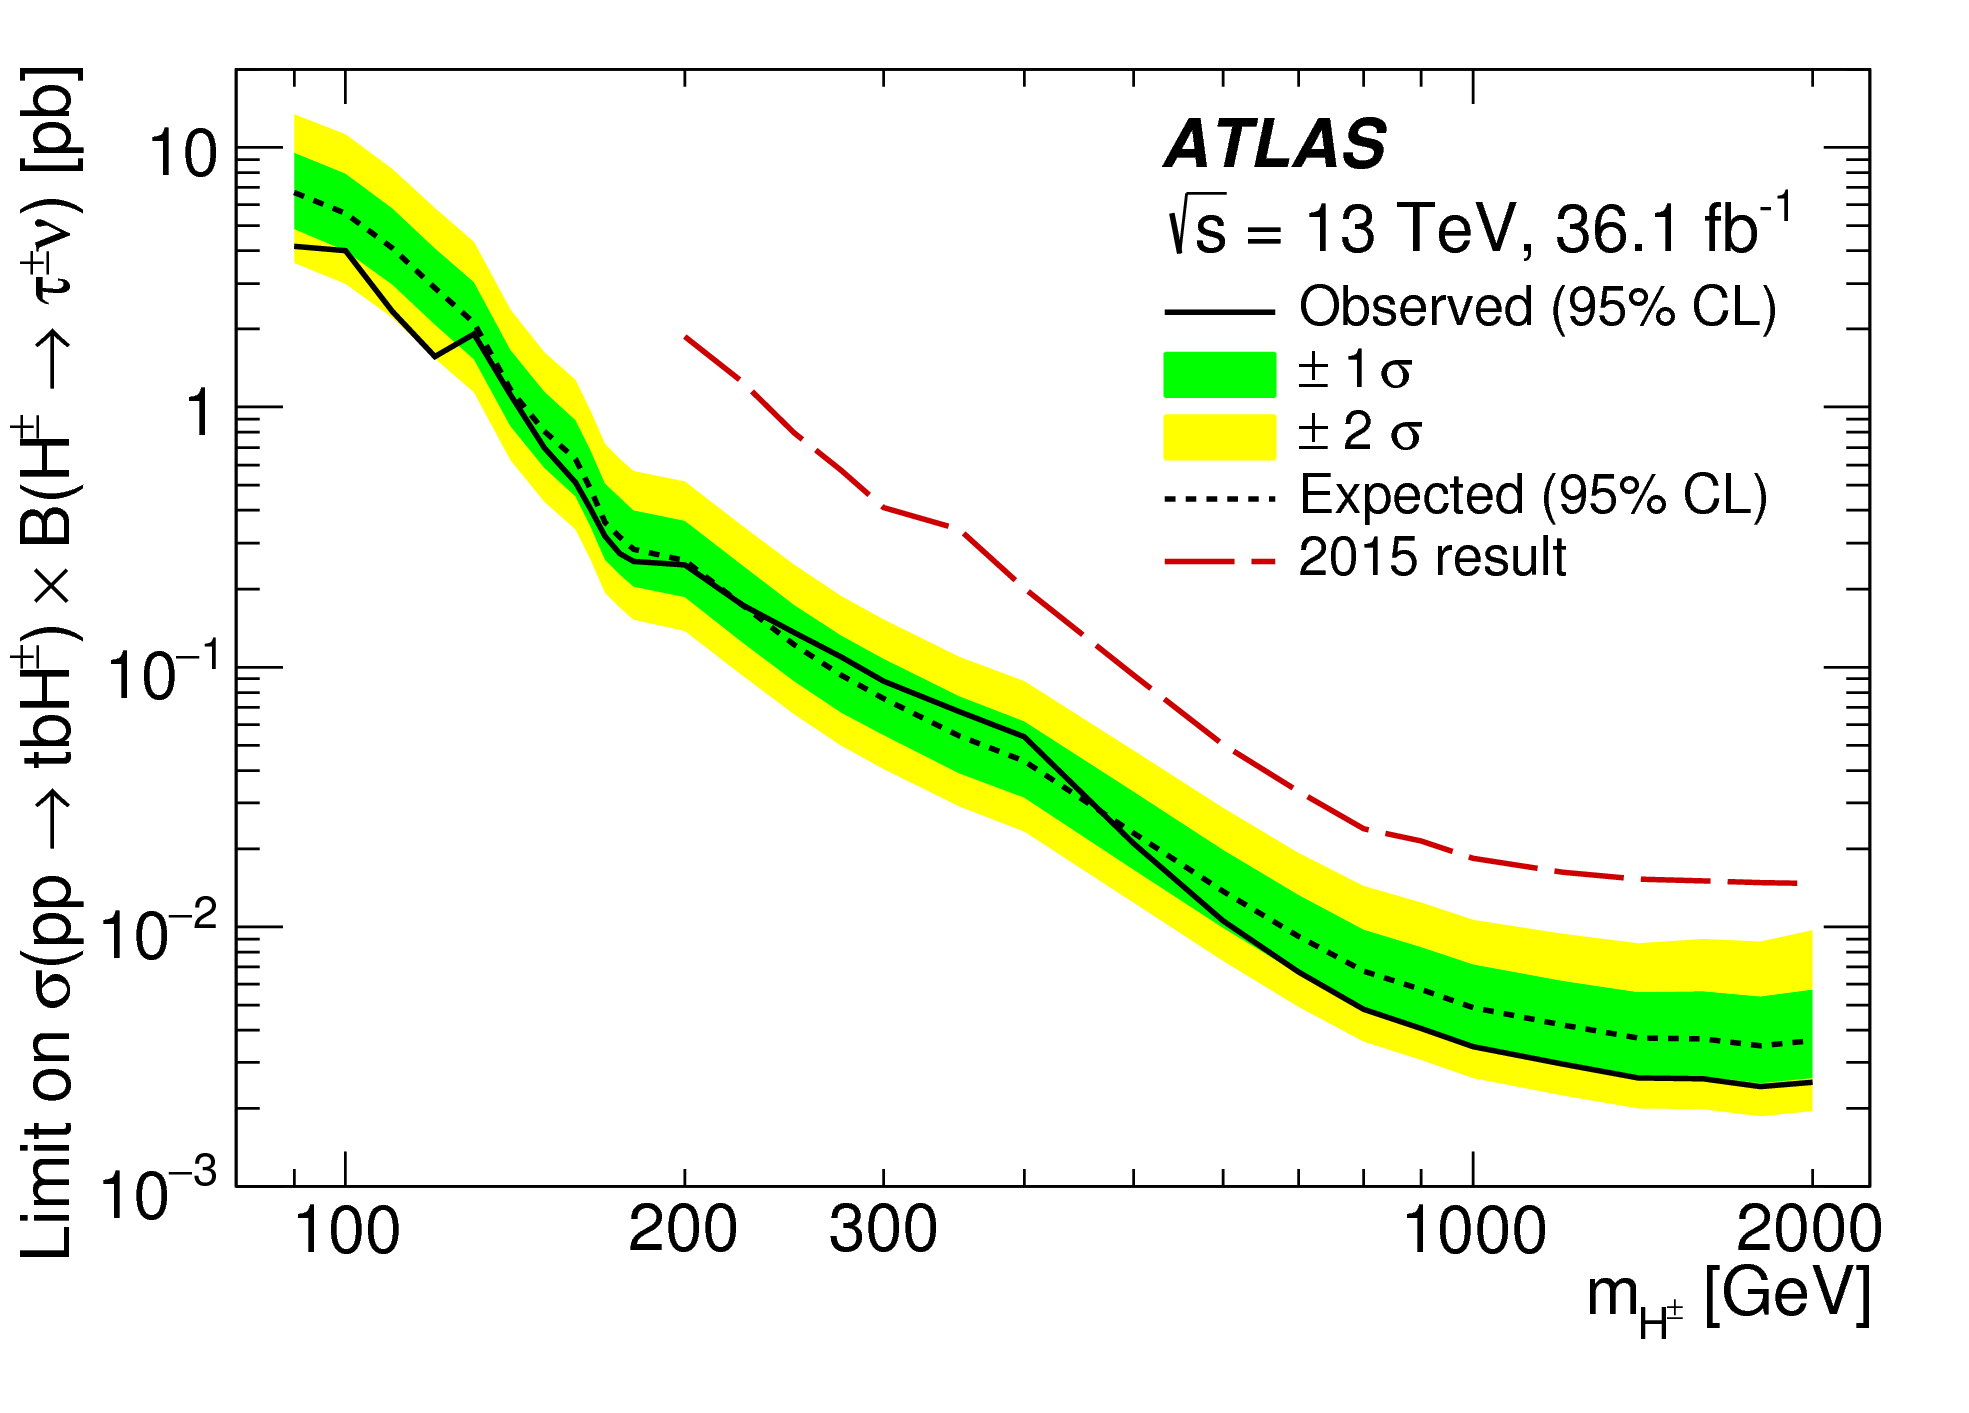
\includegraphics[width=\textwidth,keepaspectratio=true]{Limits/Combined_CrossSection_2018.png}
        \column{.5\textwidth}
        \centering
        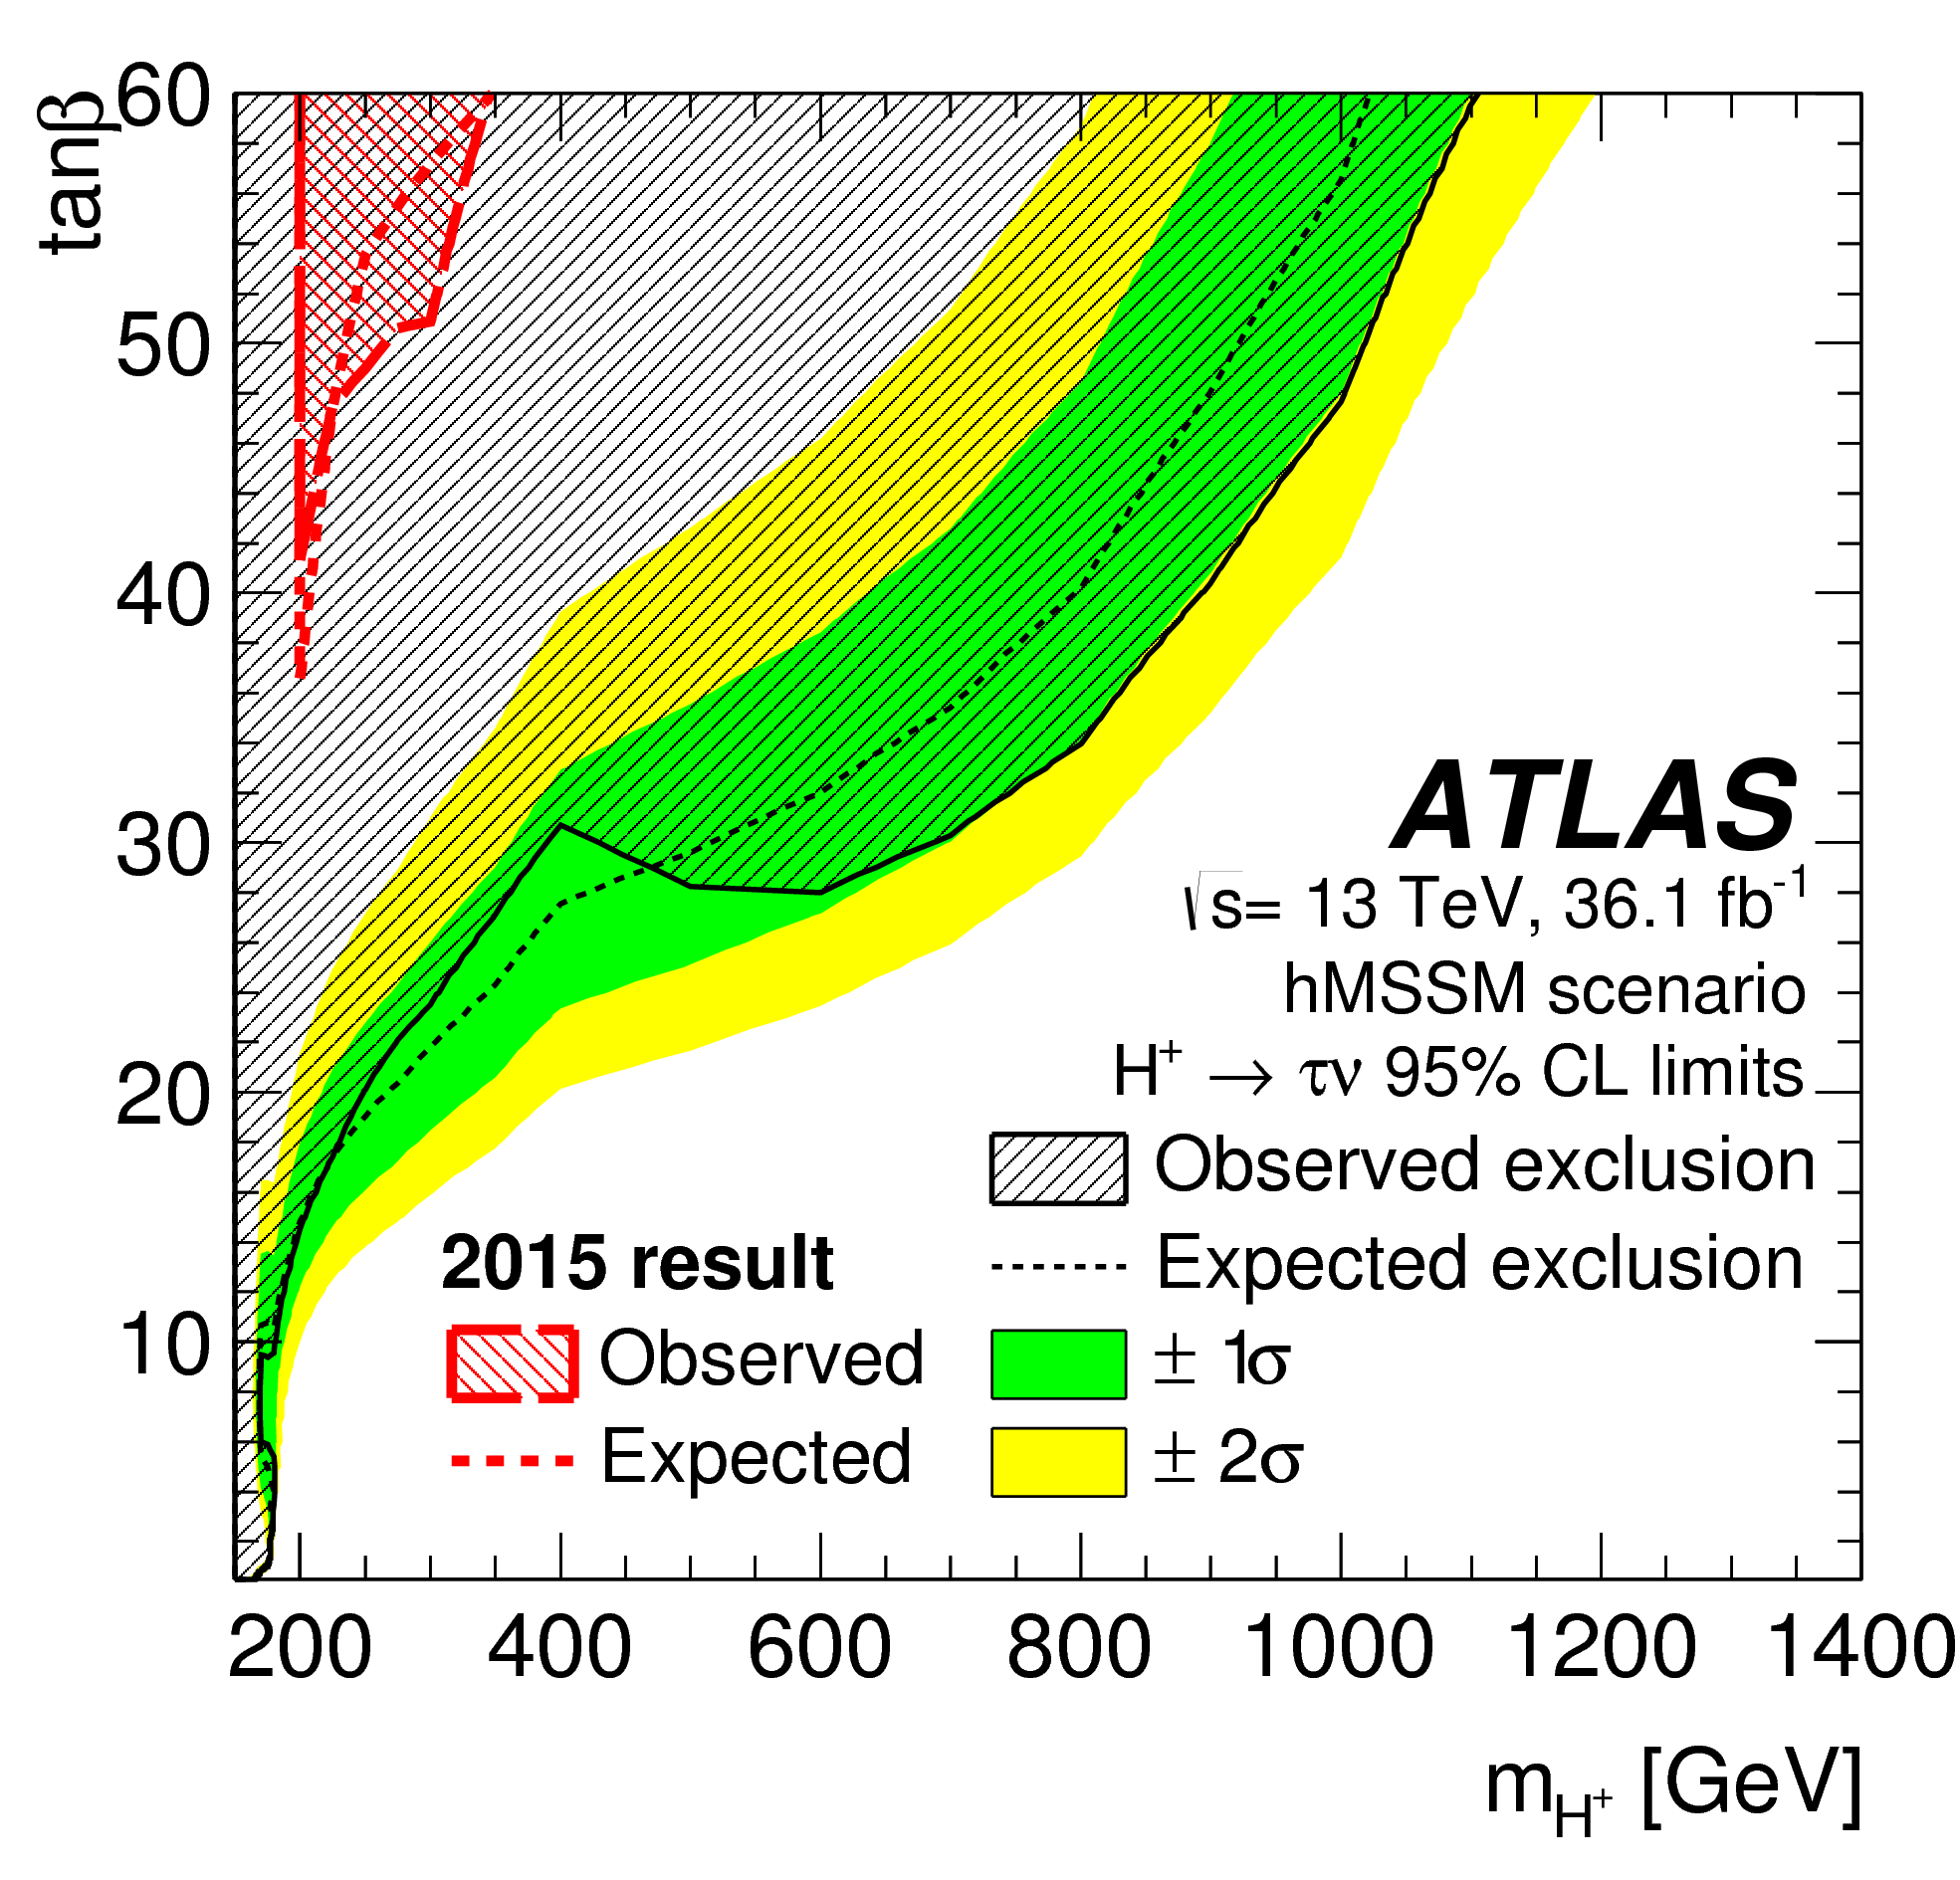
\includegraphics[width=\textwidth,keepaspectratio=true]{Limits/tanB_Limit_2018.png}
      \end{columns}
    \end{frame}

    \begin{frame}[t]{Other \Hpm Searches}
    \begin{columns}
    \column{.5\textwidth} 
      \centering
      \begin{figure}
      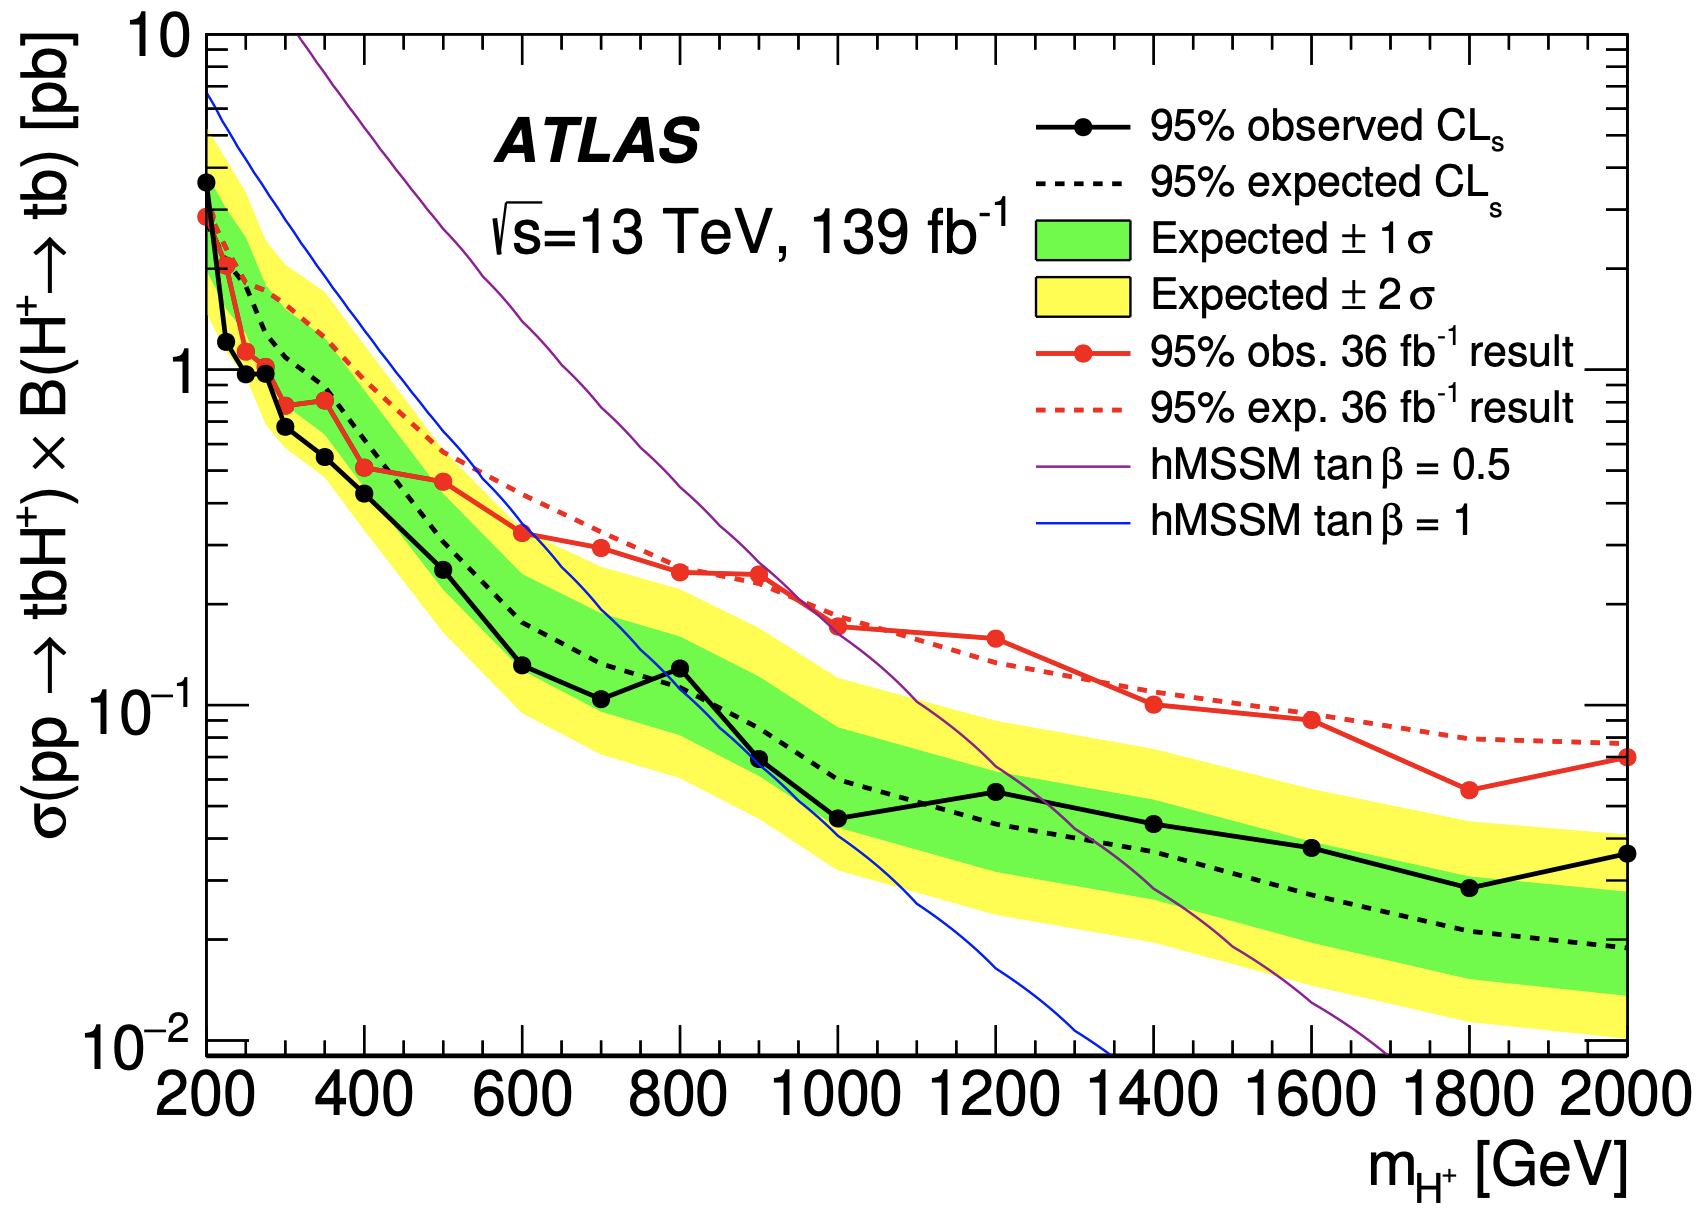
\includegraphics[width=\textwidth,keepaspectratio=true]{/Users/eparrish/Work/thesis/chapters/chapter2_theory/images/HPlus_to_tb_Limits.png}
      \caption{\tiny \cite{Hpm-to-tb} }
      \end{figure}
    \column{.5\textwidth} 
      \centering
      \begin{figure}
      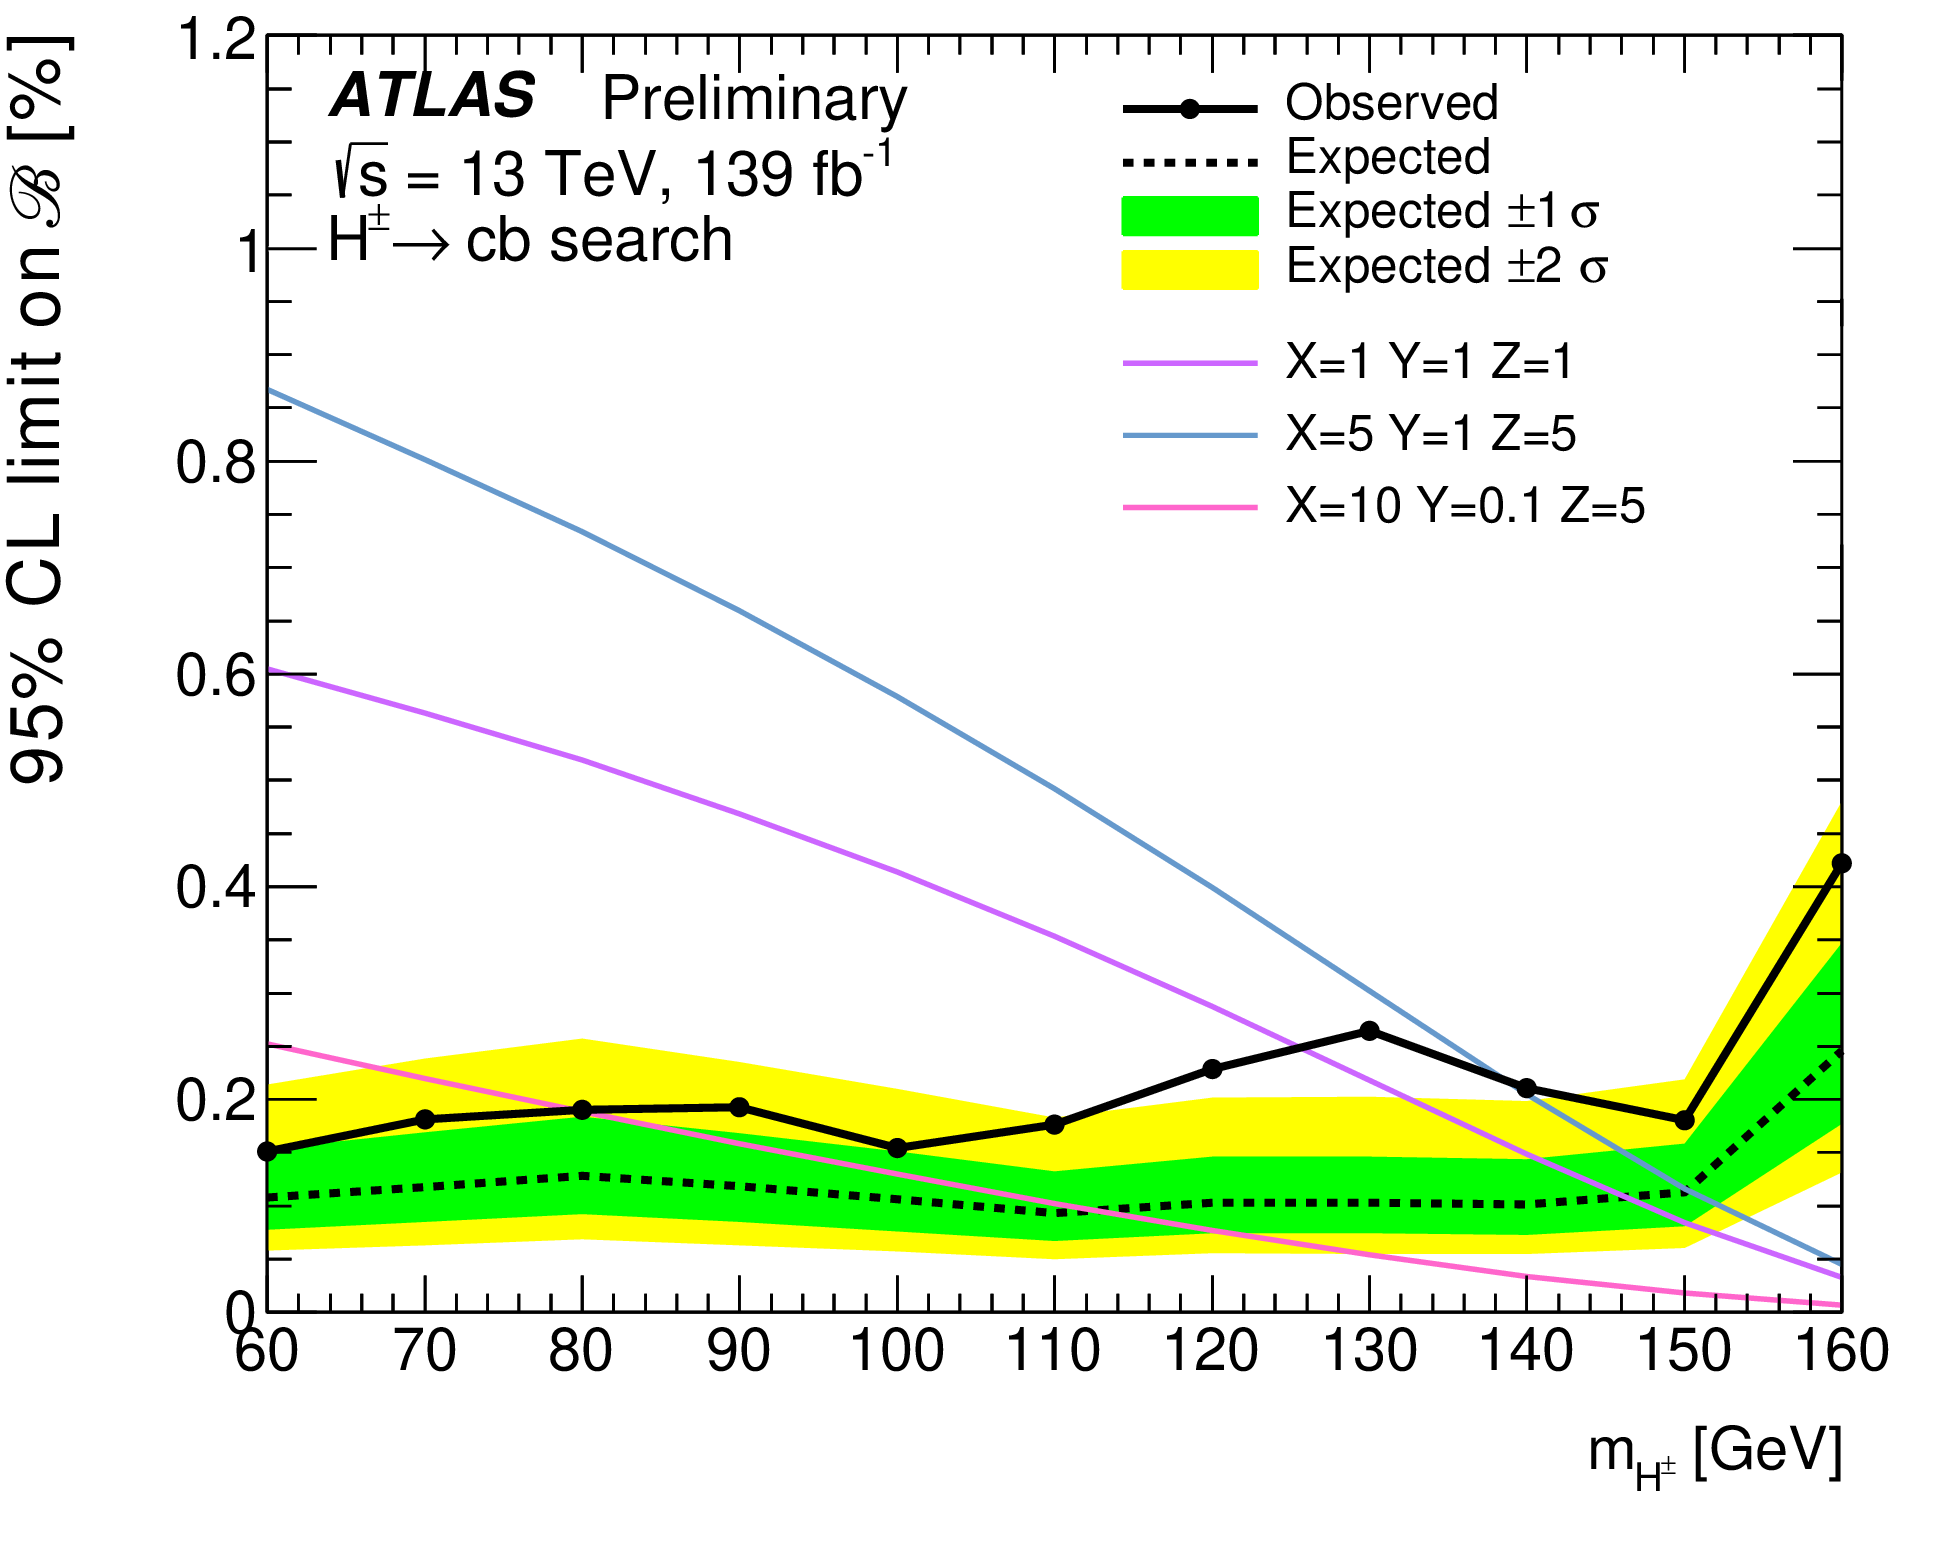
\includegraphics[width=\textwidth,keepaspectratio=true]{/Users/eparrish/Work/thesis/chapters/chapter2_theory/images/HPlus_to_cb_Limits.png}
      \caption{\tiny \cite{Hpm-to-cb} }
      \end{figure}
    \end{columns}
    \end{frame}

\section{Experimental Apparatus }

  \begin{frame}[t]{Particle Collisions}
    \begin{columns}[t]
      \column{.5\textwidth}
        \begin{itemize}
          \item Most particles we are interested in are not stable and cannot be observed in our environment
          \item Collide known particles to study them and potentially new particles
            \begin{itemize}
              \item $E^2 = m^2c^4 + p^2c^2$
            \end{itemize}
          \item Hadronization
          \begin{itemize}
            \item Quarks cannot exist on their own
            \item Must combine to form bound states
            \item Combine shower into a \textit{jet}
          \end{itemize}
        \end{itemize}

      \column{.5\textwidth}
        \begin{figure}
        \centering
        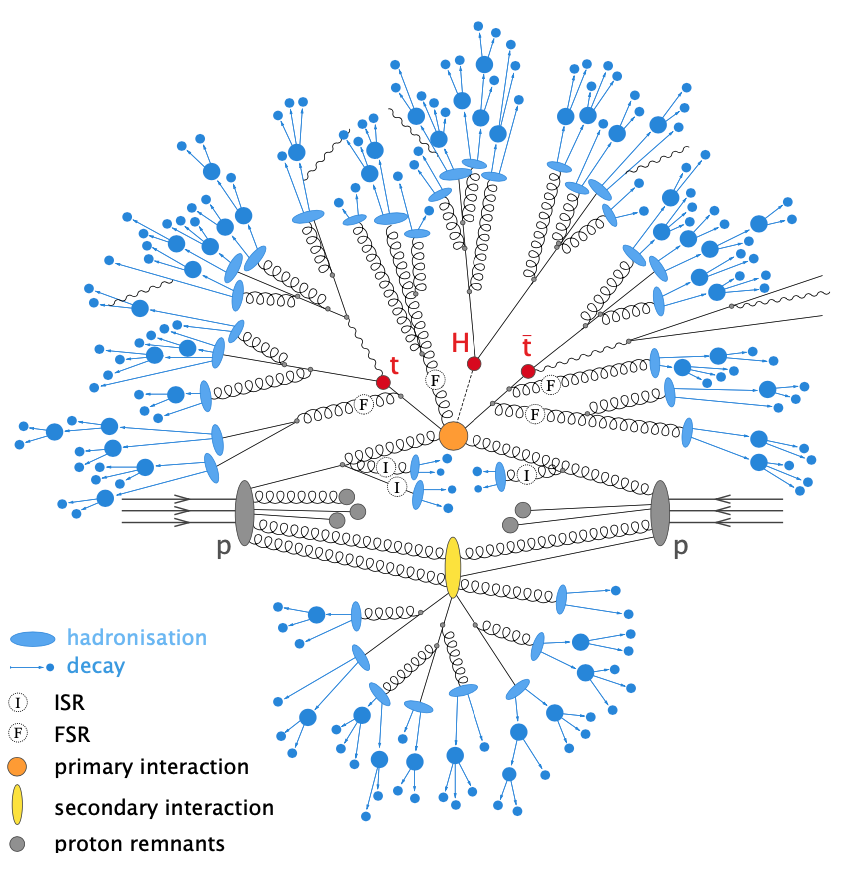
\includegraphics[width=.8\textwidth,keepaspectratio=true]{/Users/eparrish/Work/thesis/chapters/chapter4_simulation/images/tth_hadronization_gen.png}
        \caption{\tiny \cite{Wanotayaroj:2242196}}
        \end{figure}

    \end{columns}
  \end{frame}

  \subsection{LHC }

    \begin{frame}[t]{Large Hadron Collider}
      \begin{columns}[t]
        \column{.5\textwidth}
          \begin{itemize}
            \item Largest particle collider ever built
            \item Highest energy particle collider
              % \begin{itemize}
              %   \item Center of mass energy of 13 TeV
              % \end{itemize}
            \item Located at CERN outside of Geneva, Switzerland
            \item Four main collision points
            \begin{itemize}
              \item \textbf{ATLAS}, ALICE, CMS, LHCb
            \end{itemize}
          \end{itemize}
          \centering

          \begin{table}[!thp]
            \begin{columns}
            \column{.95\textwidth}
            \centering
            \resizebox{\textwidth}{!}{
            \rowcolors{1}{}{NIUgray}
            \begin{tabular}{| l | l |}  
            \multicolumn{2}{c}{\textbf{Selected Run-2 LHC Parameters}} \\ \hline \hline
            Circumference                   & $26,659$ m          \\  \hline
            Magnet operating temperature    & $1.9$ K             \\  \hline
            % Dipole magnets                & $1232$            \\  \hline
            % Quadrapole magnets            & $392$             \\  \hline
            % Radiofrequency cavities       & $16$ ($8$ per beam)       \\  \hline
            Beam energy                     & $6.5$ TeV ($13$ CM TeV)     \\ \hline
            Protons per bunch               & $1.2 \times 10^{11}$      \\ \hline
            Bunches per beam                & $2808$            \\ \hline
            % Revolutions per second        & $11245$             \\ \hline
            % Speed of bunches                & $>1 \times 10^9$ km/hr ($\simeq99.999\% \, c$) \\ \hline
            Speed of bunches                & $> 1,000,000,000$ km/hr ($\simeq99.999\% \, c$) \\ \hline
            % Collisions per second           & $1,000,000,000$         \\ \hline
            \end{tabular}}
            \column{.05\textwidth}
            \caption{\tiny \cite{lhc-facts}}
            \end{columns}
          \end{table}
          
        \column{.5\textwidth}
          \centering
          % \begin{figure}
          % 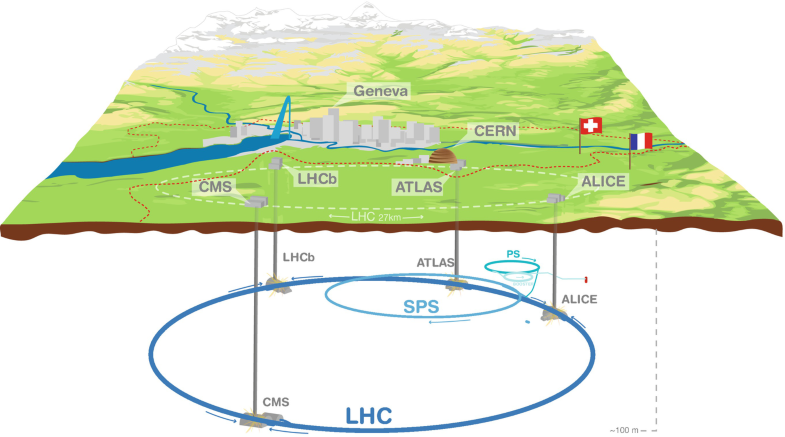
\includegraphics[width=.75\textwidth,keepaspectratio=true]{LHC.png}

          % \end{figure}

          \begin{figure}
          \begin{centering}
          \includegraphics[width=\textwidth,keepaspectratio=true]{/Users/eparrish/Work/thesis/chapters/chapter3_experiment/images/CERN-complex.png}
          \caption{\tiny \cite{CERN-complex}}
          \end{centering}
          \end{figure}

      \end{columns}
    \end{frame}

  \subsection{ATLAS }

    \begin{frame}[t]{The ATLAS Detector}
      \begin{columns}[t]
      \column{.4\textwidth}
        \begin{itemize}
          \item General purpose particle detector
            \begin{itemize}
              \item Magnet System
              \item Tracker
              \item Calorimeters
              \item Muon Spectrometer
            \end{itemize}
          \item Coordinate system origin at interaction point
          \begin{itemize}
            \item r is radial distance
            \item $\eta \equiv - \mathrm{ln}(\mathrm{tan}(\frac{\theta}{2}))$
            \item $\phi$ is azimuthal angle
          \end{itemize}
          % \item Complex machine with $\sim3,000$ scientific authors
        \end{itemize}

      \column{.6\textwidth}
        % 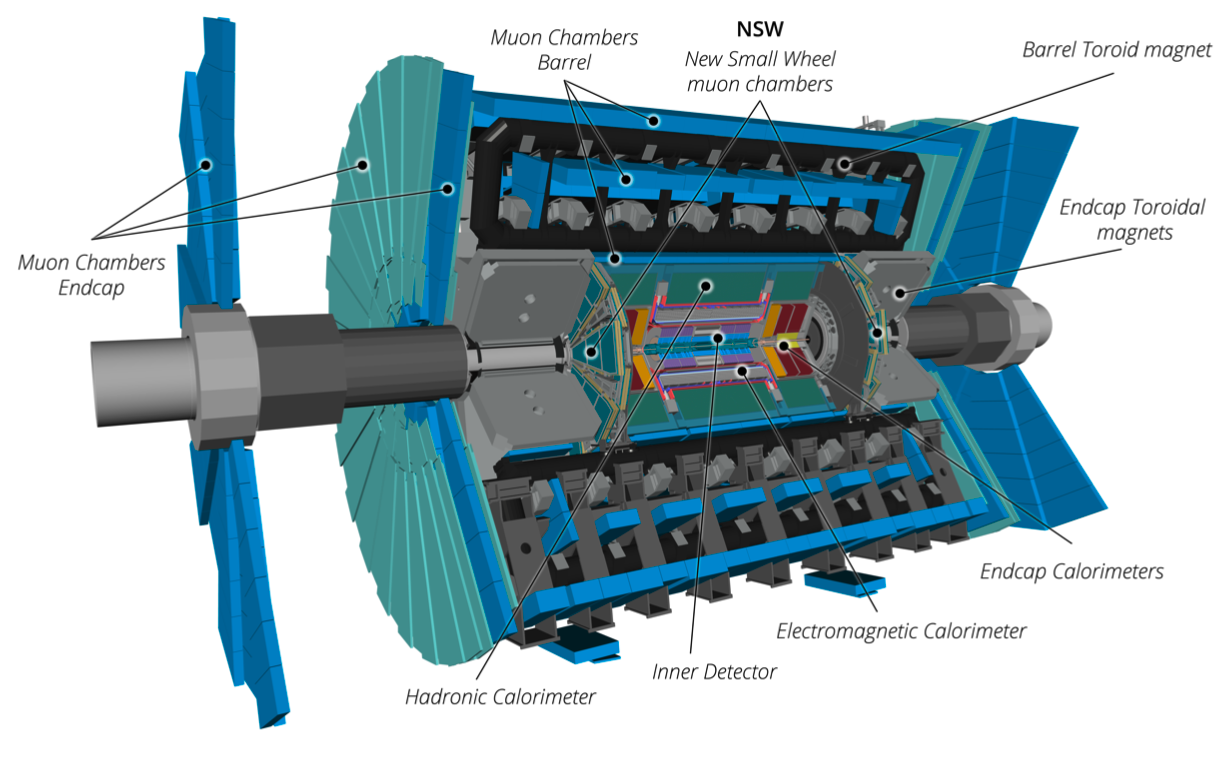
\includegraphics[width=.95\textwidth,keepaspectratio=true]{/Users/eparrish/Work/thesis/chapters/chapter3_experiment/images/ATLAS_3d_run3.png}
        % \vspace{1cm}
        \begin{figure}
        \begin{centering}
        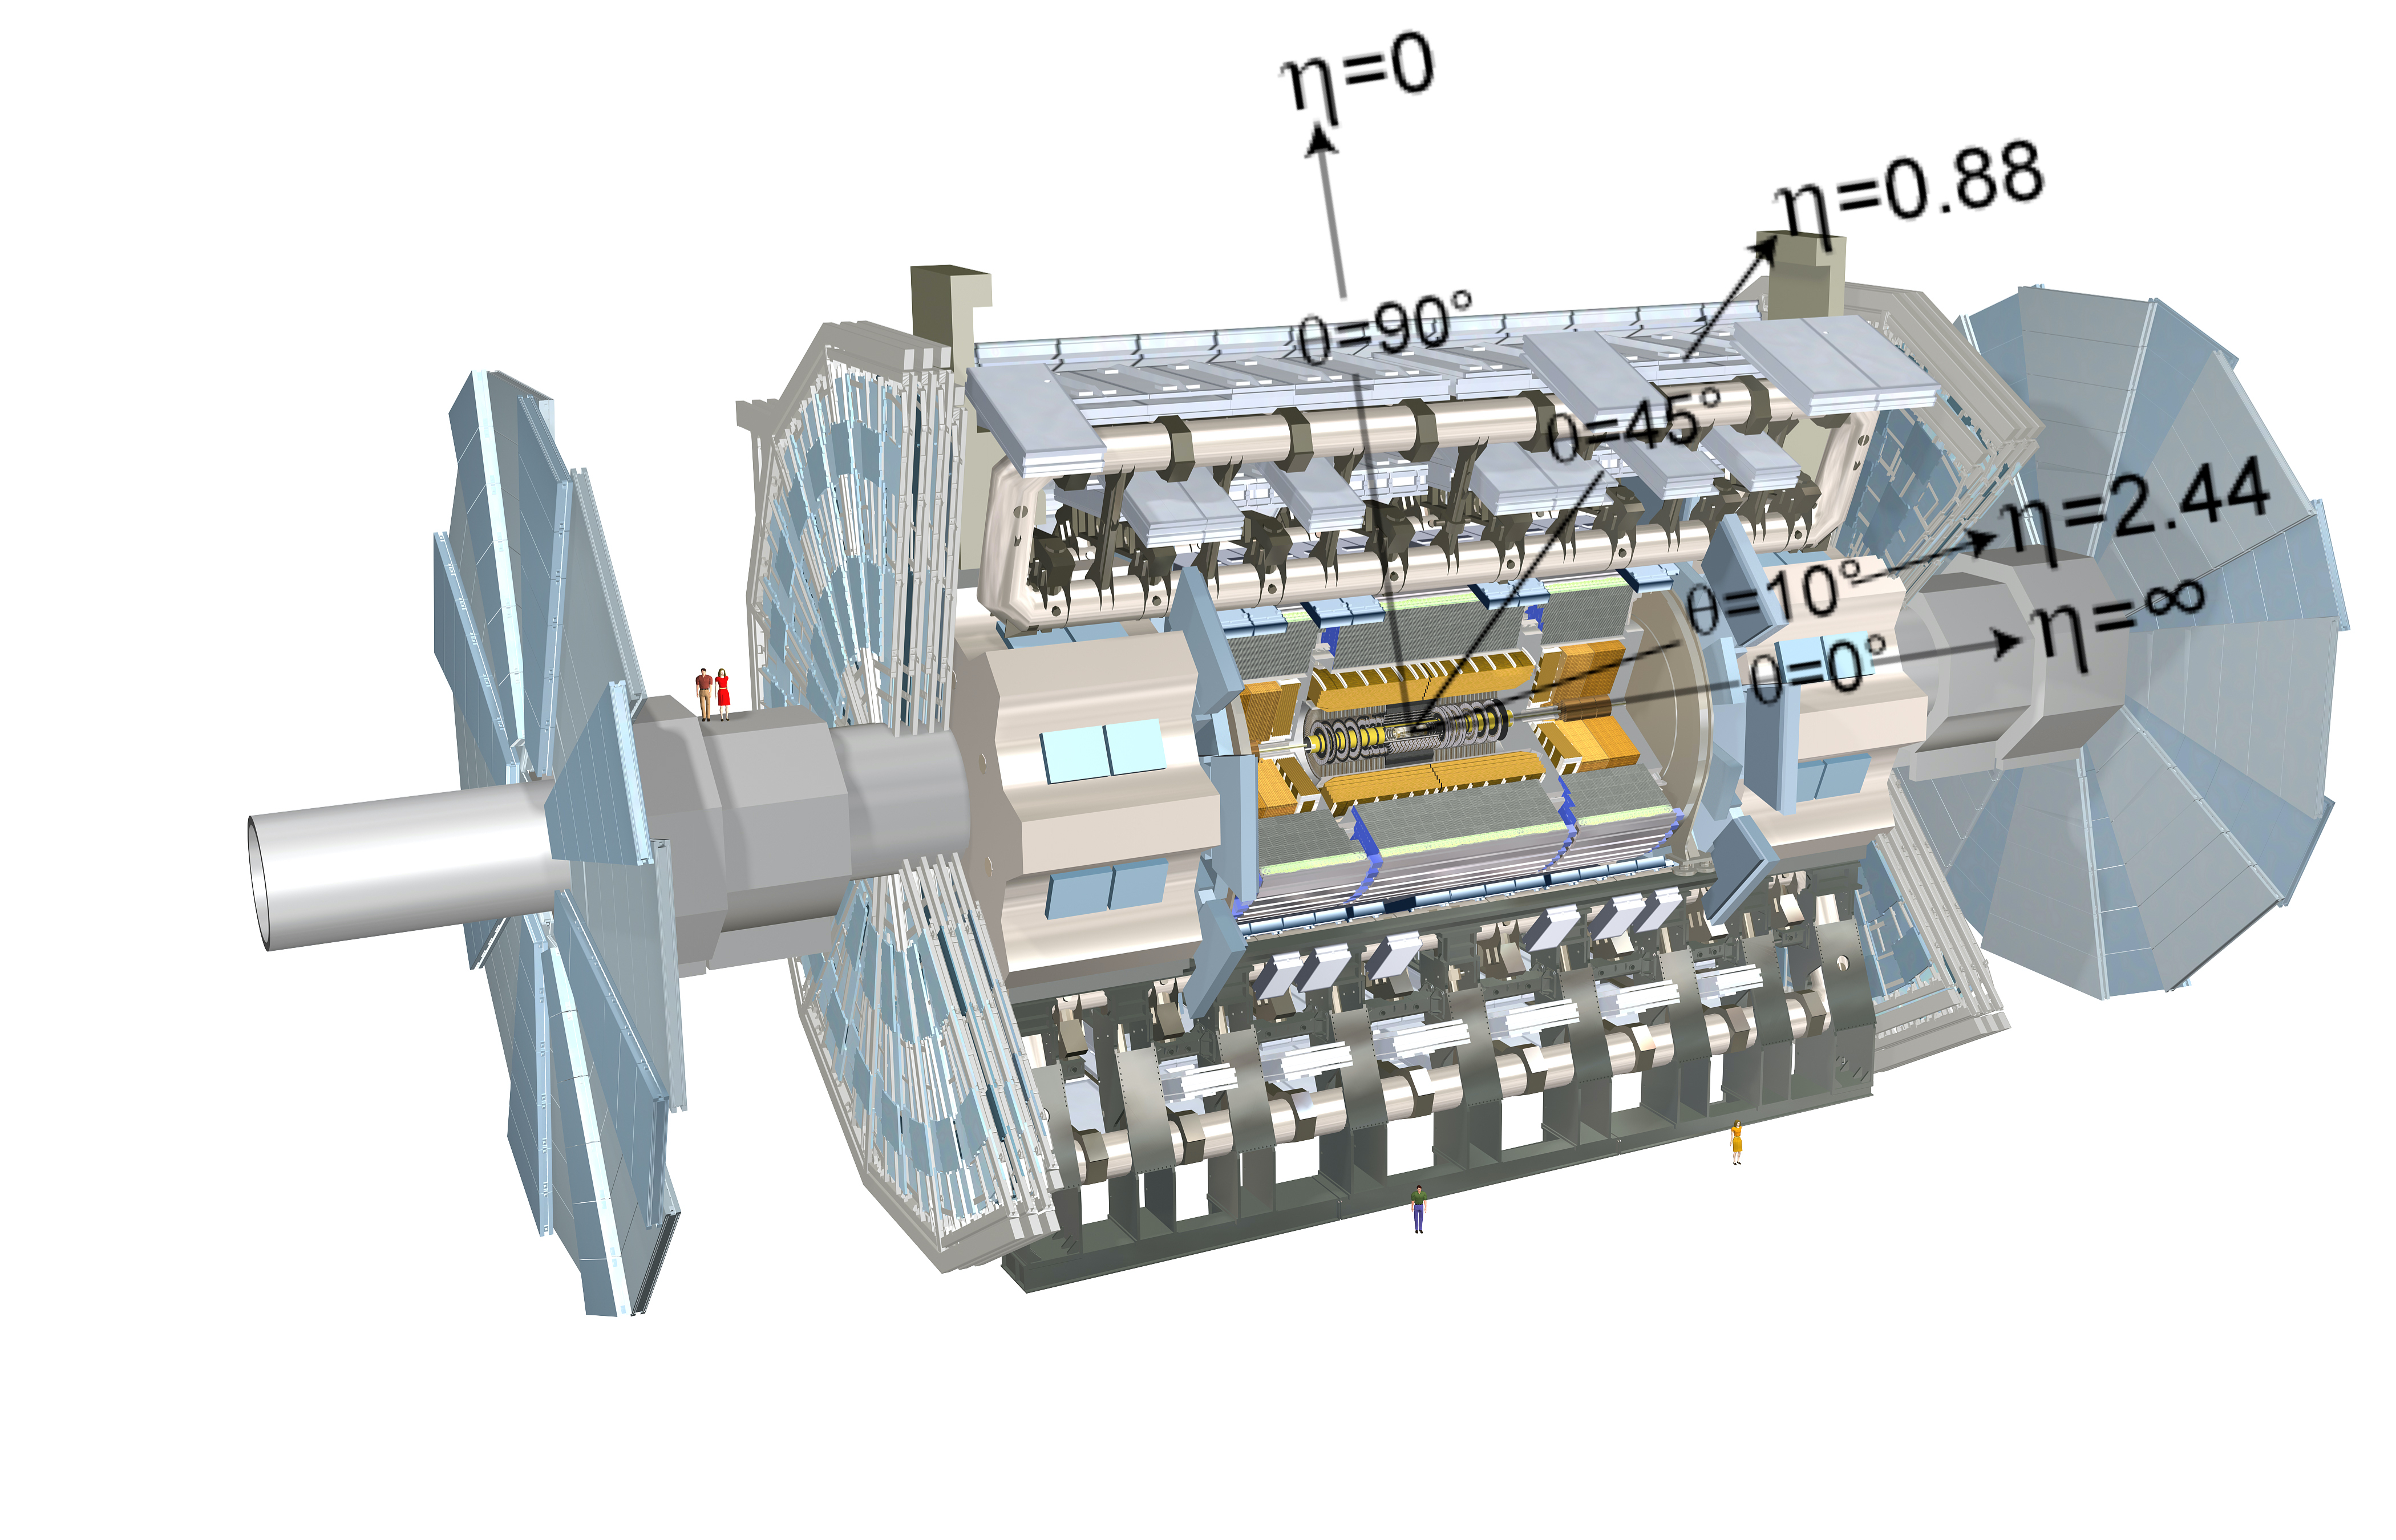
\includegraphics[width=\textwidth,keepaspectratio=true]{ATLAS_Full_Diagram.jpg}
        % \includegraphics[height=.35\textheight,keepaspectratio=true]{ATLASCrossSectionDiagram.png}
        \end{centering}
        \caption{\tiny \cite{atlas-schematics} \cite{pseudorapidity}}
        \end{figure}
      \end{columns}
    \end{frame}


    \begin{frame}[t]{Magnet System and Inner Detector}
     \begin{columns}[t]
      \column{.5\textwidth}
      \begin{itemize}
        \item Central solenoid
        \begin{itemize}
          \item 2 T magnetic field
          \item Bends charged particles in transverse plane
        \end{itemize}
        \item Toroid system
        \begin{itemize}
          \item 3.9 T magnetic field
          \item Bends charged particles ($\mu$) along beam axis
        \end{itemize}
      \end{itemize}

      % \begin{columns}
        % \column{.5\textwidth}
        % \centering
        % \includegraphics[height=.35\textheight,keepaspectratio=true]{/Users/eparrish/Work/thesis/chapters/chapter3_experiment/images/ATLASCrossSectionDiagram.png}
        % \column{.5\textwidth}
        \vspace{-.3cm}
        \begin{figure}
        \begin{columns}
        \column{.95\textwidth}
        \centering
        \includegraphics[height=.3\textheight,keepaspectratio=true]{/Users/eparrish/Work/thesis/chapters/chapter3_experiment/images/magnetSystems_3d.png}
        \column{.05\textwidth}
        \caption{\tiny \cite{atlas-schematics}}
        \end{columns}
        \end{figure}

      % \end{columns}

      \column{.5\textwidth}
        \begin{itemize}
          \item Inner detector (ID) 
          \begin{itemize}
              % \vspace{-.4cm}
              \item Tracks trajectories of charged particles
              \item Used to measure momentum in the transverse plane (\pt)
          \end{itemize}
        \end{itemize}
        \begin{columns}
        % \column{.5\textwidth}
        % \includegraphics[height=.25\textheight,keepaspectratio=true]{/Users/eparrish/Work/thesis/chapters/chapter3_experiment/images/ATLASCrossSectionDiagram.png}
        \column{.5\textwidth}
        % \begin{figure}
          % \begin{columns}
          %   \column{.95\textwidth}
          %     \centering
              \includegraphics[height=.25\textheight,keepaspectratio=true]{/Users/eparrish/Work/thesis/chapters/chapter3_experiment/images/ATLAS_ID_Highlight_Run2}
        %     \column{.05\textwidth}
        %       \caption{\tiny \cite{atlas-schematics}}
        %   \end{columns}
        % \end{figure}
        % \end{columns}
        \column{.5\textwidth}
        \centering

        % \begin{figure}
          \includegraphics[height=.3\textheight,keepaspectratio=true]{/Users/eparrish/Work/thesis/chapters/chapter3_experiment/images/ATLAS_ID_Run2}
          % \caption{\tiny \cite{atlas-schematics}}
        % \end{figure}
        \end{columns}
      \end{columns}
    \end{frame}

    \begin{frame}[t]{Calorimeters}
     \begin{columns}[t]
      \column{.45\textwidth}
        \begin{itemize}
          \item Important in jet, $\tau$, \Etm \, and $\mu$ identification and triggering
          \item Measure energy of charged particles
          \begin{itemize}
              \item Designed to fully absorb particles
              % \item Liquid argon`1g tile hadronic calorimeter
              % \begin{itemize}
              %   \item Forward hadronic calorimeters are liquid argon
              % \end{itemize}
          \end{itemize}
        \end{itemize}

      \centering
      \includegraphics[height=.35\textheight,keepaspectratio=true]{/Users/eparrish/Work/thesis/chapters/chapter3_experiment/images/ATLASCrossSectionDiagram.png}

      \column{.55\textwidth}
      % \hspace{2cm}
      \begin{figure}
        \begin{columns}
          \column{.95\textwidth}
            \centering
            \includegraphics[height=.2\textheight,keepaspectratio=true]{/Users/eparrish/Work/thesis/chapters/chapter3_experiment/images/ATLAS_Calorimeters_Highlight_Run2}
          \column{.05\textwidth}
            \caption{\tiny \cite{atlas-schematics}}
        \end{columns}
      \end{figure}
      \begin{figure}
        \includegraphics[height=.47\textheight,keepaspectratio=true]{/Users/eparrish/Work/thesis/chapters/chapter3_experiment/images/ATLAS_Calorimeters_Run2}
        \caption{\tiny \cite{atlas-schematics}}
      \end{figure}
      \end{columns}
    \end{frame}

    \begin{frame}[t]{Tile Calorimeter}
     \begin{columns}[t]
      \column{.55\textwidth}
        \begin{itemize}
          % \item Designed to measure hadron energy by fully absorbing particle showers
          \item Scintillating tile with steel absorber
          % \item Hadronic sampling calorimeter, covering $\abs{\eta} < 1.7$
          % \item Covers $\abs{\eta} < 1.7$
          % \item Important in jet, $\tau$, \Etm \, and $\mu$ identification and triggering
          \item I served as Data Quality Co-Coordinator for several years
          \begin{itemize}
            \item In Run-2 $99.65\%$ DQ efficiency \cite{DQ-Run2}
          \end{itemize}
        \end{itemize}

      \centering
      \vspace{-.2cm}
      \begin{columns}
      \column{.6\textwidth}
      \includegraphics[height=.4\textheight,keepaspectratio=true]{/Users/eparrish/Work/thesis/chapters/chapter3_experiment/images/ATLASCrossSectionDiagram.png}
      \column{.5\textwidth}
        \begin{figure}
          \begin{columns}
            \column{.95\textwidth}
            \centering
            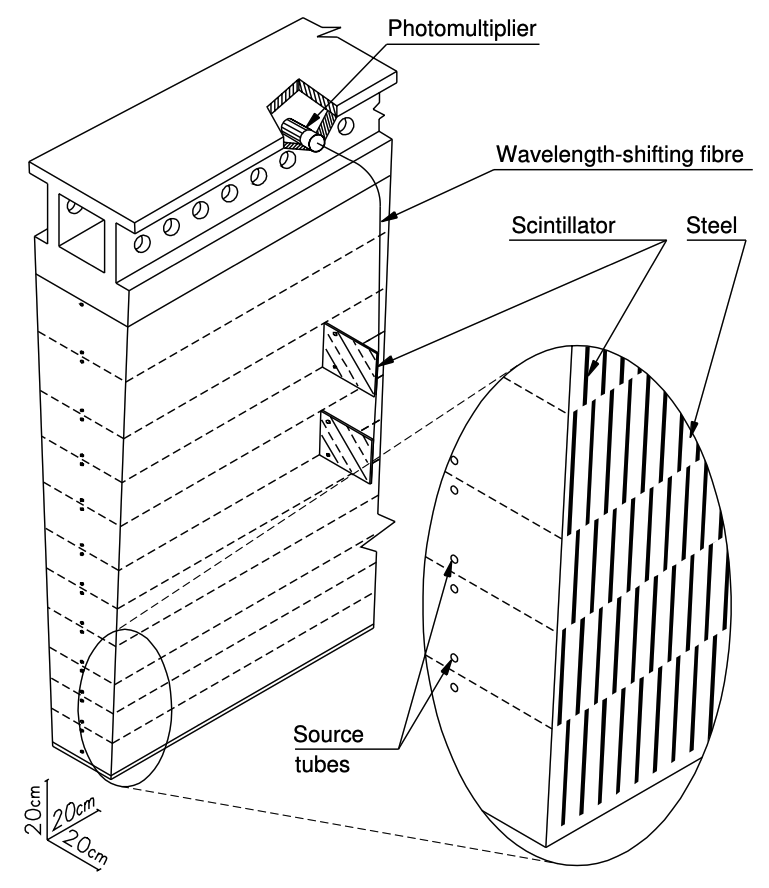
\includegraphics[height=.4\textheight,keepaspectratio=true]{/Users/eparrish/Work/thesis/chapters/chapter3_experiment/images/TileModuleCrossSection.png}
            \column{.05\textwidth}  
            \vspace{1cm}
            \caption{\tiny \cite{ATLAS-tile}}
          \end{columns}
        \end{figure}
      \end{columns}


      \column{.4\textwidth}
        \centering
        \begin{columns}
        \centering
        \column{.5\textwidth}
        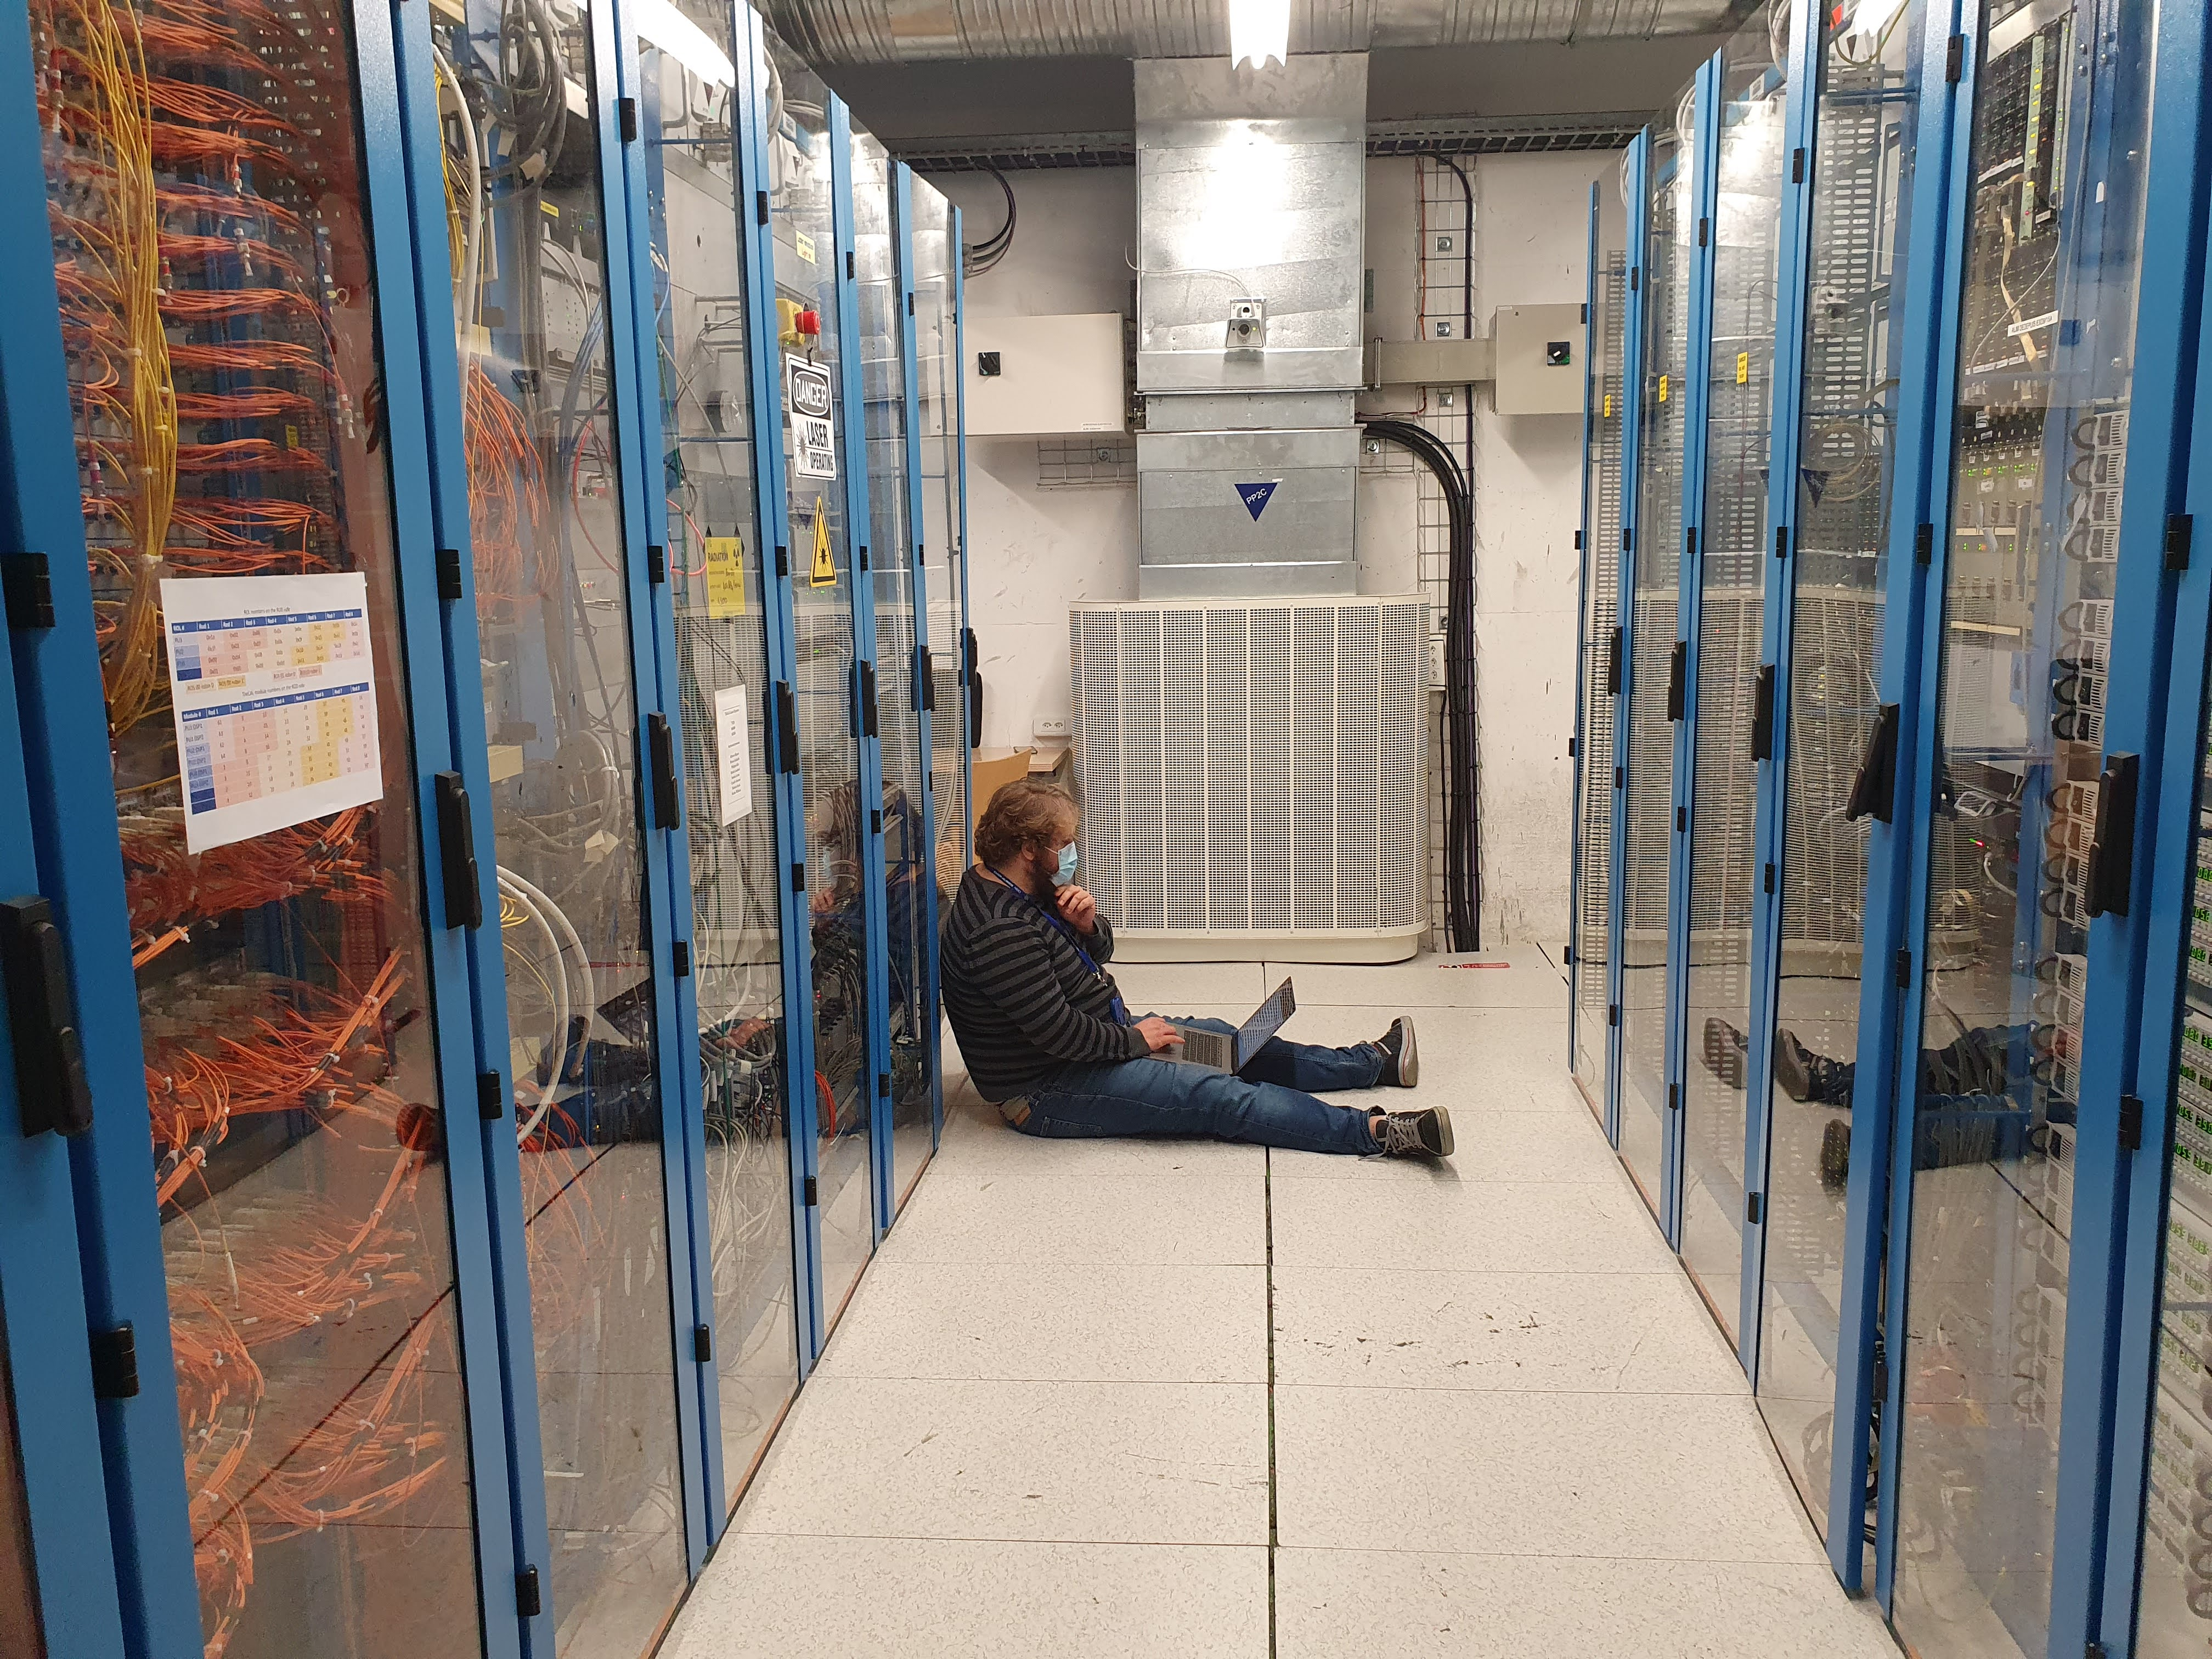
\includegraphics[height=.33\textheight,keepaspectratio=true]{Hard_At_Work.jpg}
        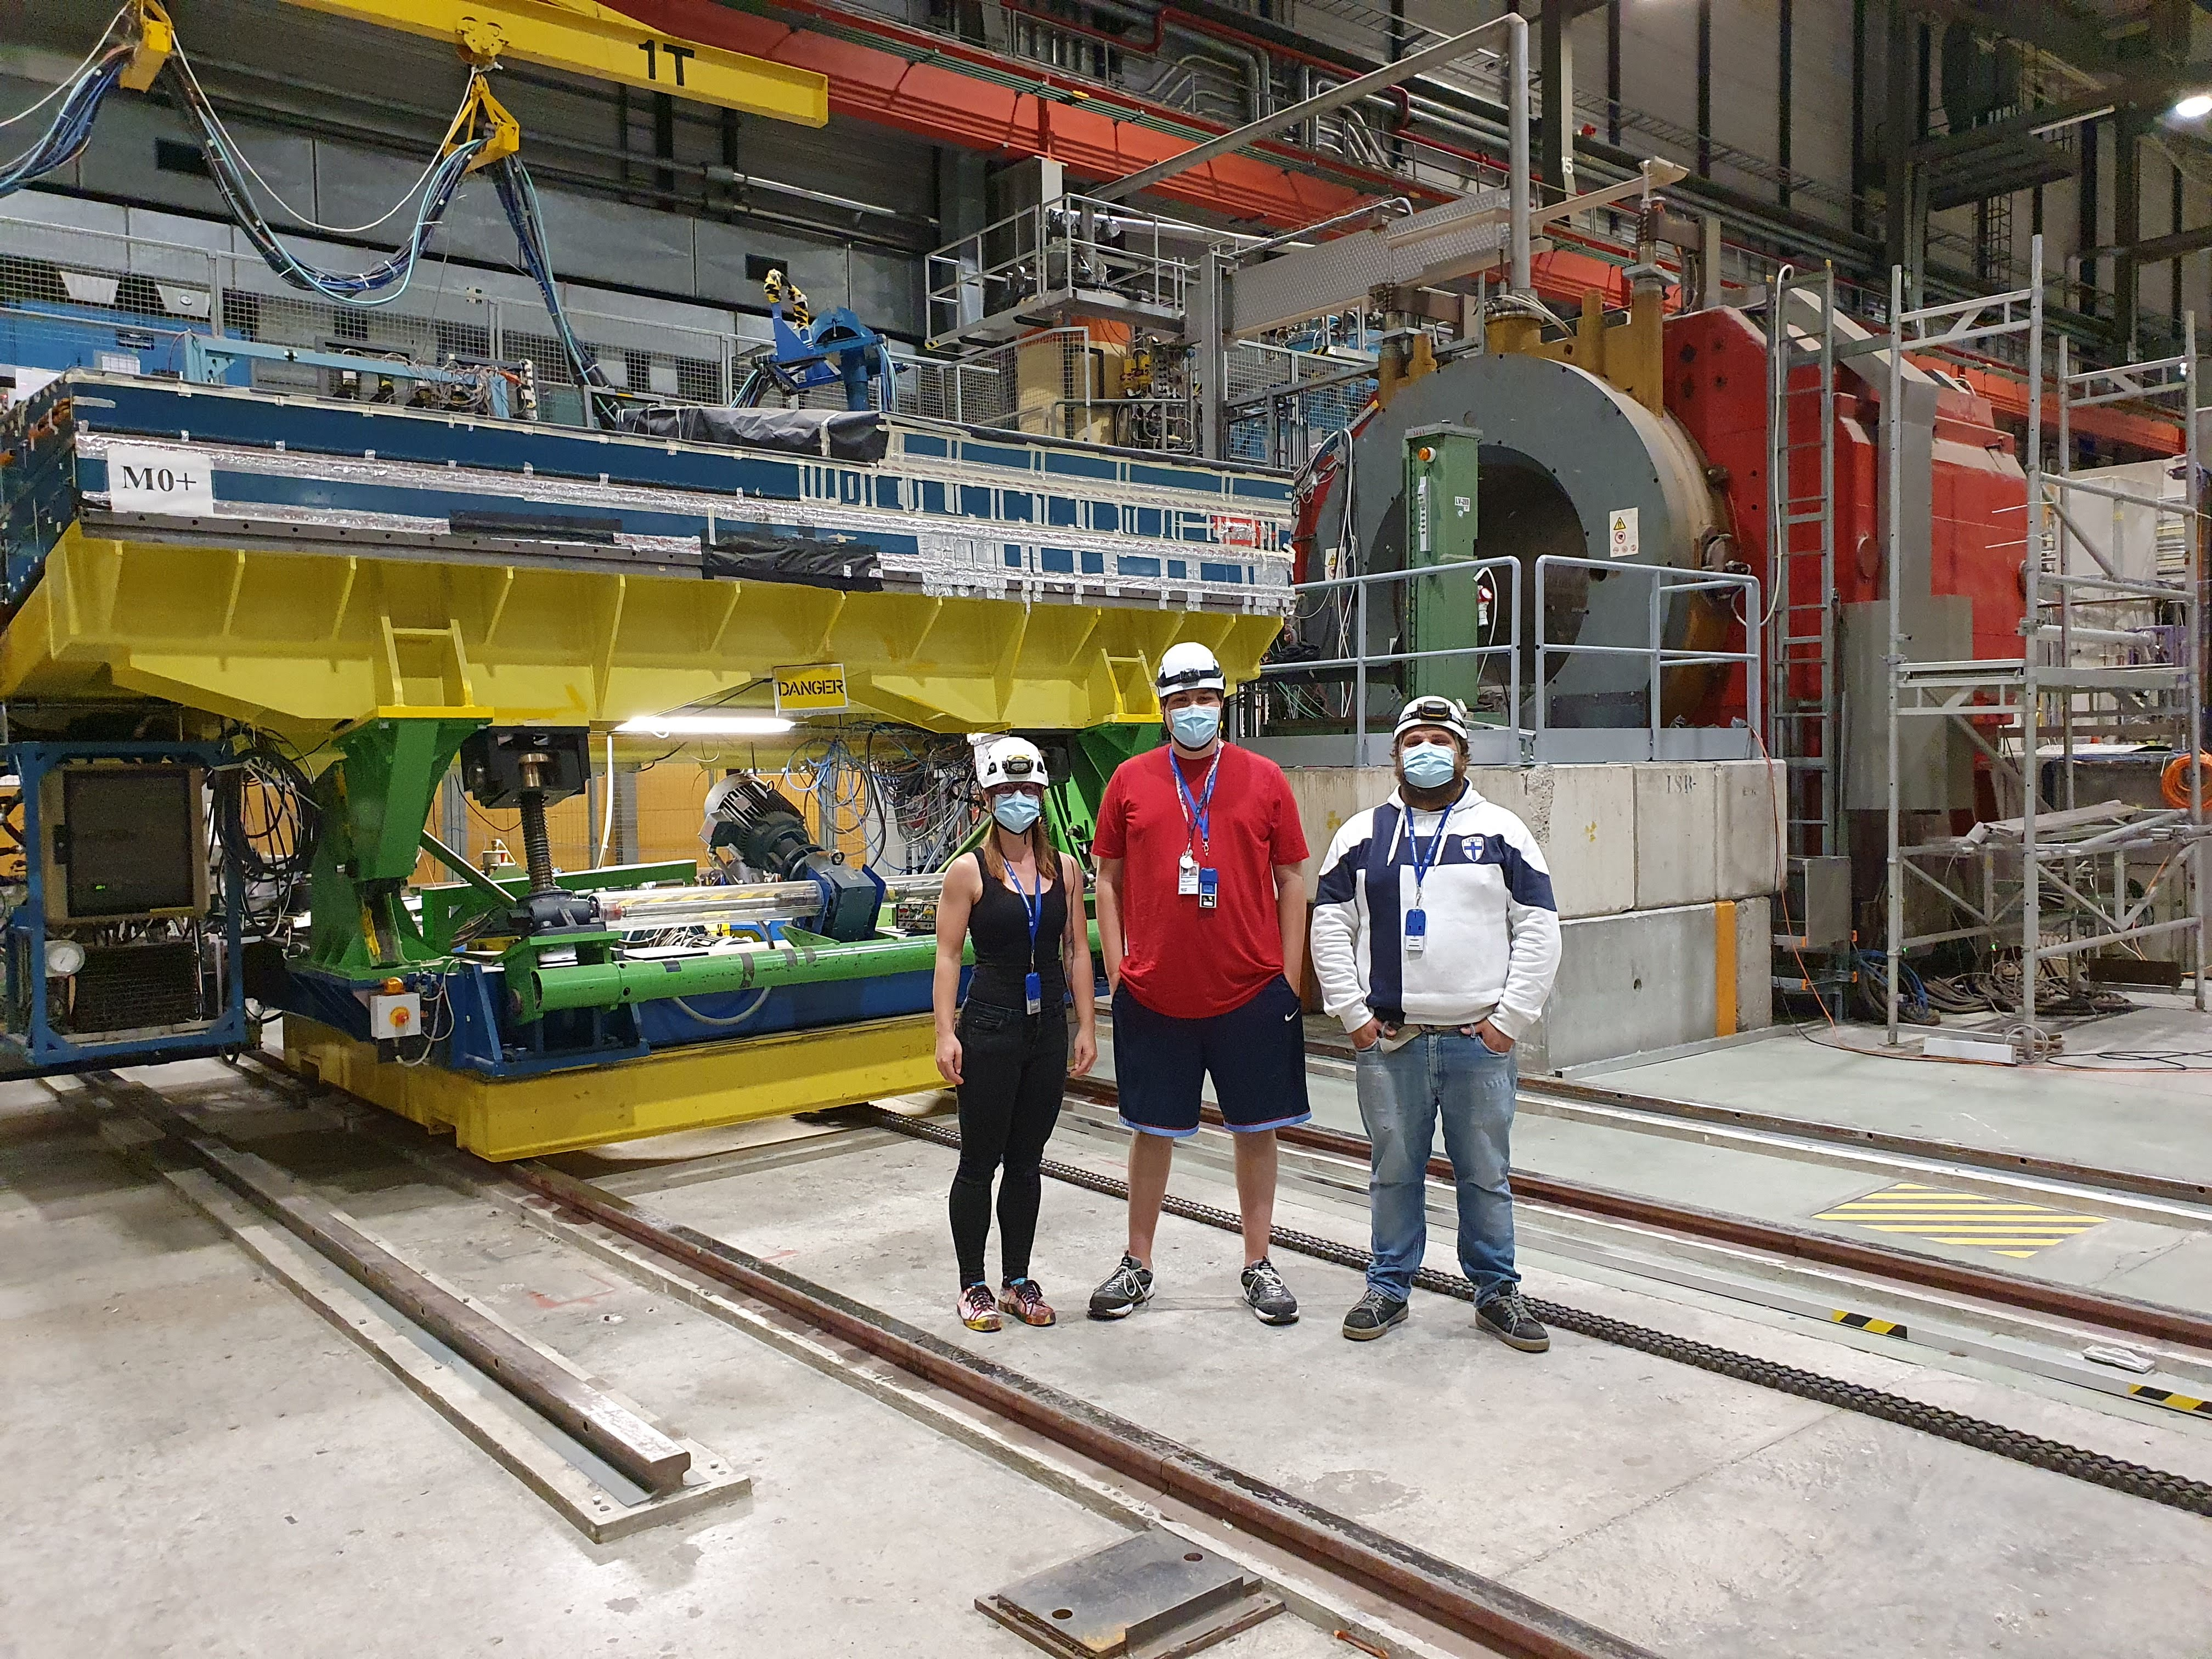
\includegraphics[height=.33\textheight,keepaspectratio=true]{TileTestBeamSetup_Michaela_Will_Me.jpg}
        \column{.5\textwidth}
        \centering
        % 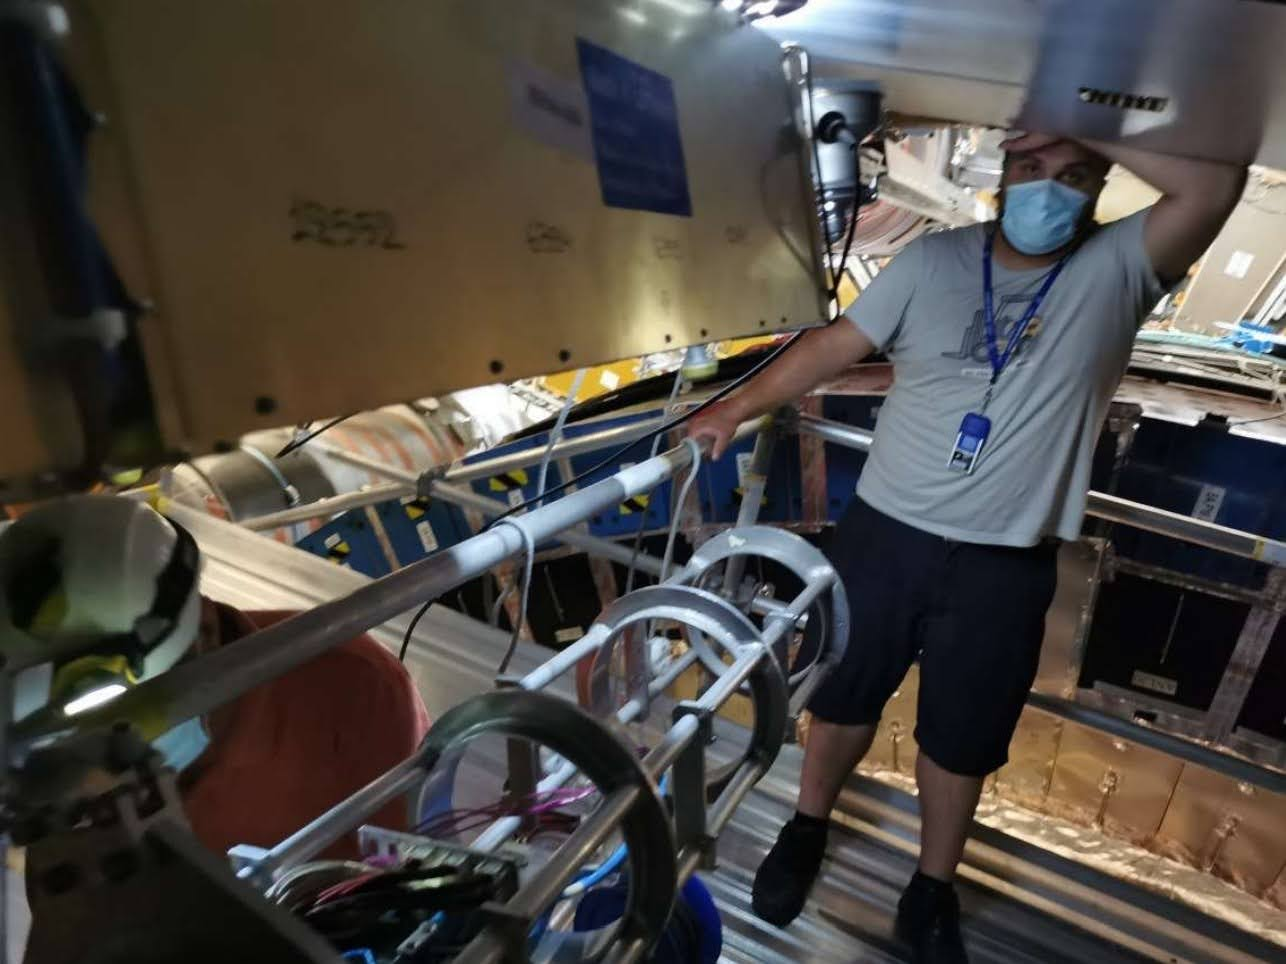
\includegraphics[height=.33\textheight,keepaspectratio=true]{OnLBA14.jpg}
        % 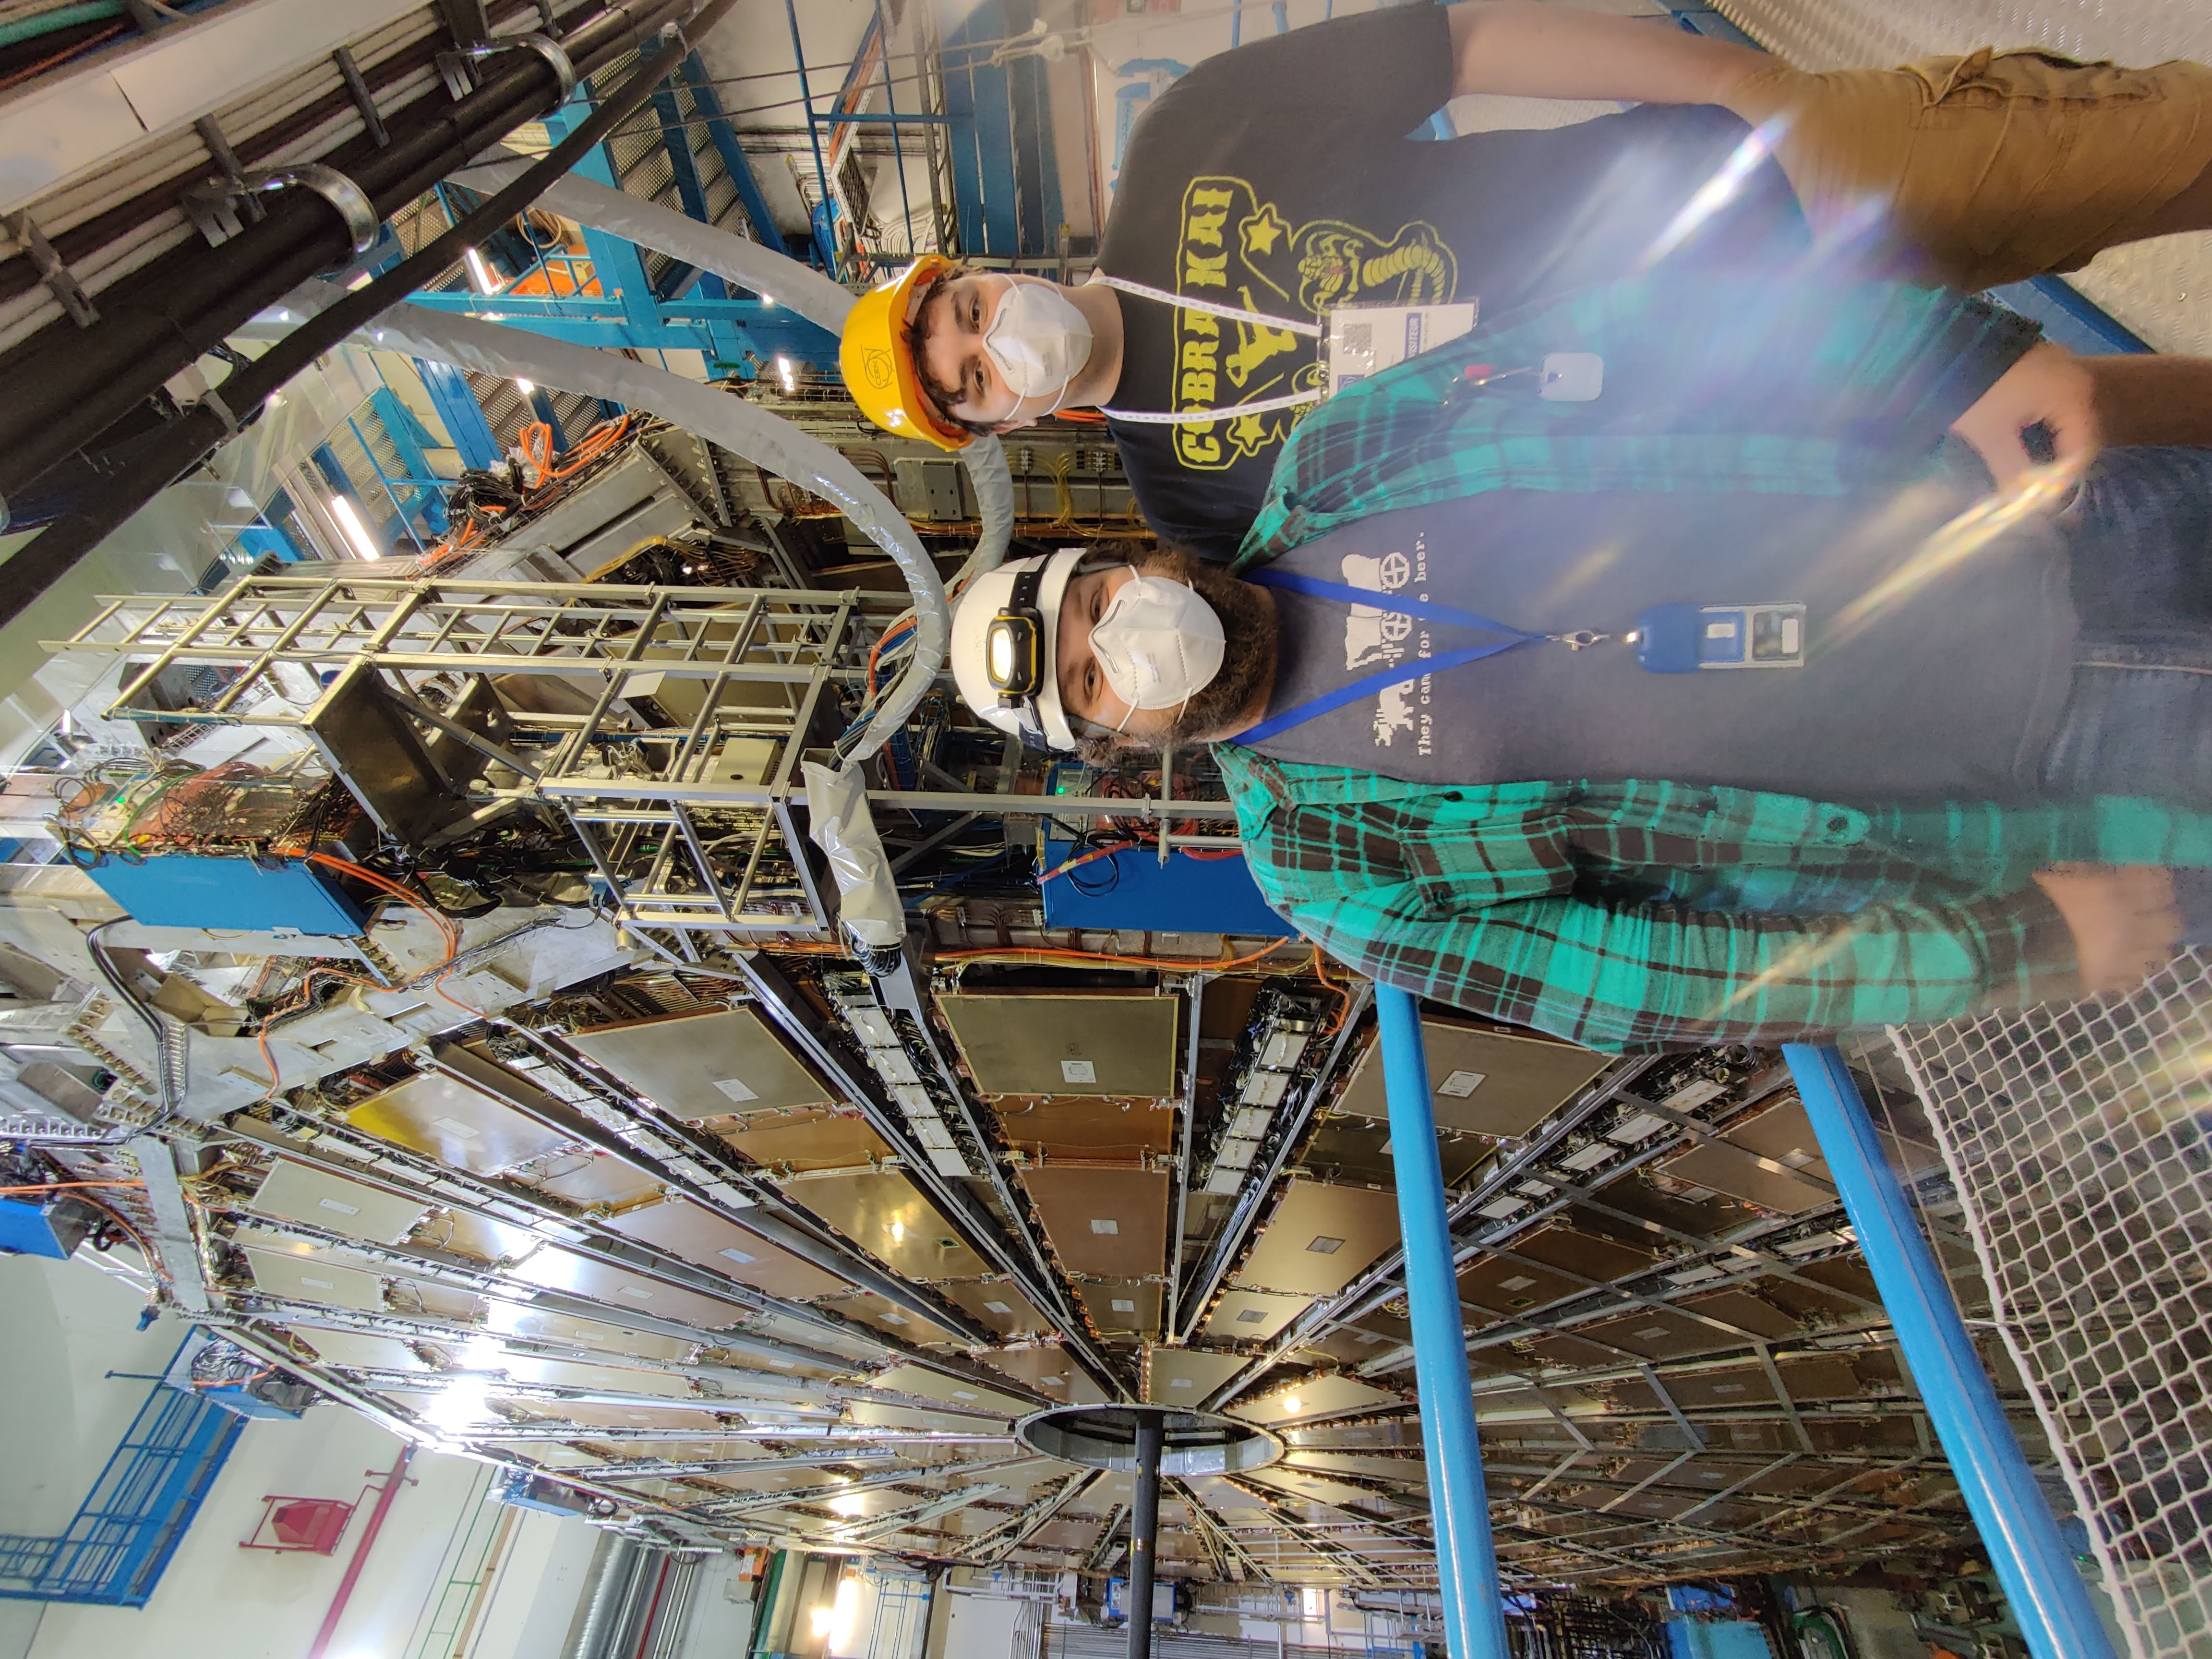
\includegraphics[height=.33\textheight,keepaspectratio=true,angle=-90,origin=c]{WillAndMeAtATLAS.jpg}
        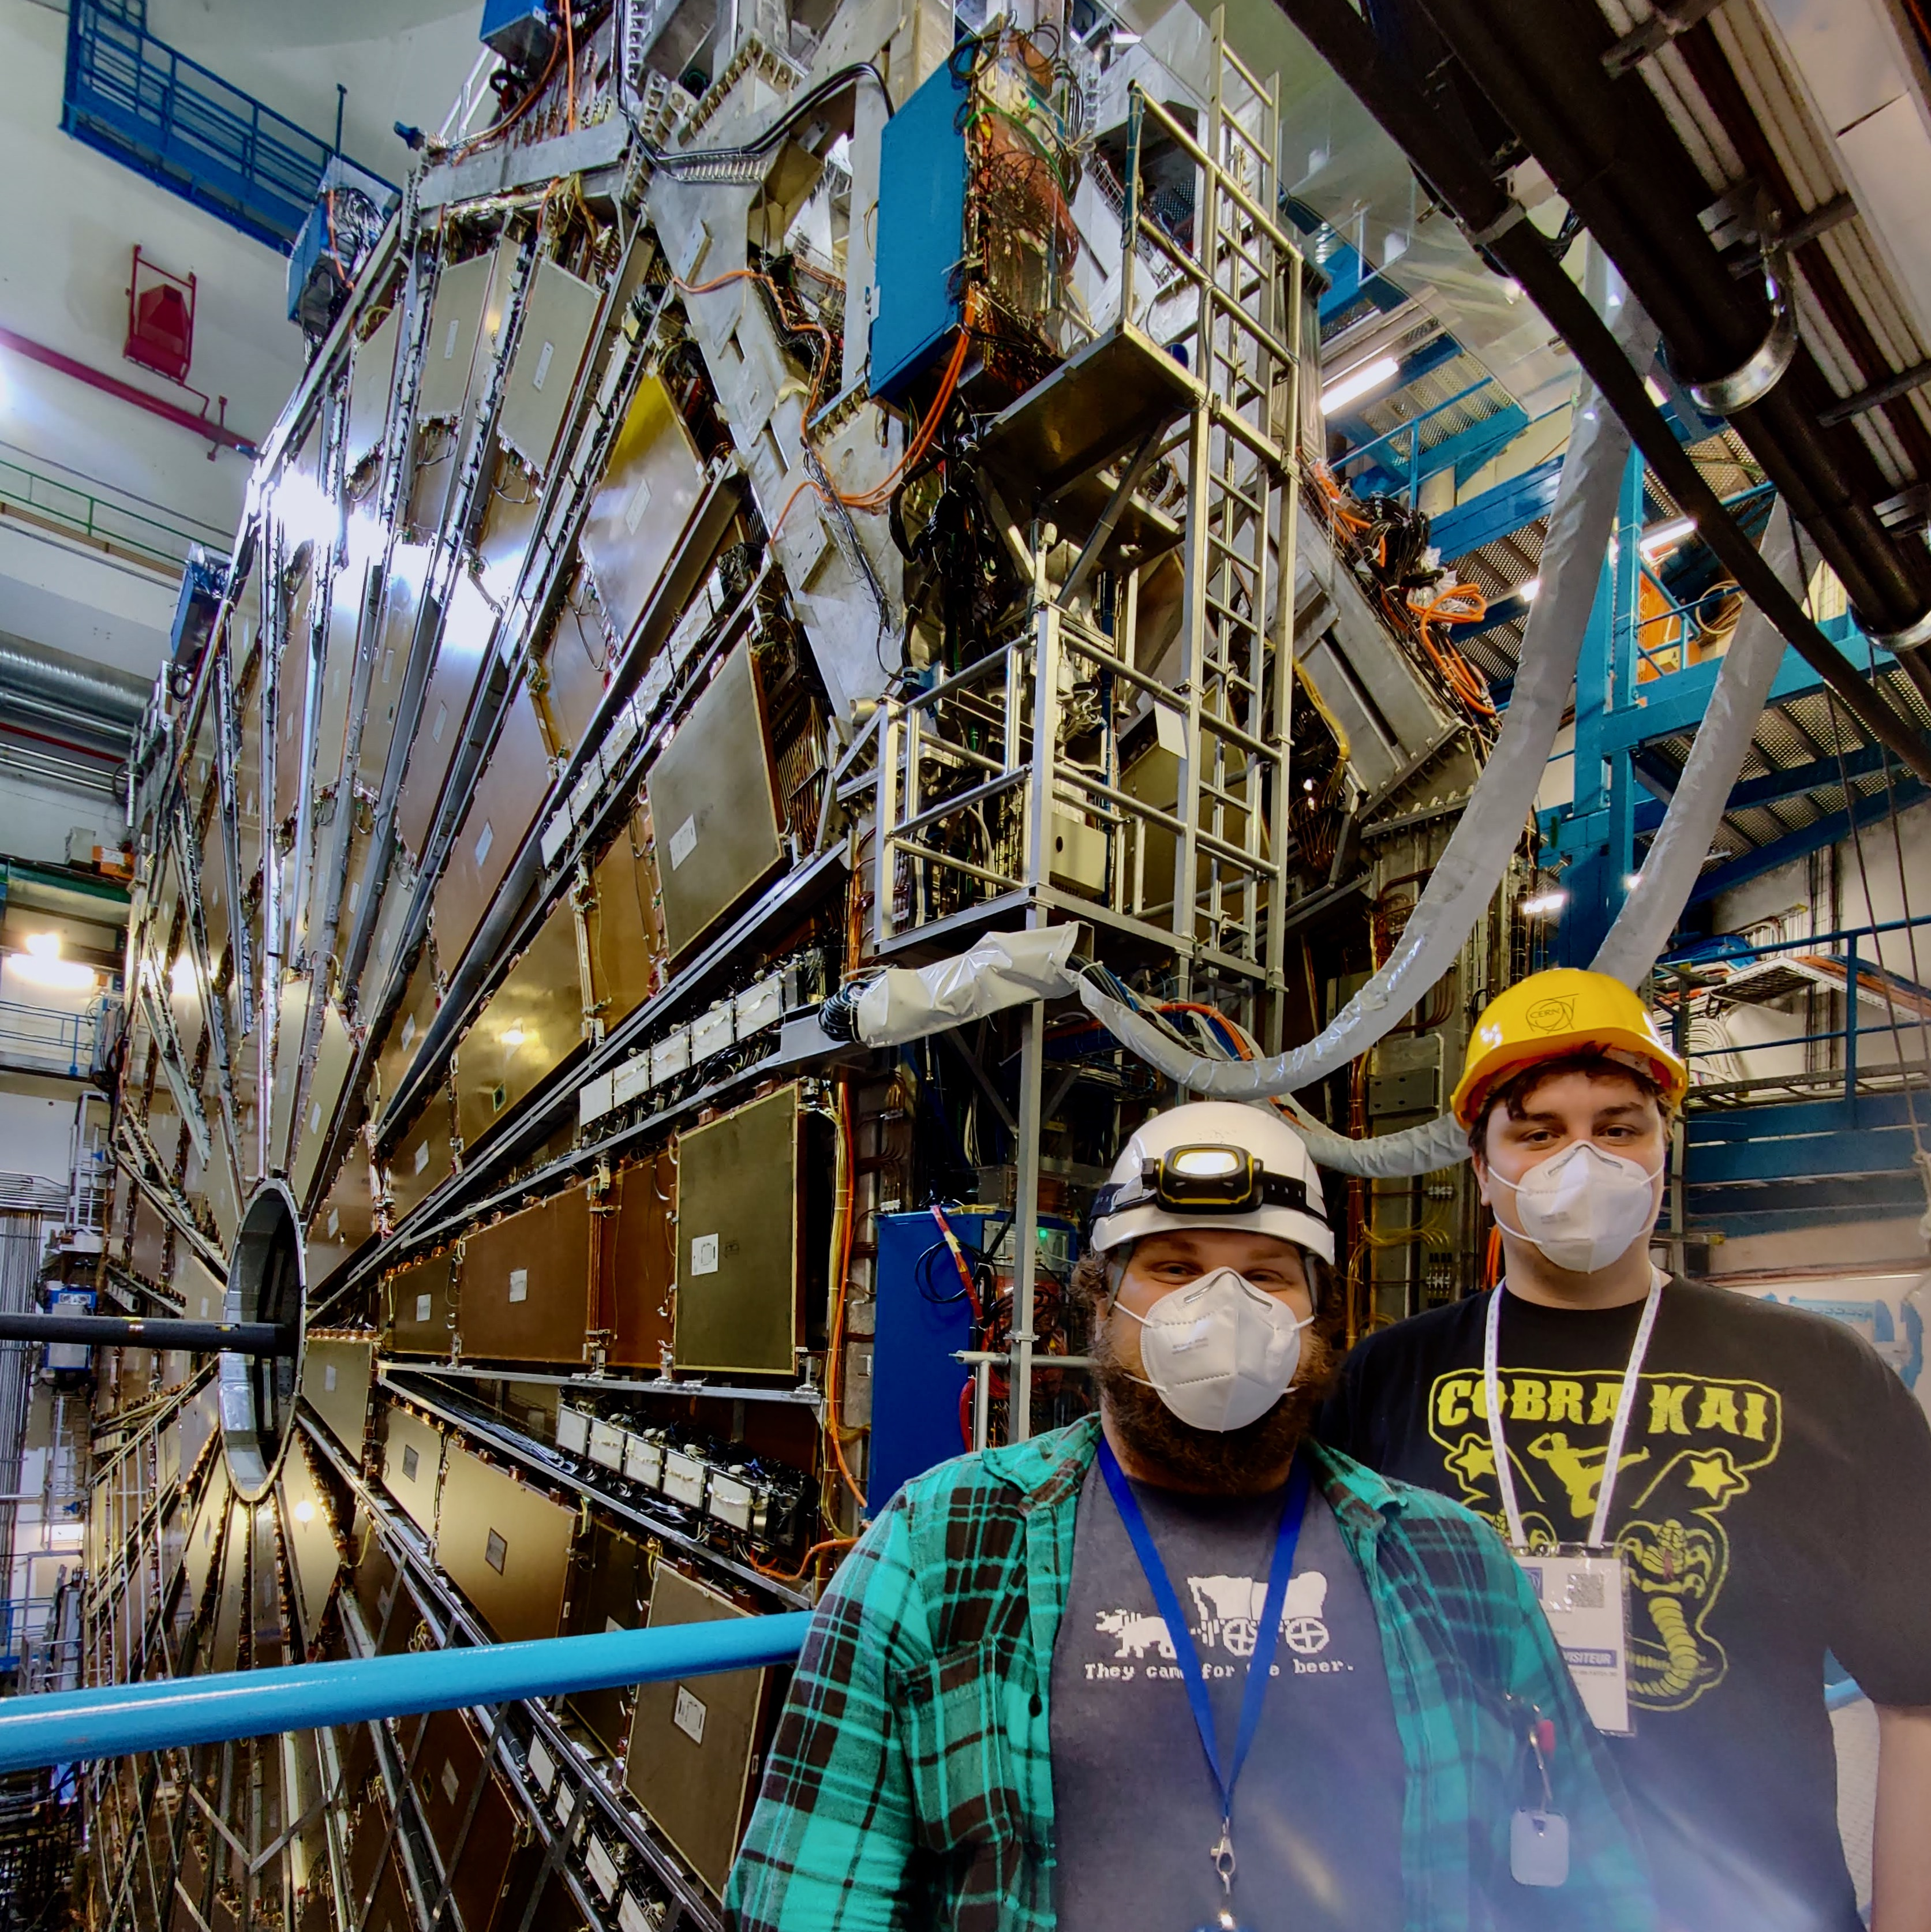
\includegraphics[height=.33\textheight,keepaspectratio=true]{WillAndMeAtATLAS.jpeg}
        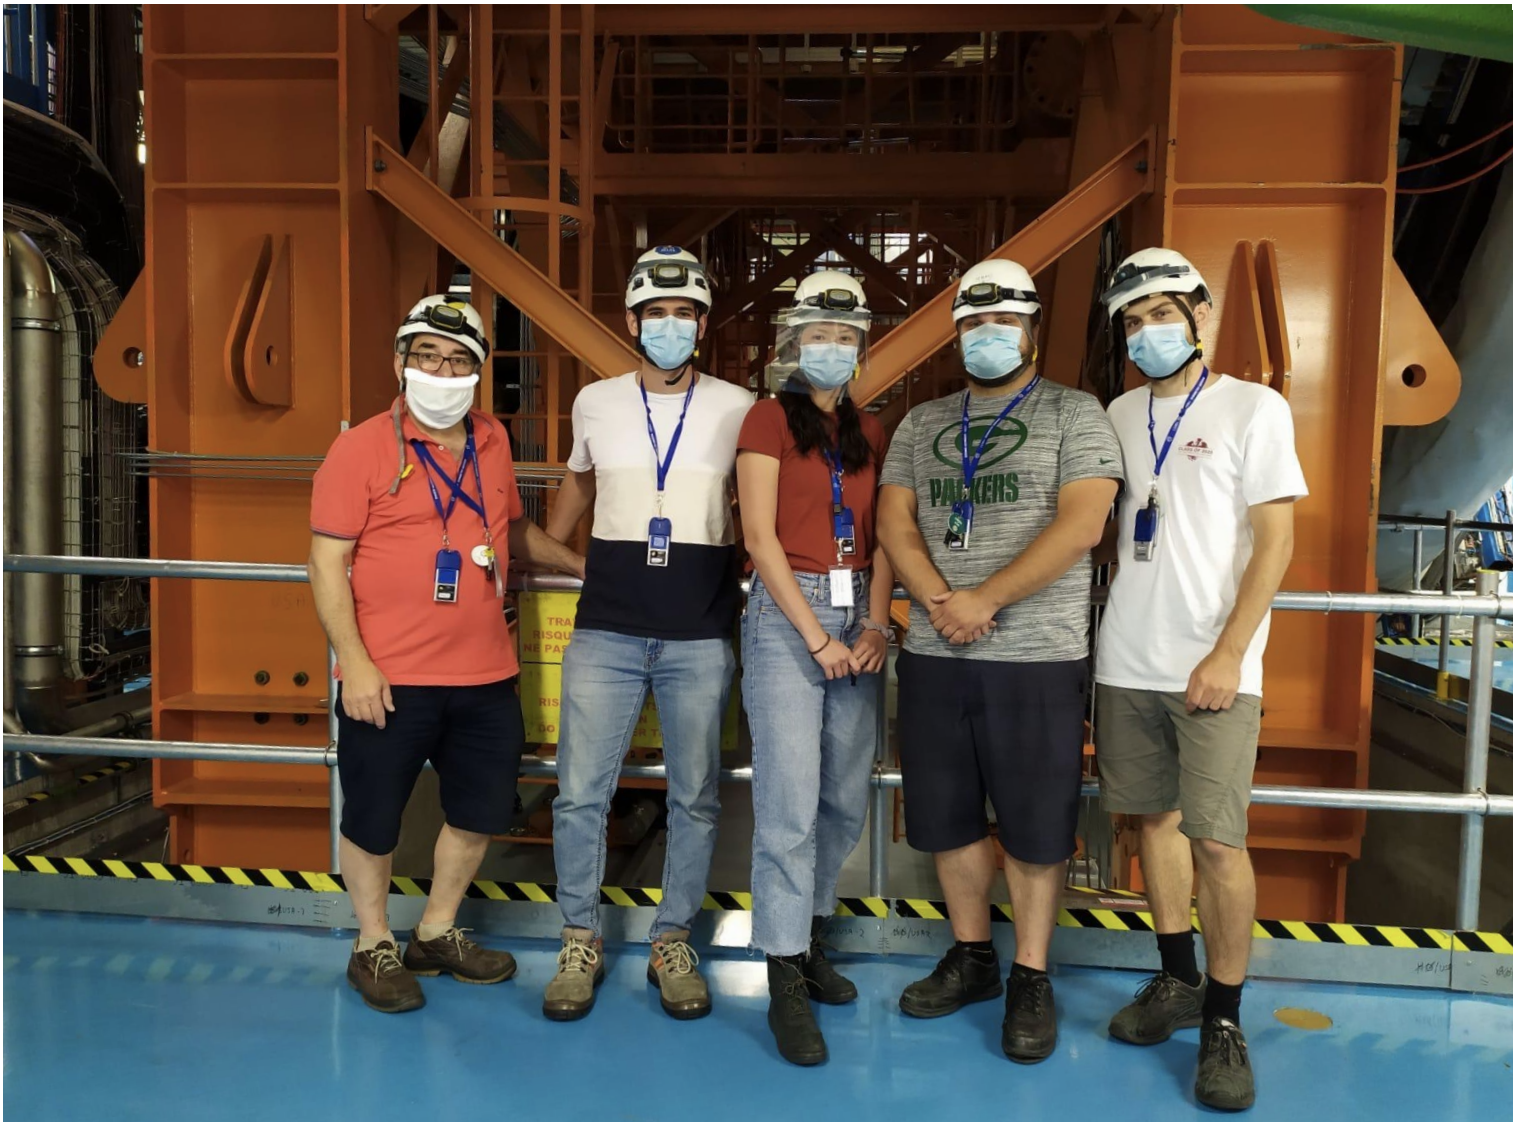
\includegraphics[height=.33\textheight,keepaspectratio=true]{TileMaintenanceTeamJune2020.png}

        \end{columns}
      \end{columns}
    \end{frame}

    \begin{frame}[t]{Muon System and Trigger}
     \begin{columns}[t]
      \column{.45\textwidth}
        \begin{itemize}
          \item Muon Spectrometers (MS) detect and measure $\mu$
          \begin{itemize}
            \item Muons are minimally ionizing
            \item $\mu$ reach the outermost region of the detector
            \item Information combined with inner detector to reconstruct $\mu$
          \end{itemize}
          % \item Muon spectrometers track trajectory
        \end{itemize}

      \vspace{-.4cm}
      \begin{columns}
        \column{.5\textwidth}
        \centering
        \includegraphics[height=.3\textheight,keepaspectratio=true]{/Users/eparrish/Work/thesis/chapters/chapter3_experiment/images/ATLASCrossSectionDiagram.png}
        \column{.5\textwidth}
        \centering
        \begin{figure}
          \includegraphics[height=.3\textheight,keepaspectratio=true]{/Users/eparrish/Work/thesis/chapters/chapter3_experiment/images/ATLAS_Muon_System_Run2.png}
          \caption{\tiny \cite{atlas-schematics}}
        \end{figure}
      \end{columns}

      \column{.55\textwidth}
      \centering
      \begin{itemize}
        \item Trigger System
        \begin{itemize}
          \item Need to quickly sort through data and decide if a collision is interesting or not
          \item Mix of hardware and software
        \end{itemize}
      \end{itemize}
        \begin{figure}
          \centering
          \includegraphics[height=.4\textheight,keepaspectratio=true]{/Users/eparrish/Work/thesis/chapters/chapter3_experiment/images/tdaq-run2-schematic2017.png}
          \caption{\tiny \cite{TDAQ_Diagram}}
        \end{figure}

      \end{columns}
    \end{frame}

  \subsection{Object Reconstruction}

    \begin{frame}[t]{Reconstruction: \Etm and \bjets}
     \begin{columns}[t]
      \column{.5\textwidth}
        \begin{itemize}
          \item Particles like $\nu$ do not leave a signature within ATLAS
          \item Instead, infer their presence through momentum conservation
          \begin{itemize}
            \item Negative vector sum of all objects in a collision event
          \end{itemize}
        \end{itemize}
        \centering
        \includegraphics[width=.5\textwidth,keepaspectratio=true]{MET_Diagram.png}

      \column{.5\textwidth}
      \begin{itemize}
        \item b quark initiated hadronic showers are identified by a displaced vertex, etc.
        \item Reconstructed as a jet, tagged as a \bjet
        \begin{itemize}
          \item Algorithms designed to identify \bjets called taggers \cite{b-tagging}
        \end{itemize}
      \end{itemize}
      \begin{figure}[!ht]
      \centering
      \includegraphics[width=.7\textwidth,keepaspectratio=true]{chapters/chapter5_eventreconnstruction/images/b-jet-schetch.png}
      \caption{\tiny \cite{bjet-trigger}}
      \end{figure}
      \end{columns}
    \end{frame}

    \begin{frame}[t]{Reconstruction: $e$ and $\mu$}
      \begin{columns}[t]
        \column{.5\textwidth}
        \begin{itemize}
          \item Electron identification
          \begin{itemize}
            \item Information from the ID and showers in the EM calorimeter are combined
            \item This analysis uses tight ID and tight isolation requirements
          \end{itemize}
        \end{itemize}

        \column{.5\textwidth}
        \begin{itemize}
          \item $\mu$ identification
          \begin{itemize}
            \item Information from the ID is combined with the MS
            \item This analysis uses tight ID and tight isolation requirements
          \end{itemize}
        \end{itemize}
      \end{columns}
      \centering
      \includegraphics[height=.45\textheight,keepaspectratio=true]{/Users/eparrish/Work/thesis/chapters/chapter3_experiment/images/ATLASCrossSectionDiagram.png}
      
    \end{frame}

    \begin{frame}[t]{Reconstruction: $\tau$ leptons}
      \begin{columns}
        \column{.5\textwidth}
        \begin{itemize}
          \item $\tau$ leptons typically decay before they interact with the detector
          % \item $\tau$ lepton decays are messy and difficult to reconstruct
          \item $\tau$ leptons decay hadronically $\approx 65\%$ of the time
          \begin{itemize}
            \item leptonic decays are not considered
          \end{itemize}
          \item Number of charged hadrons $(\pi^{\pm})$ in decays defines number of prongs
          \begin{itemize}
            \item 1 $\pi^{\pm}$ occurs 72\% of the time
            \item 3 $\pi^{\pm}$ occurs 22\% of the time
            \item Of these decays, 68\% contain $> 1\, \pi^{0}$
          \end{itemize}
          \item $\nu_{\tau}$ are also produced in these decays
          \begin{itemize}
            \item  Only visible part of $\tau$ can be reconstructed
          \end{itemize}
        \end{itemize}

        \column{.5\textwidth}
        \centering
        \begin{figure}
        \includegraphics[width=.45\textwidth,keepaspectratio=true]{tau_hadronic_decay.png}
        % \caption{\tiny }
        \end{figure}
        \begin{figure}
        \includegraphics[width=.45\textwidth,keepaspectratio=true]{jet_particle.png}
        \caption{\tiny \cite{tau-diagrams}}
        \end{figure}
        \begin{itemize}
          \item Reconstruction is imperfect
          \begin{itemize}
            \item Misidentification of particles is a large source of background
          \end{itemize}
        \end{itemize}
      \end{columns}
    \end{frame}

\section{Simulation }
  
  \begin{frame}[t]{Simulation}
     \begin{columns}[t]
      \column{.5\textwidth}
        \begin{itemize}
          \item Incredibly detailed simulations are used to create analysis strategy
            \begin{itemize}
              \item Entire data flow from collision to detector readout is simulated
              %   \item Thoroughly verified by many experiments and dedicated test beams
              \item Many different options to generate simulations
              \begin{itemize}
                \item Some excel at specific tasks and not great at others
              \end{itemize}
            \end{itemize}
          \item Control regions are used to verify simulation agreement with data
        \end{itemize}
        % \centering
        % \includegraphics[width=.45\textwidth,keepaspectratio=true]{/Users/eparrish/Work/thesis/chapters/chapter4_simulation/images/tth_hadronization_gen.png}

      \column{.5\textwidth}
        \begin{figure}
        \centering
        \includegraphics[width=\textwidth,keepaspectratio=true]{/Users/eparrish/Work/thesis/chapters/chapter4_simulation/images/Simulation_Chain.png}
        \caption{\tiny \cite{Wanotayaroj:2242196}}
        \end{figure}
      \end{columns}
  \end{frame}

% \section{Event Reconstruction }
  
%   \begin{frame}[t]{Particle Identification}
%      \begin{columns}
%       \column{.75\textwidth}
%         \begin{itemize}
%           \item
%         \end{itemize}

%       \column{.25\textwidth}

%       \end{columns}
%   \end{frame}

\section{\HpmLong }
  
  \begin{frame}[t]{Analysis Overview}
      \begin{columns}[t]

        \column{.75\textwidth}
            \vspace{-20mm}
            \begin{itemize}
              \item Search for singly charged \Hpm decaying to \taunu over a wide mass range
                \begin{itemize}
                  \item Low mass $ (\mHpm < m_{t})$:
                  % \begin{itemize}
                  %   \item $90 \leq m_{H^{\pm}} \leq 130$ GeV
                  % \end{itemize}
                  \item Intermediate mass*  $(\mHpm \simeq m_{t})$
                  % \begin{itemize}
                  %   \item $140 \leq m_{H^{\pm}} \leq 190$ GeV
                  % \end{itemize}
                  \item High mass $(\mHpm > m_{t})$
                  % \begin{itemize}
                  %   \item $200 \leq m_{H^{\pm}} \leq 2000$ GeV
                  % \end{itemize}
                \end{itemize}
              % \item Associated $\tau$ is required to decay hadronically
              \item Dominant backgrounds
              \vspace{-3mm}
            \begin{table}
              \tiny
              \resizebox{\linewidth}{!}{
              \rowcolors{1}{}{NIUgray}
              \begin{tabular}{l | l}
              \textbf{Backgrounds w/ prompt hadronic $\tau$} & \textbf{Backgrounds w/ fake $\tau$} \\
              \hline \hline
              $t\bar{t}$ estimated with simulation       & Fake $j \rightarrow \tau$ estimated with data driven fake factor method \\
              $V+jets$ estimated with simulation         & Fake $\ell \rightarrow \tau$ estimated with simulation, validated on $Z \rightarrow ee$\\
              VV estimated with simulation & \\
              \end{tabular}}
            \end{table}
            \item Classifier score is used as the final discriminant 
            % \item This talk will cover $36.1 \mathrm{fb}^{-1}$ and the current edition of this analysis
            \end{itemize}

            \vspace{-.45cm}
            \begin{table}
              \footnotesize
              \resizebox{\linewidth}{!}{
              \rowcolors{1}{}{NIUgray}
              \begin{tabular}{l | l | l | l | l | l | l | l | l | l | l | l} 
                \textbf{Sub-Channel} \\ \hline \hline
                {\large\textbf{$\tau + jets$ SR }} & $E^{miss}_{T}$ Trigger & \specialcell{1 hadronic $\tau$ \\ $p_{T}^{\tau} > 40$ GeV} & \specialcell{0 $\ell$ (e or $\mu$) \\ $p_{T}^{\ell} > 20$ GeV} & \specialcell{$\geq$ 3 jets \\ $p_{T}^{j} > 25$ GeV} & \specialcell{$\geq$ 1 b-jets \\ $p_{T}^{b-jet} > 25$ GeV}  & \Etm$ > 150$ GeV & $m_{T}(\tau,E^{miss}_{T}) > 50$ GeV \\ \hline
                {\large\textbf{$\tau + \ell$ SR}} & Single Lepton Trigger &   \specialcell{1 hadronic $\tau$ \\ $p_{T}^{\tau} > 30$ GeV} & \specialcell{1 $\ell$ (e or $\mu$) \\ $p_{T}^{\ell} > 30$ GeV} & \specialcell{$\geq$ 1 jet  \\ $p_{T}^{j} > 25$ GeV} & \specialcell{$\geq$ 1 b-jets \\  $p_{T}^{b-jet} > 25$ GeV} & \Etm$ > 50$ GeV & Opposite sign $\tau$ and $\ell$ \\ \hline
              \end{tabular}}
            \end{table}

            % \vspace{.3cm}
            \tiny *: First time probed experimentally \textcolor{blue}{\href{https://link.springer.com/article/10.1007/JHEP09(2018)139}{JHEP 09(2018)139}}

          \column{.25\textwidth}
          \centering
          \tiny
          \fcolorbox{black}{white}{\includegraphics[width=.72\textwidth,keepaspectratio=true]{double_resonant_production_low_mass.png}}
          $m_{H^{\pm}} < m_{t}$
          \fcolorbox{black}{white}{\includegraphics[width=.72\textwidth,keepaspectratio=true]{non_resonant_production_intermediate_mass.png}}
          $m_{H^{\pm}} \simeq m_{t}$
          \fcolorbox{black}{white}{\includegraphics[width=.72\textwidth,keepaspectratio=true]{SingleResonant.pdf}}
          $m_{H^{\pm}} > m_{t}$
        \end{columns}
      \end{frame}

  \subsection{ Background Modeling }
  \begin{frame}[t]{Background Estimation}
    \begin{columns}[t]
      \column{.5\textwidth}
      \vspace{-3.5cm}
        \begin{itemize}
          \item Signal region \Etm distributions on right show background composition
          \item Define control regions to verify main sources of background
        \end{itemize}
    % \begin{table}[!thp]
      % \resizebox{.75\linewidth}{!}{
      % \rowcolors{1}{}{NIUgray}
      % \begin{tabular}{| c | c | c |} \hline
        % Background Modeling           & \taujets Control Regions      &  \taulep Control Regions \\ \hline \hline
        % \ttbar  + single top          & \ttbar                        &  Dilepton-btag \\ \hline
        % % b-veto                       &  Close to SR                 & Close to SR \\ \hline
        % Fake $j \to \tau$ enriched    & bveto $m_T(\tau, \Etm) > 100$ & Same Sign       \\ \hline
        % W+Jets                        & W+Jets                        &                             \\ \hline
        % Fake $\ell \to \tau$ enriched &                               & Zee   \\ \hline

      % \end{tabular}}
    % \end{table}

      \column{.5\textwidth}
      \centering
      \includegraphics[height=.4\textheight,keepaspectratio=true]{met_et_SR_TAUJET.pdf}
      % \includegraphics[height=.4\textheight,keepaspectratio=true]{met_et_SR_TAUJET.png}
      \includegraphics[height=.4\textheight,keepaspectratio=true]{met_et_SR_TAULEP.png}
    \end{columns}
  \end{frame}

  \begin{frame}[t]{Background Estimation}
    \begin{columns}[t]
      \column{.5\textwidth}
        \vspace{-3.5cm}
        \begin{itemize}
          \item Signal region \Etm distributions on right show background composition
          \item Define control regions to verify main sources of background
        \end{itemize}
    \begin{table}[!thp]
      \resizebox{\textwidth}{!}{
      \rowcolors{1}{}{NIUgray}
      \begin{tabular}{| c | c | c | c |} \hline
        Background Modeling           & \taujets Control Regions      &  \taulep Control Regions & Data/Model Agreement \\ \hline \hline
        \ttbar  + single top          & \ttbar                        &  Dilepton-btag           & \textcolor{red}{\ding{51}} \\ \hline
        % % b-veto                       &  Close to SR                 & Close to SR \\ \hline
        % Fake $j \to \tau$ enriched    & bveto $m_T(\tau, \Etm) > 100$ & Same Sign       \\ \hline
        % W+Jets                        & W+Jets                        &                             \\ \hline
        % Fake $\ell \to \tau$ enriched &                               & Zee   \\ \hline

      \end{tabular}}
    \end{table}
    \begin{itemize}
      \item Estimated with simulation
    \end{itemize}

      \column{.5\textwidth}
      \centering
        \includegraphics[height=.45\textheight,keepaspectratio=true]{/Users/eparrish/Work/thesis/chapters/chapter6_HPlus/images/taujets/met_et_TTBAR.png}
        \includegraphics[height=.45\textheight,keepaspectratio=true]{/Users/eparrish/Work/thesis/chapters/chapter6_HPlus/images/taulep/met_et_DILEP_BTAG.png}
    \end{columns}
  \end{frame}

  \begin{frame}[t]{Background Estimation}
    \begin{columns}[t]
      \column{.5\textwidth}
        \vspace{-3.5cm}
        \begin{itemize}
          \item Signal region \Etm distributions on right show background composition
          \item Define control regions to verify main sources of background
        \end{itemize}
    \begin{table}[!thp]
      \resizebox{\textwidth}{!}{
      \rowcolors{1}{}{NIUgray}
      \begin{tabular}{| c | c | c | c |} \hline
        Background Modeling           & \taujets Control Regions      &  \taulep Control Regions & Data/Model Agreement \\ \hline \hline
        \ttbar  + single top          & \ttbar                        &  Dilepton-btag           & \textcolor{red}{\ding{51}} \\ \hline
        % Validation Region             &  b-veto                     & b-veto \\ \hline
        % Fake $j \to \tau$ enriched    & b veto $m_T(\tau, \Etm) > 100$ & Same Sign               & \textcolor{red}{\ding{51}}      \\ \hline
        V+Jets                        & W+Jets                        &  Zee (Fake $\ell \to \tau$ enriched)                        & \textcolor{red}{\ding{51}}   \\ \hline
        % Fake $\ell \to \tau$ enriched &                               & Zee                      & \textcolor{red}{\ding{51}} \\ \hline

      \end{tabular}}
    \end{table}
    \begin{itemize}
      \item Estimated with simulation
    \end{itemize}

      \column{.5\textwidth}
      \centering
        \includegraphics[height=.45\textheight,keepaspectratio=true]{/Users/eparrish/Work/thesis/chapters/chapter6_HPlus/images/taujets/met_et_WJETS.png}
        \includegraphics[height=.45\textheight,keepaspectratio=true]{/Users/eparrish/Work/thesis/chapters/chapter6_HPlus/images/taulep/met_et_ZEE.png}
    \end{columns}
  \end{frame}

  \begin{frame}[t]{Background Estimation: $j \rightarrow \tau$ Fakes}
    % \begin{columns}[t]
    %   \column{.6\textwidth}
        % \vspace{-3.5cm}
        % \begin{itemize}
        %   \item Signal region \Etm distributions on right show background composition
        %   \item Define control regions to verify main sources of background
        % \end{itemize}
    % \begin{table}[!thp]
    %   \resizebox{\textwidth}{!}{
    %   \rowcolors{1}{}{NIUgray}
    %   \begin{tabular}{| c | c | c | c |} \hline
    %     Background Modeling           & \taujets Control Regions      &  \taulep Control Regions    & Data/Model Agreement \\ \hline \hline
    %     \ttbar  + single top          & \ttbar                        &  Dilepton-btag              & \textcolor{red}{\ding{51}} \\ \hline
    %     % Validation Region             &  b-veto                     & b-veto \\ \hline
    %     W+Jets                        & W+Jets                        &                             & \textcolor{red}{\ding{51}} \\ \hline
    %     Fake $j \to \tau$ enriched    & b veto $m_T(\tau, \Etm) > 100$ & Same Sign                  &      \\ \hline
    %     % Fake $\ell \to \tau$ enriched &                               & Zee   \\ \hline

    %   \end{tabular}}
    % \end{table}
    \begin{itemize}
      \item $j \rightarrow \tau$ fakes estimated with a data-driven fake factor (FF) method (from Mulitjet and W+jets)
      \begin{itemize}
        \begin{multicols}{2}
        % \item Fakes come from QCD-like multijet and W+jets processes
        \item Anti-selection of $\tau$ that fail $\tau$ ID but pass looser selection
        \item Define CRs to extract fake factors
        \item Subtract SM contribution from simulation
        \item $FF = \frac{N_{fake \tau}}{N_{anti-\tau}}$
        \item In SR, measure fraction of fakes $(\alpha)$ using template fit of $\tau$ ID score distributions using template shapes from $anti-\tau$ distributions in CRs 
        \item {\footnotesize$FF_{sig} = \alpha_{MJ} \times FF_{MJ} + (1-\alpha_{MJ}) \times FF_{W+jets}$}
        \item In SR, $N_{fake \tau} = FF_{sig} \times N_{anti-\tau}$
        \end{multicols}
      \end{itemize}
    \end{itemize}

    \begin{columns}
      \column{.25\textwidth}
      \centering
        \includegraphics[height=.3\textheight,keepaspectratio=true]{/Users/eparrish/Work/thesis/chapters/chapter6_HPlus/images/FFs/ALPHA_inclusive__taujet.png}
      \column{.25\textwidth}
      \centering
        \includegraphics[height=.3\textheight,keepaspectratio=true]{/Users/eparrish/Work/thesis/chapters/chapter6_HPlus/images/FFs/ALPHA_inclusive__taulep.png}
      \column{.25\textwidth}
      \centering
        \includegraphics[height=.3\textheight,keepaspectratio=true]{/Users/eparrish/Work/thesis/chapters/chapter6_HPlus/images/FFs/FFs_COM_inclusive__taujet.png}
      \column{.25\textwidth}
      \centering
        \includegraphics[height=.3\textheight,keepaspectratio=true]{/Users/eparrish/Work/thesis/chapters/chapter6_HPlus/images/FFs/FFs_COM_inclusive__taulep.png}
    \end{columns}
  \end{frame}


  \begin{frame}[t]{Background Estimation: $j \rightarrow \tau$ Fakes}
    \begin{columns}[t]
      \column{.5\textwidth}
        \vspace{-3.5cm}
        \begin{itemize}
          \item Signal region \Etm distributions on right show background composition
          \item Define control regions to verify main sources of background
        \end{itemize}
    \begin{table}[!thp]
      \resizebox{\textwidth}{!}{
      \rowcolors{1}{}{NIUgray}
      \begin{tabular}{| c | c | c | c |} \hline
        Background Modeling           & \taujets Control Regions      &  \taulep Control Regions    & Data/Model Agreement \\ \hline \hline
        \ttbar  + single top          & \ttbar                        &  Dilepton-btag              & \textcolor{red}{\ding{51}} \\ \hline
        % Validation Region             &  b-veto                     & b-veto \\ \hline
        Fake $j \to \tau$ enriched    & b veto $m_T(\tau, \Etm) > 100$ & Same Sign                  & \textcolor{red}{\ding{51}}      \\ \hline
        % W+Jets                        & W+Jets                        &                             \\ \hline
        % Fake $\ell \to \tau$ enriched &                               & Zee   \\ \hline

      \end{tabular}}
    \end{table}
    \begin{itemize}
      \item Estimated with a data-driven fake factor method 
      % \begin{itemize}
      %   \item Fakes come from QCD-like multijet and W+jets processes
      %   \item Define anti-selection of $\tau$ that fail $\tau$ identification but pass looser selection
      %   \item Define control regions to extract fake factors
      %   \item Subtract out SM contribution from simulation
      %   \item Define fake factor as $FF = \frac{N_{fake \tau}}{N_{anti-\tau}}$
      %   \item In SR, perform template fit of $\tau$ ID RNN score distributions using template shapes from $anti-\tau$ distributions in CRs
      %   \item $FF_sig = \alpha_{MJ} \times FF_{MJ} + (1-\alpha_{MJ}) \times FF_(W+jets)$
      %   \item In SR, $N_{fake \tau} = FF_{sig} \times N_{anti-\tau}$
      % \end{itemize}
    \end{itemize}

      \column{.5\textwidth}
      \centering
        \includegraphics[height=.45\textheight,keepaspectratio=true]{/Users/eparrish/Work/thesis/chapters/chapter6_HPlus/images/taujets/met_et_BVETO_MT100.png}
        \includegraphics[width=.49\textwidth,keepaspectratio=true]{/Users/eparrish/Work/thesis/chapters/chapter6_HPlus/images/taulep/met_et_SS_TAUEL.png}
        \includegraphics[width=.49\textwidth,keepaspectratio=true]{/Users/eparrish/Work/thesis/chapters/chapter6_HPlus/images/taulep/met_et_SS_TAUMU.png}
    \end{columns}
  \end{frame}

    % \begin{frame}[t]{Background Modeling}
    %     \begin{columns}[t]

    %     \column{.24\textwidth}
    %     \includegraphics[height=.45\textheight,keepaspectratio=true]{/Users/eparrish/Work/thesis/chapters/chapter6_HPlus/images/taujets/met_et_TTBAR.png}
    %     \includegraphics[height=.45\textheight,keepaspectratio=true]{/Users/eparrish/Work/thesis/chapters/chapter6_HPlus/images/taulep/met_et_DILEP_BTAG.png}

    %     \column{.24\textwidth}
    %     \includegraphics[height=.45\textheight,keepaspectratio=true]{/Users/eparrish/Work/thesis/chapters/chapter6_HPlus/images/taujets/met_et_BVETO_MT100.png}
    %     \includegraphics[height=.45\textheight,keepaspectratio=true]{/Users/eparrish/Work/thesis/chapters/chapter6_HPlus/images/taulep/met_et_SS_TAUEL.png}

    %     \column{.5\textwidth}
    %       % \vspace{-2cm}
    %       \vspace{-.45\textheight}
    %       \begin{itemize}
    %         \item \Etm distributions in control regions
    %         \item Simulation agrees with data within errors
    %         % \item 
    %       \end{itemize}
    %       \vspace{.2\textheight}
    %       \begin{columns}
    %         \column{.45\textwidth}
    %           \hfill
    %           \includegraphics[height=.45\textheight,keepaspectratio=true]{/Users/eparrish/Work/thesis/chapters/chapter6_HPlus/images/taulep/met_et_SS_TAUMU.png}
    %         \column{.45\textwidth}
    %           \hfill
    %           \includegraphics[height=.45\textheight,keepaspectratio=true]{/Users/eparrish/Work/thesis/chapters/chapter6_HPlus/images/taulep/met_et_ZEE.png}
    %       \end{columns}

    %   \end{columns}
    % \end{frame}

  \begin{frame}[t]{Updates to analysis since last publication}
      \begin{columns}
      \column{.6\linewidth}
        \begin{itemize}
          % \item Last publication using 2015+2016 data: \href{https://link.springer.com/article/10.1007/JHEP09(2018)139}{\textcolor{blue}{JHEP 09(2018)139}}
          % \item Using full Run-2 dataset
          \item Signal mass range extended 
          \begin{itemize}
            \item Previous: $90 \leq m_{H^{\pm}} \leq 2000$ GeV
            \item Current:  $80 \leq m_{H^{\pm}} \leq 3000$ GeV
          \end{itemize}
          % \item Signal filtering applied in order to effectively increase the statistics in the signal regions
          \item Increased statistics of signal due to optimized simulation generation
          \item New analysis framework centered around using modern Machine Learning tools
          \item Investigated new multivariate analysis techniques
          \item Improved particle identification algorithms
          \item Almost $4\times$ more data
          % \vspace{-3.5mm}
          % \begin{multicols}{2}
          %   \begin{itemize}
          %     \tiny
          %     \item RNN $\tau$ ID recommendations
          %     \item Updated b-tagging recommendations
          %     \item PFlow jets
          %     \item Latest Combined Performance recommendations
          %   \end{itemize}
          % \end{multicols}
        \end{itemize}

      \column{.4\linewidth}
      \begin{figure}
      \includegraphics[width=1.1\textwidth,keepaspectratio=true]{intlumivstimeRun2.png}
      \caption{\tiny \cite{luminositypublicresultsrun2}}
      \end{figure}
      \end{columns}
    \end{frame}

  \subsection{ MVA }

    \begin{frame}[t]{Multivariate Analysis Techniques}
      \begin{columns}[t]
        \column{.5\textwidth}
        \begin{itemize}
          \item Boosted Decision Tree (BDT)
          \begin{itemize}
            \item Cascading decisions bin parameter space to optimize accuracy
            \item Deterministic approach
            % \item Excel at exploiting linear correlations
            % \item Often combined into a random forest
          \end{itemize}
        \end{itemize}

        \column{.5\textwidth}
        \begin{itemize}
          \item Neural Networks
          \begin{itemize}
            \item Network of connected nodes of activation functions connected by weights
            % \begin{itemize}
            %   \item 
            % \end{itemize}
            \item Probabilistic approach
            % \item Excel at exploiting non-linear correlations
          \end{itemize}
        \end{itemize}
      \end{columns}

      \begin{columns}
        \column{.3\textwidth}
        \begin{figure}
          \begin{columns}
          \column{.95\textwidth}
          \centering
          \includegraphics[height=.35\textheight,keepaspectratio=true]{BDT_Example.png}
          \column{.05\textwidth}
          \caption{\tiny \cite{scikit}}
          \end{columns}
        \end{figure}

      \column{.3\textwidth}
      \begin{figure}
        \begin{columns}
        \column{.90\textwidth}
        \centering
        \includegraphics[width=\textwidth,keepaspectratio=true]{BDT_vs_PNN_Diagram.png}
        \column{.1\textwidth}
        \caption{\tiny \cite{BDT-vs-PNN}}
        \end{columns}
      \end{figure}

      \column{.3\textwidth}
        \begin{figure}
          \begin{columns}
          \column{.90\textwidth}
          \centering
          \includegraphics[height=.35\textheight,keepaspectratio=true]{PNN_Example.png}
          \column{.1\textwidth}
          \caption{\tiny \cite{scikit}}
          \end{columns}
        \end{figure}

    \end{columns}
    \end{frame}

    \begin{frame}[t]{Parameterized Neural Networks}
      \begin{columns}[t]
      \column{.75\textwidth}
      \vspace{-0.5cm}
      \begin{itemize}
      \small
      \item Parameterized Neural Networks (PNNs) can be trained and evaluated on entire \mHpm range
      \begin{itemize}
        \item PNN learns more information with the same amount of data
        \begin{itemize}
          \item PNN can be evaluated on mass points that are not simulated
        \end{itemize}
        % \item One model for entire mass range makes analysis less computationally expensive
        \item Detailed information here: \href{https://arxiv.org/abs/1601.07913}{\textcolor{blue}{arXiv:1601.07913}}
      \end{itemize}
      \item Background modeling and classifier training kept statistically independent via the k-fold method $(k=5)$
      % \begin{itemize}
      %   \item For this analysis $k=5$
      % \end{itemize}
      \item Trained using simulation for backgrounds with true $\tau$
      % \item Data-driven $j \rightarrow \tau$ fakes included for $\geq$ 500 GeV
      % \item Trained using Tensorflow backend for Keras
      % \item \mHpm is used as an input feature of the model
      % \item Allows one model to be used across entire \mHpm mass range
      \begin{itemize}
      \item Separate models trained on 1 prong and 3 prong $\tau$
      \begin{itemize}
        \item $\tau$ polarization used to enhance low \mHpm performance
        \item $\Upsilon = \frac{ E^{\pi^{\pm}}_{T} - E^{\pi^{0}}_{T}}{E^{\tau}_{T}} \approx 2 \frac{\pt^{\tau-\mathrm{track}}}{\pt^{\tau}} -1$
      \end{itemize}
      \item \taulep channel is trained inclusive for \tauel and \taumu
    \end{itemize}
      % \item Many ongoing studies
      %   \begin{itemize}
      %     \item High level vs low level input features
      %     \item Cartesian vs $(\eta,\phi)$ coordinates
      %     \item Hyperparameter optimization
      %   \end{itemize}
      \end{itemize}
      \column{.25\textwidth}
      % \small
      % \includegraphics[width=\textwidth,keepaspectratio=true]{taulep_fullmass.pdf}
      \footnotesize
      % NETWORK IMAGE
      \centering      
      \begin{figure}
        \centering
        \begin{columns}
        \column{.95\textwidth}
        \includegraphics[width=.9\textwidth,keepaspectratio=true]{/Users/eparrish/Work/thesis/chapters/chapter6_HPlus/images/PNN_Diagram.png}  
        \column{.05\textwidth}
        \caption{\tiny \cite{PNN}}
        \end{columns}
      \end{figure}
      \includegraphics[width=\textwidth,keepaspectratio=true]{/Users/eparrish/Work/thesis/chapters/chapter6_HPlus/images/kFoldDiagram_noValid.pdf}
      \begin{table}
        \resizebox{.5\textwidth}{!}{
        \rowcolors{1}{}{NIUgray}
        \begin{tabular}{c | c | c |}
          \toprule
          \multicolumn{3}{c}{\textbf{$\tau+\ell$ Input Variables}} \\ \hline \hline
          $\pt^{\tau}$ & $\eta^{\tau}$ & $\phi^{\tau}$ \\ \hline
          $\pt^{\ell}$ & $\eta^{\ell}$ & $\phi^{\ell}$ \\ \hline
          % $\pt^{\bjet}$ & $\eta^{\bjet}$ & $\phi^{\bjet}$  \\ \hline
          $\pt^{j_{0}}$ & $\eta^{j_{0}}$ & $\phi^{j_{0}}$  \\ \hline
          \Etm & $\phi^{\Etm}$ & $\pt^{j_{1}}$  \\ \hline
          $m^{\Hpm}_{Truth}$ & $\Upsilon^{\tau}$ & \\ \hline 
          \bottomrule
          \end{tabular}}
        \end{table}
        \vspace{-0.2cm}
        % \column{.5\textwidth}
        \begin{table}
        \resizebox{.5\textwidth}{!}{
        \rowcolors{1}{}{NIUgray}
        \begin{tabular}{c | c | c |}
          \toprule
          \multicolumn{3}{c}{\textbf{$\tau+jets$ Input Variables}} \\ \hline \hline
          $\pt^{\tau}$ & $\eta^{\tau}$ & $\phi^{\tau}$\\ \hline
          % $\pt^{\ell}$ & $\eta^{\ell}$ & $\phi^{\ell}$ & $E^{\ell}$ \\ \hline
          % $\pt^{\bjet}$ & $\eta^{\bjet}$ & $\phi^{\bjet}$ \\ \hline
          $\pt^{j_{0}}$ & $\eta^{j_{0}}$ & $\phi^{j_{0}}$ \\ \hline
          $\pt^{j_{1}}$ & $\eta^{j_{1}}$ & $\phi^{j_{1}}$ \\ \hline
          $\pt^{j_{2}}$ & $\eta^{j_{2}}$ & $\phi^{j_{2}}$ \\ \hline
          \Etm & $\phi^{\Etm}$ & $m^{\Hpm}_{Truth}$  \\ \hline
          $\Upsilon^{\tau}$ &  & \\ \hline 
          \bottomrule
          \end{tabular}}
        \end{table}
      % Limits in $\tau+lep$ comparing BDT, NN, and PNN
      % PNN contains Upsilon variable
      % NNs in this plot are non parameterized, using 5 mass bins
      % \includegraphics[width=\textwidth,keepaspectratio=true]{PNN_Preliminary_Pawel_Feb_20_2020.png}
      \end{columns}
    \end{frame}

      \begin{frame}[c]{Boosted Decision Tree vs Parameterized Neural Network}
        \begin{columns}[c]
          \column{.45\textwidth}
          % \includegraphics[height=.4\textheight,keepaspectratio=true]{taulep_SR_2018/taujet_SR_90to120_2018.png}
          \includegraphics[height=.6\textheight,keepaspectratio=true]{tauel_SR_2018/tauel_SR_90to120_2018.png}
          % \includegraphics[height=.8\textheight,keepaspectratio=true]{taumu_SR_2018/taumu_SR_90to120_2018.png}
          \column{.45\textwidth}
          \includegraphics[height=.6\textheight,keepaspectratio=true]{clf_score_GB200_mass_120to120_SR_TAUEL.png}
        \end{columns}
      \end{frame}

    \begin{frame}[t]{Boosted Decision Tree vs Parameterized Neural Network}
      \begin{itemize}
        % \item One model for entire mass range makes analysis less computationally expensive
        % \item PNN can be evaluated on mass points that are not simulated
        % \item Limits are preliminary, many fixes and changes have been implemented since
        \item These comparisons were done with an optimized BDT and an unoptimized PNN
        \item PNN chosen as classifier
      \end{itemize}
      \begin{columns}
      \column{.5\textwidth}
      \centering
      \includegraphics[width=\textwidth,keepaspectratio=true]{/Users/eparrish/Work/thesis/chapters/chapter6_HPlus/images/Limits/exp_limit_log_taujet.png}
      \column{.5\textwidth}
      \centering
      \includegraphics[width=\textwidth,keepaspectratio=true]{/Users/eparrish/Work/thesis/chapters/chapter6_HPlus/images/Limits/Exp_Limit_log_taulep.png}
      \end{columns}
    \end{frame}

    \begin{frame}[t]{PNN Input Variable Selection}
      \begin{columns}
      \column{.4\textwidth}
      \centering
      \begin{table}[!thp]
        \resizebox{.5\textwidth}{!}{
        \rowcolors{1}{}{NIUgray}
          % \begin{tabular}{| c | c | c | c |}
       %      \multicolumn{4}{c}{\textbf{Set A Input Variables}} \\ \hline \hline
       %      $\pt^{\tau}$ & $\eta^{\tau}$ & $\phi^{\tau}$ & $E^{\tau}$ \\ \hline
       %      $\pt^{\ell}$ & $\eta^{\ell}$ & $\phi^{\ell}$ & $E^{\ell}$ \\ \hline
       %      $\pt^{\bjet}$ & $\eta^{\bjet}$ & $\phi^{\bjet}$ & $E^{\bjet}$ \\ \hline
       %      $\pt^{jet}$ & $\eta^{jet}$ & $\phi^{jet}$ & $E^{jet}$ \\ \hline
       %      \Etm & $\phi^{\Etm}$ & $\pt^{j_{1}}$ & $\Upsilon$  \\ \hline
       %      $\mHpm^{Truth}$ & & & \\ \hline 
      %     \end{tabular}
          \begin{tabular}{| c | c | c |}
            \multicolumn{3}{c}{\textbf{Low Level Input Variables}} \\ \hline \hline
            $\pt^{\tau}$ & $\eta^{\tau}$ & $\phi^{\tau}$  \\ \hline
            $\pt^{\ell}$ & $\eta^{\ell}$ & $\phi^{\ell}$  \\ \hline
            $\pt^{\bjet}$ & $\eta^{\bjet}$ & $\phi^{\bjet}$  \\ \hline
            $\pt^{jet}$ & $\eta^{jet}$ & $\phi^{jet}$  \\ \hline
            \Etm & $\phi^{\Etm}$ & $\pt^{j_{1}}$  \\ \hline
            $\Upsilon$ & $\mHpm^{Truth}$ &  \\ \hline 
          \end{tabular}}
        \end{table}

      % \column{.25\textwidth}
        \centering
        \begin{table}[!thp]
        \resizebox{.75\textwidth}{!}{
        \rowcolors{1}{}{NIUgray}
          \begin{tabular}{| c | c | c |}
            \hline
            \multicolumn{3}{c}{\textbf{High Level Input Variables}} \\
            \hline \hline
            $\pt^{\tau}$  & $\pt^{\bjet}$  &        $\pt^{\ell}$  \\ \hline
            $\Etm$  & $\Delta \phi_{\tau,\,\text{miss}}$  & $\Delta \phi_{\bjet,\,\text{miss}}$  \\ \hline
            $\Delta \phi_{\ell,\,\text{miss}}$  & $\Delta R_{\tau,\,\ell}$ & $\Delta R_{\bjet,\,\ell}$ \\ \hline
            $\Delta R_{\bjet,\,\tau}$ & $\Delta \phi_{\tau, \text{miss}} / \Delta \phi_{\text{jet}, \text{miss}}$  & $\Upsilon$ \\ \hline
            $\mHpm^{Truth}$ & & \\ \hline
          \end{tabular}}
        % \caption{Two sets of kinematic variables used as input to the \gls{PNN} in the \taulep subchannel. $\Delta \phi_{X,\,\text{miss}}$ denotes the difference in azimuthal angle between a reconstructed object $X$ ($X = \tau,\,\bjet,\,\ell$) and the direction of the missing transverse momentum.}
        % \label{tab:taulep-input-variables-high-v-low}
      \end{table}

    \column{.6\textwidth}
    \begin{itemize}
      \item Comparison between raw input variables and engineered variables
      \item Expected limits in the \taulep subchannel was used as figure of merit
      \item Low level variables best at high \mHpm
      % \begin{itemize}
      %   \item Outperforms high level variables at high \mHpm
      % \end{itemize}
    \end{itemize}
    \centering
    \includegraphics[width=.7\textwidth,keepaspectratio=true]{/Users/eparrish/Work/thesis/chapters/chapter6_HPlus/images/taulep_limits_PNN_low_lv_vs_high_lv.png}

    \end{columns}
    \end{frame}

  \subsection{ PNN HPO }

    \begin{frame}[t]{PNN Hyperparameter Optimization}
      % \vspace{-.2cm}
      \begin{itemize}
        \item Performed in the $\tau+\ell$ sub-channel
        \item Used area under curve (AUC) of scores as figure of merit
        \begin{itemize}
          \item Averaged over 5 kfolds, standard deviation is taken from kfolds
          \item Average Area Under the Curve (AUC) from 80 GeV to 500 GeV to optimize for low mass
          % \item AUC from 80 GeV to 500 GeV to optimize for low mass
        \end{itemize}
          \item Used early stopping for training
          \begin{itemize}
            \item $\Delta_{min}=0.00001$ and a patience of 10
            \item Best weights were kept
          \end{itemize}
        \item To speed up hyperparameter optimization (HPO), ran multiple small grids of hyperparameters
        \begin{itemize}
          \begin{multicols}{2}
          \item Scan over activation functions and loss functions
          % \begin{itemize}
          %   \item Binary crossentropy gave best result
          % \end{itemize}
          \item Scan over dropout value
          % \begin{itemize}
          %   \item 0.1 gave best result
          % \end{itemize}
          \item Scan over activation function
          % \begin{itemize}
          %   \item LeakyReLU was best
          % \end{itemize}
          \item Scan over LeakyReLU $\alpha$
          % \begin{itemize}
          %   \item $\alpha=0.05$ gave best results
          % \end{itemize}
          \item Fixed alpha over more widths and depths
          % \begin{itemize}
          % \end{itemize}
          \end{multicols}
        \end{itemize}
      \end{itemize}
    \end{frame}

    \begin{frame}[c]{Final PNN Model Performance}
      \begin{columns}
      \column{.5\textwidth}
      \begin{table}
            \begin{center}
            \small
            \resizebox{\textwidth}{!}{
            \rowcolors{1}{}{NIUgray}
            \begin{tabular}{| c | c | c | c | c | c |}
            \toprule
            Layers  & Number of Neurons &  Loss Function          & Activation Function & LeakyReLu $\alpha$  & Dropout  \\ \hline
            3       & 128               &   Binary Crossentropy   & LeakyReLu           & 0.1                 & 0.1       \\
            % \midrule
            \bottomrule
            \end{tabular}}
            % \caption{\label{tab:pnn_hpo_aucs_short}
            % Average \glspl{AUC} of final \gls{HPO} grid. An error of 0 corresponds to only one job k-fold finishing training due to computational limits.
              % }
            \end{center}
          \end{table}

      \begin{table}
        \begin{center}
        \small
        \resizebox{.5\textwidth}{!}{
        \rowcolors{1}{}{NIUgray}
        % \begin{tabular}{llrrrrrrrrrrrr}
        % \toprule
        % width & depth &  Avg &   LowMassAvg \\
        % \midrule
        %  \rowcolor{green} 128  &  3 & 0.8876  $\pm$ 0.0000  & 0.8261  $\pm$ 0.0968  \\
        %   128 & 5 & 0.8861  $\pm$ 0.0000  & 0.8235  $\pm$ 0.1000  \\
        %   128 & 4 & 0.8858  $\pm$ 0.0000  & 0.8232  $\pm$ 0.0994  \\
        %   128 & 2 & 0.8857  $\pm$ 0.0000  & 0.8231  $\pm$ 0.1006  \\
        %   64 &  4 & 0.8857  $\pm$ 0.0002  & 0.8230  $\pm$ 0.0994  \\
        %   64 &  2 & 0.8855  $\pm$ 0.0004  & 0.8228  $\pm$ 0.0996  \\
        %   64 &  5 & 0.8853  $\pm$ 0.0005  & 0.8224  $\pm$ 0.0997  \\
        %   64 &  3 & 0.8853  $\pm$ 0.0011  & 0.8223  $\pm$ 0.0994  \\
        %   256 & 5 & 0.8844  $\pm$ 0.0002  & 0.8213  $\pm$ 0.1003  \\
        %   256 & 4 & 0.8823  $\pm$ 0.0000  & 0.8181  $\pm$ 0.1013  \\
        %   32 &  3 & 0.8798  $\pm$ 0.0012  & 0.8139  $\pm$ 0.1031  \\
        %   32 &  4 & 0.8799  $\pm$ 0.0009  & 0.8139  $\pm$ 0.1031  \\
        %   32 &  2 & 0.8796  $\pm$ 0.0004  & 0.8135  $\pm$ 0.1023  \\
        %   32 &  5 & 0.8792  $\pm$ 0.0011  & 0.8128  $\pm$ 0.1035  \\
        %   256 & 2 & 0.8781  $\pm$ 0.0002  & 0.8120  $\pm$ 0.1023  \\
        % \bottomrule
        % \end{tabular}}        
        \begin{tabular}{l l r}
        \toprule
        width & depth  &   LowMassAvg \\
        \midrule
         \rowcolor{green} 128  &  3  & 0.8261  $\pm$ 0.0968  \\
          128 & 5  & 0.8235  $\pm$ 0.1000  \\
          128 & 4  & 0.8232  $\pm$ 0.0994  \\
          128 & 2  & 0.8231  $\pm$ 0.1006  \\
          64 &  4  & 0.8230  $\pm$ 0.0994  \\
          64 &  2  & 0.8228  $\pm$ 0.0996  \\
          64 &  5  & 0.8224  $\pm$ 0.0997  \\
          64 &  3  & 0.8223  $\pm$ 0.0994  \\
          256 & 5  & 0.8213  $\pm$ 0.1003  \\
          256 & 4  & 0.8181  $\pm$ 0.1013  \\
          32 &  3  & 0.8139  $\pm$ 0.1031  \\
          32 &  4  & 0.8139  $\pm$ 0.1031  \\
          32 &  2  & 0.8135  $\pm$ 0.1023  \\
          32 &  5  & 0.8128  $\pm$ 0.1035  \\
          256 & 2  & 0.8120  $\pm$ 0.1023  \\
        \bottomrule
        \end{tabular}}
        % \caption{\label{tab:pnn_hpo_aucs_short}
        % Average \glspl{AUC} of final \gls{HPO} grid. An error of 0 corresponds to only one job k-fold finishing training due to computational limits.
          % }
        \end{center}
      \end{table}
      \column{.5\textwidth}

      \includegraphics[height=.5\textheight,keepaspectratio=true]{/Users/eparrish/Work/thesis/chapters/chapter6_Hplus/images/AUC_Plots/model_GB_1024_channel_taulep_mass_80to3000_ntracks_1_nfolds_5_fold_4_nvars_19_batch_size_1024_epochs_1000_dense_layer_size_128_activation_function_LeakyRelu_depth_3_loss_binary_crossentropy_dropout_0.1_alpha_0.05.eps}
      \end{columns}
    \end{frame}

   \subsection{Systematic Uncertainties }

    \begin{frame}[t]{Sources of Systematic Uncertainty}
      \begin{columns}[t]

      \column{.45\textwidth}
        \begin{itemize}
          \item Errors shown in plots include systematic uncertainties
          \begin{itemize}
            % \item Object identification selections are varied by $\pm \, 1 \, \sigma$
            \item Signal and \ttbar theory uncertainties are not included
            \item Studies are being finalized
            % \item 
          \end{itemize} 
        \end{itemize}

        % \begin{table}[!htb]
        %   \begin{center}
        %     \resizebox{.75\textwidth}{!}{
        %     \rowcolors{1}{}{NIUgray}
        %     \begin{tabular}{l|c||c|}
        %       & \multicolumn{2}{|c|}{Effect on expected event yield}  \\
        %       \hline
        %       Fake factor source of uncertainty & \taujets  & \taulep \\
        %       \hline\hline
        %       Statistical uncertainties & 3.9$\%$  & 3.2$\%$ \\\hline
        %       True \tauhad in the anti-\tauhad CR & \begin{tabular}{c}+3.4\% \\-3.2\%\end{tabular}  & \begin{tabular}{c}+4\% \\-4.3\%\end{tabular} \\ \hline
        %       Tau RNN Identification SF & 2.7$\%$  & 2.7$\%$ \\\hline
        %       $\alpha_\text{MJ}$ uncertainty & 3.6\%  & 1.9\% \\\hline
        %       % Fake factors: Smirnov transform & 0$\%$ & \textcolor{red}{\ding{51}} & 0$\%$ & \textcolor{red}{\ding{51}}\\\hline          
        %       Heavy flavor jet fraction & 6$\%$  & 5.53$\%$ \\ \hline
        %     \end{tabular}}
        %   \end{center}
        %   % \caption{\label{tab:FF-syst-uncert}
        %     % Effect on the shape variation and the yields of systematic uncertainties associated with the data-driven fake
        %     % factor method, used to estimate the $j \to \tau$ background in the
        %    % \taujets and \taulep channel.
        %     % }
        % \end{table}

        \column{.55\textwidth}
        \begin{table}
        % \begin{center}
        \resizebox{\textwidth}{!}{
        \rowcolors{1}{}{NIUgray}
        \begin{tabular}{| l | c | c | c | c | c | c |}
        \hline
        Source                                  &   \multicolumn{6}{|c|}{Impact on the expected event yield (\%)}  \\ \cline{2-7}
                                                &   \multicolumn{2}{|c|}{\taujets}                                                                       &   \multicolumn{2}{c|}{\tauel}                                                                       &   \multicolumn{2}{c|}{\taumu}     \\ \cline{2-7}
                                                &   \ttbar                                          &  \Hpm 200 GeV                                     &   \ttbar                                        &   \Hpm 200 GeV                                    &   \ttbar                                          &   \Hpm 200 GeV                                      \\ \hline \hline
        % \tauhad reconstruction efficiency       &   $\pm$1.24                                       &  $\pm$1.22                                        &   $\pm$1.23                                     &   \begin{tabular}{c}+1.22 \\ -1.23 \end{tabular}  &   $\pm$1.23                                       &   $\pm$1.22                                         \\ \hline
        % \tauhad-id                              &   $\pm$1.79                                       &  $\pm$0.52                                        &   $\pm$1.40                                     &   $\pm$0.50                                       &   $\pm$1.40                                       &   $\pm$0.48                                         \\ \hline
        % \tauhad energy scale                    &   \begin{tabular}{c}+2.53 \\ -2.80 \end{tabular}  &   \begin{tabular}{c}+2.00 \\ -1.66 \end{tabular}  & \begin{tabular}{c}+1.60 \\ -1.44 \end{tabular}  &   \begin{tabular}{c}+1.28 \\ -1.66 \end{tabular}  &   \begin{tabular}{c}+1.53 \\ -1.39 \end{tabular}  &   \begin{tabular}{c}+1.72 \\ -1.46 \end{tabular}    \\ \hline
        % \tauhad energy scale (detector)         &   \begin{tabular}{c}+1.96 \\ -1.55 \end{tabular}  &   \begin{tabular}{c}+1.64 \\ -1.49 \end{tabular}  & \begin{tabular}{c}+0.23 \\ -0.21 \end{tabular}  &   \begin{tabular}{c}+1.15 \\ -1.08 \end{tabular}  &   \begin{tabular}{c}+0.16 \\ -0.55 \end{tabular}  &   \begin{tabular}{c}+0.49 \\ -1.5 \end{tabular}     \\ \hline
        % \tauhad energy scale (in-situ)          &   \begin{tabular}{c}+1.44 \\ -1.43 \end{tabular}  &   \begin{tabular}{c}+0.22 \\ -0.74 \end{tabular}  & \begin{tabular}{c}+1.17 \\ -1.20 \end{tabular}  &   \begin{tabular}{c}+0.74 \\ -0.63 \end{tabular}  &   \begin{tabular}{c}+1.14 \\ -1.15 \end{tabular}  &   \begin{tabular}{c}+0.54 \\ -0.37 \end{tabular}    \\ \hline
        % \tauhad energy scale (model)            &   \begin{tabular}{c}+0.56 \\ -0.61 \end{tabular}  &   -0.06                                           & \begin{tabular}{c}+0.23 \\ -0.21 \end{tabular}  &   \begin{tabular}{c}+1.15 \\ -1.08 \end{tabular}  &   \begin{tabular}{c}+0.16 \\ -0.55 \end{tabular}  &   \begin{tabular}{c}+0.49 \\ -1.50 \end{tabular}    \\ \hline
        % \tauhad energy scale (physics list)     &   \begin{tabular}{c}+1.27 \\ -1.26 \end{tabular}  &   -0.72                                           & \begin{tabular}{c}+0.74 \\ -0.65 \end{tabular}  &   \begin{tabular}{c}+0.67 \\ -0.25 \end{tabular}  &   \begin{tabular}{c}+0.72 \\ -0.63 \end{tabular}  &   \begin{tabular}{c}+0.83 \\ -0.60 \end{tabular}    \\ \hline
        Fake factor uncertainties               &   \begin{tabular}{c}+8.23 \\ -8.15 \end{tabular}  &   \begin{tabular}{c}+8.23 \\ -8.15 \end{tabular}  & \begin{tabular}{c}+7.58 \\ -7.74 \end{tabular}  &   \begin{tabular}{c}+7.58 \\ -7.74 \end{tabular}  &   \begin{tabular}{c}+7.58 \\ -7.74 \end{tabular}  &   \begin{tabular}{c}+7.58 \\ -7.74 \end{tabular}    \\ \hline
        jet uncertainties                       &   \begin{tabular}{c}+7.38 \\ -8.39 \end{tabular}  &   \begin{tabular}{c}+6.51 \\ -9.06 \end{tabular}  & \begin{tabular}{c}+3.41 \\ -3.31 \end{tabular}  &   \begin{tabular}{c}+4.49 \\ -2.78 \end{tabular}  &   \begin{tabular}{c}+3.18 \\ -3.24 \end{tabular}  &   \begin{tabular}{c}+3.67 \\ -2.96 \end{tabular}    \\ \hline
        $\tau$ uncertainties                    &   $\pm4.36$                                       &   \begin{tabular}{c}+2.91 \\ -2.80 \end{tabular}  & \begin{tabular}{c}+2.84 \\ -2.74 \end{tabular}  &   \begin{tabular}{c}+2.65 \\ -2.70 \end{tabular}  &   \begin{tabular}{c}+2.77 \\ -2.78 \end{tabular}  &   \begin{tabular}{c}+2.58 \\ -2.97 \end{tabular}    \\ \hline
        \Etm uncertainties                      &   \begin{tabular}{c}+1.31 \\ -1.12 \end{tabular}  &   \begin{tabular}{c}+1.15 \\ -1.49 \end{tabular}  & \begin{tabular}{c}+0.29 \\ -0.24 \end{tabular}  &   \begin{tabular}{c}+0.88 \\ -0.34 \end{tabular}  &   \begin{tabular}{c}+0.30 \\ -0.23 \end{tabular}  &   \begin{tabular}{c}+0.21 \\ -0.11 \end{tabular}    \\ \hline
        trigger uncertainties                   &   \begin{tabular}{c}+1.23 \\ -1.61 \end{tabular}  &   $\pm$0.03                                       & 0                                               &   0                                               &   \begin{tabular}{c}+0.55 \\ -0.56 \end{tabular}  &   $\pm$0.56                                           \\ \hline
        $e$ uncertainties                       &   0                                               &   0                                               & $\pm$0.71                                       &   $\pm$0.73                                       &   0                                               &   0                                                 \\ \hline
        $\mu$ uncertainties                     &   0                                               &   0                                               & -0.01                                           &   -0.11                                           &   \begin{tabular}{c}+0.97 \\ -1.41 \end{tabular}  &   \begin{tabular}{c}+1.08 \\ -2,96 \end{tabular}    \\ \hline
        % $\mu$ MS                                &   0                                               &   0                                               & 0                                               &   0                                               &   \begin{tabular}{c}+0.09 \\ -0.12 \end{tabular}  &   \begin{tabular}{c}+0.40 \\ -0.34 \end{tabular}        \\
        \hline
        \end{tabular}}
        % \caption{\label{tab:sys_ttbar_signal}
        % Effect of the main systematic uncertainties on the expected event yield for \ttbar and signal events ($\mHpm= 200$ GeV) passing the nominal event selection of the three \glspl{SR}. The three components of the \tauhad energy scale uncertainty are shown in the table. Impacts are shown in percent change with respect to the nominal \gls{SR} selections.
        % }
        % \end{center}
      \end{table}

      
      \end{columns}
      \end{frame}




  \subsection{Results }

    \begin{frame}[t]{PNN Results}
      \begin{columns}[t]
        \column{.3\textwidth}
        \includegraphics[height=.43\textheight,keepaspectratio=true]{clf_score_GB200_mass_80to80_SR_TAUJET.png}
        \includegraphics[height=.43\textheight,keepaspectratio=true]{clf_score_GB200_mass_80to80_SR_TAULEP.png}

        \column{.3\textwidth}
        \includegraphics[height=.43\textheight,keepaspectratio=true]{clf_score_GB200_mass_170to170_SR_TAUJET.png}
        \includegraphics[height=.43\textheight,keepaspectratio=true]{clf_score_GB200_mass_170to170_SR_TAULEP.png}

        \column{.3\textwidth}
        \includegraphics[height=.43\textheight,keepaspectratio=true]{clf_score_GB200_mass_1000to1000_SR_TAUJET.png}
        \includegraphics[height=.43\textheight,keepaspectratio=true]{clf_score_GB200_mass_1000to1000_SR_TAULEP.png}
      \end{columns}
    \end{frame}

    \begin{frame}{$H^{\pm} \rightarrow \tau\nu$ Expected Limits}
      \centering
      \includegraphics[height=.75\textheight,keepaspectratio=true]{/Users/eparrish/Work/thesis/chapters/chapter6_HPlus/images/Limits/139_vs_36_analysis_limits_PNN_vs_BDT_Combined_logx.png} \\
      \centering
      Combined \taujets and \taulep signal regions
    \end{frame}

\section{Conclusion }

  \begin{frame}[t]{Conclusions}
    \begin{itemize}
      \item A search for \HpmLong was improved upon
      \item Investigated, optimized, and implemented modern machine learning techniques 
      \item New analysis strategy outperforms previous analysis by $\gtrsim 3\times$
      \item Analysis is still blinded and work is ongoing towards a publication
    \end{itemize}
    \centering
    \includegraphics[height=.5\textheight,keepaspectratio=true]{ATLAS_Tour.jpg}
  \end{frame}

  \begin{frame}{Thank You}
    \centering
    \includegraphics[height=7.4cm, keepaspectratio=true]{CERN_globe.jpeg}
  \end{frame}

  \subsection { }

%%%%%%%%%%%%%%%%%%%%%%%%%%%%%%%%%%%%%%%%%%%%%%%%%%%%%%%%%%%%%%%%%%%%%%%%%%%%%%%%%
%%%%%%%%%%%%%%%%%%%%%%%%%%%%%%%%%%%%%%%%%%%%%%%%%%%%%%%%%%%%%%%%%%%%%%%%%%%%%%%%%
%%%%%%%%%%%%%%%%%%%%%%%%%%%%%%%%%%%%%%%%%%%%%%%%%%%%%%%%%%%%%%%%%%%%%%%%%%%%%%%%%
%%%%%%%%%%%%%%%%%%%%%%%%%%%%%%%%%%%%%%%%%%%%%%%%%%%%%%%%%%%%%%%%%%%%%%%%%%%%%%%%%
\appendix
\section{Bibliography }

  \begin{frame}[allowframebreaks]
          \frametitle{References}
          % \nocite{*}
          % \bibliographystyle{amsalpha}
          \printbibliography
  \end{frame}

\section{Backup }
  
  \begin{frame}[t]{\href{https://link.springer.com/article/10.1007/JHEP09(2018)139}{JHEP 09(2018)139} BDT Scores in Signal Regions}
    \begin{columns}[t]
      \column{.33\textwidth}
      \includegraphics[height=.4\textheight,keepaspectratio=true]{taujet_SR_2018/taujet_SR_90to120_2018.png}
      \includegraphics[height=.4\textheight,keepaspectratio=true]{tauel_SR_2018/tauel_SR_90to120_2018.png}
      % \includegraphics[height=.33\textheight,keepaspectratio=true]{taumu_SR_2018/taumu_SR_90to120_2018.png}

      % \column{.2\textwidth}
      % \includegraphics[height=.26\textheight,keepaspectratio=true]{taujet_SR_2018/taujet_SR_130to160_2018.png}
      % \includegraphics[height=.26\textheight,keepaspectratio=true]{tauel_SR_2018/tauel_SR_130to160_2018.png}
      % \includegraphics[height=.26\textheight,keepaspectratio=true]{taumu_SR_2018/taumu_SR_130to160_2018.png}

      \column{.33\textwidth}
      \includegraphics[height=.4\textheight,keepaspectratio=true]{taujet_SR_2018/taujet_SR_160to180_2018.png}
      \includegraphics[height=.4\textheight,keepaspectratio=true]{tauel_SR_2018/tauel_SR_160to180_2018.png}
      % \includegraphics[height=.33\textheight,keepaspectratio=true]{taumu_SR_2018/taumu_SR_160to180_2018.png}


      \column{.33\textwidth}
      \includegraphics[height=.4\textheight,keepaspectratio=true]{taujet_SR_2018/taujet_SR_200to400_2018.png}
      \includegraphics[height=.4\textheight,keepaspectratio=true]{tauel_SR_2018/tauel_SR_200to400_2018.png}
      % \includegraphics[height=.33\textheight,keepaspectratio=true]{taumu_SR_2018/taumu_SR_200to400_2018.png}


      % \column{.2\textwidth}
      % \includegraphics[height=.26\textheight,keepaspectratio=true]{taujet_SR_2018/taujet_SR_500to2000_2018.png}
      % \includegraphics[height=.26\textheight,keepaspectratio=true]{tauel_SR_2018/tauel_SR_500to2000_2018.png}
      % \includegraphics[height=.26\textheight,keepaspectratio=true]{taumu_SR_2018/taumu_SR_500to2000_2018.png}
    \end{columns}
  \end{frame}

  \begin{frame}[c]{Signal Acceptance}
    \begin{columns}[c]
    \column{.5\textwidth}
      \includegraphics[height=.6\textheight,keepaspectratio=true]{/Users/eparrish/Work/thesis/chapters/chapter6_HPlus/images/Signal_Acceptance_Efficiency_SR_TAUJET.pdf}
    \column{.5\textwidth}
      \includegraphics[height=.6\textheight,keepaspectratio=true]{/Users/eparrish/Work/thesis/chapters/chapter6_HPlus/images/Signal_Acceptance_Efficiency_SR_TAULEP.pdf}
    \end{columns}
  \end{frame}

  \begin{frame}[t]{Background Estimation}
    \begin{columns}
      \column{.6\textwidth}
        \begin{itemize}
          \item Control regions defined to verify main sources of background
        \end{itemize}
    \begin{table}[!thp]
      \resizebox{.75\linewidth}{!}{
      \rowcolors{1}{}{NIUgray}
      \begin{tabular}{| c | c | c | c | c |} \hline
                            & \ttbar CR     & W+Jets CR     & b-veto CR     & b-veto $m_{T} > 100$ CR               \\ \hline
        Number of \tauhad   & 1             & 1             & 0             & 0                                     \\ \hline
        $\pt^{\tau}$        & $ > 40$ GeV   & $ > 40$ GeV   & $ > 40$ GeV   & $ > 40$ GeV                           \\ \hline
        Number of jets      & $\geq 3$      & $\geq 3$      & $\geq 3$      & $\geq 3$                              \\ \hline
        $\pt^{jet}$         & $\geq 25$ GeV & $\geq 25$ GeV & $\geq 25$ GeV & $\geq 25$ GeV                         \\ \hline
        Number of \bjets    & $\geq 2$      & 0             & 0             & 0                                     \\ \hline
        Number of $\ell$    & 0             & 0             & 0             & 0                                     \\ \hline
        \Etm                & $> 150$ GeV   & $> 150$ GeV   & $> 150$ GeV   & $> 150$ GeV                           \\ \hline
        $m_{T}(\tau, \Etm)$ & $< 100$ GeV   & $< 100$ GeV   & $> 50 GeV$    & $> 100$ GeV                           \\ \hline
        Type of modeling    & \ttbar        & W+Jets        & Close to SR   & Fake $j \to \tau$ enriched            \\ \hline
      \end{tabular}}
      % \caption{Control region definitions for the \taujets subchannel.}
      % \label{tab:taujet-control-regions}
    \end{table}


    \begin{table}[!thp]
      \resizebox{.75\linewidth}{!}{
      \rowcolors{1}{}{NIUgray}
      \begin{tabular}{| c | c | c | c | c |} \hline
                                & Dilepton-btag CR        & Zee CR                        & b-veto CR           & Same Sign CR                          \\ \hline
        Number of \tauhad       & 0                       & 1                             & 0                   & 0                                     \\ \hline
        $\pt^{\tau}$            & $ > 30$ GeV             & $ > 30$ GeV                   & $ > 30$ GeV         & $ > 30$ GeV                           \\ \hline
        Number of jets          & $\geq 1$                & $\geq 1$                      & $\geq 1$            & $\geq 1$                              \\ \hline
        $\pt^{jet}$             & $\geq 25$ GeV           & $\geq 25$ GeV                 & $\geq 25$ GeV       & $\geq 25$ GeV                         \\ \hline
        Number of \bjets        & $\geq 1$                & 0                             & 0                   & $\geq 1$                              \\ \hline
        Number of $\ell$        & 2 (1 $e$, 1 $\mu$)      & 1 $e$                         & 1 tight $e$ ($\mu$) & 1 tight $e$ ($\mu$)                   \\ \hline
        \Etm                    & $> 50$ GeV              & $> 50$ GeV                    & $> 50$ GeV          & $> 50$ GeV                            \\ \hline
        $\mathrm{mass}(\tau,e)$ & N/A                     & $> 40$; $< 140$ GeV           & N/A                 & N/A                                   \\ \hline
        Type of modeling        & \ttbar and single-top   & Fake $\ell \to \tau$ enriched & Close to SR         & Fake $j \to \tau$ enriched            \\ \hline
      \end{tabular}}
      % \caption{Control region definitions for the \taulep subchannel.}
      % \label{tab:taulep-control-regions}
    \end{table}
      \column{.4\textwidth}
      \centering
      \includegraphics[width=.75\textwidth,keepaspectratio=true]{/Users/eparrish/Work/thesis/chapters/chapter6_HPlus/images/taujets/met_et_SR_TAUJET.png}
      \includegraphics[width=.75\textwidth,keepaspectratio=true]{/Users/eparrish/Work/thesis/chapters/chapter6_HPlus/images/taulep/met_et_SR_TAULEP.png}
    \end{columns}
  \end{frame}

  \begin{frame}[t]{$\tau+jets$ Background Modeling}
      % PLOTS FROM TAUJET
        \begin{columns}[t]

        \column{.25\textwidth}
        \includegraphics[height=.45\textheight,keepaspectratio=true]{/Users/eparrish/Work/thesis/chapters/chapter6_HPlus/images/taujets/tau_0_pt_TTBAR.png}
        \includegraphics[height=.45\textheight,keepaspectratio=true]{/Users/eparrish/Work/thesis/chapters/chapter6_HPlus/images/taujets/tau_0_pt_WJETS.png}

        \column{.25\textwidth}
        \includegraphics[height=.45\textheight,keepaspectratio=true]{/Users/eparrish/Work/thesis/chapters/chapter6_HPlus/images/taujets/met_et_TTBAR.png}
        \includegraphics[height=.45\textheight,keepaspectratio=true]{/Users/eparrish/Work/thesis/chapters/chapter6_HPlus/images/taujets/met_et_WJETS.png}

        \column{.25\textwidth}
        \includegraphics[height=.45\textheight,keepaspectratio=true]{/Users/eparrish/Work/thesis/chapters/chapter6_HPlus/images/taujets/tau_0_pt_BVETO.png}
        \includegraphics[height=.45\textheight,keepaspectratio=true]{/Users/eparrish/Work/thesis/chapters/chapter6_HPlus/images/taujets/tau_0_pt_BVETO_MT100.png}


        \column{.25\textwidth}
        \includegraphics[height=.45\textheight,keepaspectratio=true]{/Users/eparrish/Work/thesis/chapters/chapter6_HPlus/images/taujets/met_et_BVETO.png}
        \includegraphics[height=.45\textheight,keepaspectratio=true]{/Users/eparrish/Work/thesis/chapters/chapter6_HPlus/images/taujets/tau_0_met_mt_BVETO_MT100.png}
        % \includegraphics[height=.45\textheight,keepaspectratio=true]{/Users/eparrish/Work/thesis/chapters/chapter6_HPlus/images/taujets/met_et_bveto100.png}

      \end{columns}
    \end{frame}

  \subsection{ Fake Factors }

    \begin{frame}[t]{Background Estimation: $j \rightarrow \tau$ Fakes}
      \begin{columns}[t]
      \column[t]{.8\textwidth}
        \vspace{-3.5cm}
        \begin{itemize}
          \item Extract Fake-Factors $FF = \frac{N^{CR}_{\tau_{had-vis}}}{N^{CR}_{\bar{\tau}_{had-vis}}}$ from two orthogonal control regions:
            \begin{table}
              \tiny
              \resizebox{.42\linewidth}{!}{
              \rowcolors{1}{}{NIUgray}
              \begin{tabular}{l | l} 
              \textbf{Multi-Jet (gluon enriched)} & \textbf{W+Jets (quark enriched)} \\ 
              \hline \hline
              $E^{miss}_{T}$ or Multi-Jet trigger & Single lepton triggers \\
              $\geq 1 \tau_{had}, p_{T}^{\tau} > 30$ GeV & $\geq 1 \tau_{had}, p_{T}^{\tau} > 30$ GeV \\
              $\geq 3$  jets &  $\geq 1 $ jet\\
              0 b-jets & 0 b-jets \\
              % 0 $\ell$ & 1 $\ell$, $p^{\ell}_{T}>30$ GeV \\
              % $E^{miss}_{T} < 80$ GeV & 1 $\tau$ \\
              % $m_{T}(\tau,E^{miss}_{T}) > 50$ GeV &  $60 < m_{T}(\ell,E^{miss}_{T}) < 160$ GeV\\
              \end{tabular}}
            \end{table}
          \item Combine the two Fake-Factors via the template fit method:
          \begin{itemize}
            % \item $FF^{comb}_{i}=\alpha^{Multi-Jet}_{i} FF^{Multi-Jet}_{i} + [1-\alpha^{Multi-Jet}_{i}]FF^{W+jets}_{i}$
            \item Find two separate templates for anti-$\tau$ in each CR
            \item Fit both templates to the shape of the anti-$\tau$ in the SR
            \item Lowest $\chi^2$ of the fit defines $\alpha_{MJ}$ value and the corresponding error
          \end{itemize}
        \end{itemize}
            \centering
            \footnotesize
            $FF^{comb}_{i}=\alpha^{MJ}_{i} FF^{MJ}_{i} + [1-\alpha^{MJ}_{i}]FF^{W+jets}_{i}$
          \begin{itemize}
          \item Number of events with fake $\tau$ in the signal region is given by:
        \end{itemize}
          \centering
          \footnotesize
          $N^{\tau_{had-vis}}_{fakes} = \sum\limits_{i} N^{SR_{i}}_{\bar{\tau}_{had-vis}} FF_{i}$
      \column{.195\textwidth}
      \centering
      \includegraphics[trim={1.cm 0.cm 43.65cm 0.cm},clip,width=1.2\textwidth]{/Users/eparrish/Work/thesis/chapters/chapter6_HPlus/images/FFs/FFs_FIT_SR_TAUJET_1_40_45.png}
        \begin{itemize}
          \tiny
          \item $\bar{\tau_{0}}$ jet width used in $\alpha$ fitting of 1-prong and 3-prong $\bar{\tau}$
        \end{itemize}
         \begin{table}
          %   \tiny
            \resizebox{.65\textwidth}{!}{
            \rowcolors{1}{}{NIUgray}
            \begin{tabular}{l}
            \textbf{$\bar{\tau} \: ID$} \\
            \hline \hline
            $RNN \: Score > 0.01$ \\
            Not loose \\
            \end{tabular}}
          \end{table}
      \end{columns}
    \end{frame}


    \begin{frame}[t]{$\tau+\ell$ Background Modeling}
      % PLOTS FROM TAULEP
      \begin{columns}[t]

        \column{.25\textwidth}
        \includegraphics[height=.45\textheight,keepaspectratio=true]{/Users/eparrish/Work/thesis/chapters/chapter6_HPlus/images/taulep/met_et_DILEP_BTAG.png}
        \includegraphics[height=.45\textheight,keepaspectratio=true]{/Users/eparrish/Work/thesis/chapters/chapter6_HPlus/images/taulep/tau_0_pt_TAUEL_BVETO.png}

        \column{.25\textwidth}
        \includegraphics[height=.45\textheight,keepaspectratio=true]{/Users/eparrish/Work/thesis/chapters/chapter6_HPlus/images/taulep/lep_0_pt_DILEP_BTAG.png}
        \includegraphics[height=.45\textheight,keepaspectratio=true]{/Users/eparrish/Work/thesis/chapters/chapter6_HPlus/images/taulep/lep_0_pt_TAUEL_BVETO.png}

        \column{.25\textwidth}
        \includegraphics[height=.45\textheight,keepaspectratio=true]{/Users/eparrish/Work/thesis/chapters/chapter6_HPlus/images/taulep/tau_0_pt_SS_TAUEL.png}
        \includegraphics[height=.45\textheight,keepaspectratio=true]{/Users/eparrish/Work/thesis/chapters/chapter6_HPlus/images/taulep/tau_0_pt_SS_TAUMU.png}


        \column{.25\textwidth}
        \includegraphics[height=.45\textheight,keepaspectratio=true]{/Users/eparrish/Work/thesis/chapters/chapter6_HPlus/images/taulep/lep_0_pt_SS_TAUEL.png}
        \includegraphics[height=.45\textheight,keepaspectratio=true]{/Users/eparrish/Work/thesis/chapters/chapter6_HPlus/images/taulep/lep_0_pt_SS_TAUMU.png}

      \end{columns}
    \end{frame}

      \begin{frame}[t]{PNN Hyperparameter Optimization Search}
      \begin{itemize}
        \item LeakyReLU activation function has an $\alpha$ parameter
        \item Slope of negative portion
        \begin{itemize}
          \item Prevents neurons from ``dying" by allowing negative weight values
        \end{itemize}
        \item Standard relu is where $\alpha=0$
      \end{itemize}
      \centering
      \includegraphics[height=.4\textheight,keepaspectratio=true]{Activation_prelu.svg.png}
    \end{frame}

    \begin{frame}[t]{PNN Hyperparameter Optimization}
      \begin{columns}
        \column{.4\textwidth}

        \begin{table}
          \resizebox{\linewidth}{!}{
          \rowcolors{1}{}{NIUgray}
            \begin{tabular}{c | c | c | c}
            Parameter  \\
            \hline
            activation function & softsign & relu & LeakyReLU \\ \hline
            loss function & \fcolorbox{red}{white}{binary crossentropy} & mean squared error & mean absolute error \\ \hline
            width & 32 & & \\ \hline
            depth & 10 & & \\ \hline
            \end{tabular}}
        \end{table}

        % \pause

        \begin{table}
          \resizebox{.75\linewidth}{!}{
          \rowcolors{1}{}{NIUgray}
            \begin{tabular}{c | c | c | c}
            Parameter  \\
            \hline
            width & 8 & 16 & 32 \\ \hline
            depth & 3 & 5 & 10 \\ \hline
            dropout & \fcolorbox{red}{white}{0.1} & 0.3 & \\ \hline
            activation function & softsign & & \\ \hline
            loss function & binary crossentropy & & \\ \hline 
            \end{tabular}}
        \end{table}

        % \pause

        \begin{table}
          \resizebox{.75\linewidth}{!}{
          \rowcolors{1}{}{NIUgray}
            \begin{tabular}{c | c | c | c}
            Parameter  \\
            \hline
            width & 32 & 64 & 128 \\ \hline
            depth & 2 & 3 & 4 \\ \hline
            dropout & 0.1 & & \\ \hline
            activation function & softsign & relu & \fcolorbox{red}{white}{LeakyReLU} \\ \hline
            batch size & 1025 &  & \\ \hline
            loss function & binary crossentropy  & & \\
            \end{tabular}}
        \end{table}

        % \pause

        \column{.6\textwidth}

        \begin{table}
          \resizebox{.75\linewidth}{!}{
          \rowcolors{1}{}{NIUgray}
          \begin{tabular}{c | c | c | c | c}
          Parameter  \\ 
          \hline
          width & 32 & 64 & 128 & \\ \hline
          depth & 2 & 3 & 4 &  \\ \hline
          $\alpha$ & 0.01 & \fcolorbox{red}{white}{0.05} & 0.001 & 0.005 \\ \hline
          batch size & 1024 & & & \\ \hline
          dropout & 0.1 & & & \\ \hline
          activation function & LeakyReLU &  &  &  \\ \hline
          loss function & binary crossentropy & & &  \\ \hline
          \end{tabular}}
        \end{table}

        % \pause

        \begin{table}
          \resizebox{.75\linewidth}{!}{
          \rowcolors{1}{}{NIUgray}
          \begin{tabular}{c | c | c | c | c}
          Parameter  \\ 
          \hline
          width & 32 & 64 & \fcolorbox{red}{white}{128} & 256 \\
          depth & 2 & \fcolorbox{red}{white}{3} & 4 & 5 \\
          batch size & 1024 &  & & \\ \hline
          dropout & 0.1 &  &  &  \\ \hline
          activation function & LeakyReLU &  &  &  \\ \hline
          $\alpha$ & 0.05 &  &  &  \\ \hline
          loss function & binary crossentropy & & &  \\ \hline
          \end{tabular}}
        \end{table}
      \end{columns}
    \end{frame}


  \begin{frame}{PNN Hyperparameter Optimization Results}
    \begin{table}
      \begin{center}
      \small
      \resizebox{\textwidth}{!}{
      \rowcolors{1}{}{NIUgray}
      \begin{tabular}{llrrrrrrrrrrrr}
      \toprule
      width & depth &         80 &       150 &       250 &       500 &       Avg &   LowMassAvg \\
      \midrule
        128 & 3 & 0.6661  $\pm$ 0.0000  & 0.8145  $\pm$ 0.0000  & 0.9031  $\pm$ 0.0000  & 0.9633  $\pm$ 0.0000  & 0.8876  $\pm$ 0.0000  & 0.8261  $\pm$ 0.0968  \\
        128 & 5 & 0.6492  $\pm$ 0.0000  & 0.8043  $\pm$ 0.0000  & 0.9078  $\pm$ 0.0000  & 0.9628  $\pm$ 0.0000  & 0.8861  $\pm$ 0.0000  & 0.8235  $\pm$ 0.1000  \\
        128 & 4 & 0.6593  $\pm$ 0.0000  & 0.8117  $\pm$ 0.0000  & 0.9012  $\pm$ 0.0000  & 0.9638  $\pm$ 0.0000  & 0.8858  $\pm$ 0.0000  & 0.8232  $\pm$ 0.0994  \\
        128 & 2 & 0.6444  $\pm$ 0.0000  & 0.8070  $\pm$ 0.0000  & 0.9075  $\pm$ 0.0000  & 0.9631  $\pm$ 0.0000  & 0.8857  $\pm$ 0.0000  & 0.8231  $\pm$ 0.1006  \\
        64 &  4 & 0.6576  $\pm$ 0.0050  & 0.8080  $\pm$ 0.0013  & 0.9052  $\pm$ 0.0045  & 0.9656  $\pm$ 0.0016  & 0.8857  $\pm$ 0.0002  & 0.8230  $\pm$ 0.0994  \\
        64 &  2 & 0.6528  $\pm$ 0.0066  & 0.8052  $\pm$ 0.0023  & 0.9057  $\pm$ 0.0032  & 0.9651  $\pm$ 0.0007  & 0.8855  $\pm$ 0.0004  & 0.8228  $\pm$ 0.0996  \\
        64 &  5 & 0.6538  $\pm$ 0.0050  & 0.8044  $\pm$ 0.0019  & 0.9058  $\pm$ 0.0037  & 0.9653  $\pm$ 0.0014  & 0.8853  $\pm$ 0.0005  & 0.8224  $\pm$ 0.0997  \\
        64 &  3 & 0.6520  $\pm$ 0.0067  & 0.8051  $\pm$ 0.0018  & 0.9042  $\pm$ 0.0044  & 0.9649  $\pm$ 0.0019  & 0.8853  $\pm$ 0.0011  & 0.8223  $\pm$ 0.0994  \\
        256 & 5 & 0.6536  $\pm$ 0.0010  & 0.8044  $\pm$ 0.0033  & 0.9036  $\pm$ 0.0042  & 0.9644  $\pm$ 0.0022  & 0.8844  $\pm$ 0.0002  & 0.8213  $\pm$ 0.1003  \\
        256 & 4 & 0.6434  $\pm$ 0.0000  & 0.8018  $\pm$ 0.0000  & 0.9017  $\pm$ 0.0000  & 0.9619  $\pm$ 0.0000  & 0.8823  $\pm$ 0.0000  & 0.8181  $\pm$ 0.1013  \\
        32 &  3 & 0.6369  $\pm$ 0.0094  & 0.7950  $\pm$ 0.0041  & 0.8977  $\pm$ 0.0032  & 0.9635  $\pm$ 0.0022  & 0.8798  $\pm$ 0.0012  & 0.8139  $\pm$ 0.1031  \\
        32 &  4 & 0.6384  $\pm$ 0.0037  & 0.7935  $\pm$ 0.0033  & 0.8986  $\pm$ 0.0037  & 0.9636  $\pm$ 0.0016  & 0.8799  $\pm$ 0.0009  & 0.8139  $\pm$ 0.1031  \\
        32 &  2 & 0.6399  $\pm$ 0.0058  & 0.7924  $\pm$ 0.0024  & 0.8983  $\pm$ 0.0033  & 0.9629  $\pm$ 0.0023  & 0.8796  $\pm$ 0.0004  & 0.8135  $\pm$ 0.1023  \\
        32 &  5 & 0.6350  $\pm$ 0.0077  & 0.7931  $\pm$ 0.0056  & 0.8981  $\pm$ 0.0022  & 0.9625  $\pm$ 0.0005  & 0.8792  $\pm$ 0.0011  & 0.8128  $\pm$ 0.1035  \\
        256 & 2 & 0.6320  $\pm$ 0.0044  & 0.7971  $\pm$ 0.0000  & 0.8939  $\pm$ 0.0034  & 0.9587  $\pm$ 0.0018  & 0.8781  $\pm$ 0.0002  & 0.8120  $\pm$ 0.1023  \\
      \bottomrule
      \end{tabular}}
      % \caption{\label{tab:pnn_hpo_aucs}
      % \glspl{AUC} of final \gls{HPO} grid. An error of 0 corresponds to only one job k-fold finishing training due to computational limits. The LowMassAvg error takes into account difference
      %   }
        \end{center}
    \end{table}
  \end{frame}


 \subsection{Systematic Uncertainties }

   \begin{frame}{Fake-factor method uncertainties}

      \begin{flushleft}
      Sources of systematic uncertainties associated with the FF method:
      \end{flushleft}

      \begin{itemize}
        \begin{multicols}{2}
        \item Statistical uncertainties
        \item True $\mathrm{\tau}$ contamination in the anti-$\mathrm{\tau}$ CR
        \item $\mathrm{\alpha_{MJ}}$ fitting procedure uncertainty
        % \item Smirnov transformation
        \item Tau RNN Identification SF variation
        \item Heavy flavor jet fraction
        \end{multicols}
      \end{itemize}

      \begin{table}[!htb]
        \begin{center}
          \resizebox{.75\textwidth}{!}{
          \rowcolors{1}{}{NIUgray}
          \begin{tabular}{l|c|c||c|c||}
            &  \multicolumn{2}{c||}{\taujets}  & \multicolumn{2}{c||}{\taulep} \\
            \hline
            Source of uncertainty & Effect on yield & Shape & Effect on yield & Shape \\
            \hline\hline
            Fake factors: statistical uncertainties & 3.9$\%$ & \textcolor{red}{\ding{55}} & 3.2$\%$ & \textcolor{red}{\ding{55}}\\\hline
            Fake factors: True \tauhad in the anti-\tauhad CR & \begin{tabular}{c}+3.4\% \\-3.2\%\end{tabular} & \textcolor{red}{\ding{55}} & \begin{tabular}{c}+4\% \\-4.3\%\end{tabular} & \textcolor{red}{\ding{55}}\\\hline
            Fake factors: tau RNN Identification SF & 2.7$\%$ & \textcolor{red}{\ding{51}} & 2.7$\%$ & \textcolor{red}{\ding{51}}\\\hline
            Fake factors: $\alpha_\text{MJ}$ uncertainty & 3.6\% & \textcolor{red}{\ding{55}} & 1.9\% & \textcolor{red}{\ding{55}}\\\hline
            % Fake factors: Smirnov transform & 0$\%$ & \textcolor{red}{\ding{51}} & 0$\%$ & \textcolor{red}{\ding{51}}\\\hline          
            Fake factors: heavy flavor jet fraction & 6$\%$ & \textcolor{red}{\ding{51}} & 5.53$\%$ & \textcolor{red}{\ding{51}}\\ \hline
          \end{tabular}}
        \end{center}
        % \caption{\label{tab:FF-syst-uncert}
          % Effect on the shape variation and the yields of systematic uncertainties associated with the data-driven fake
          % factor method, used to estimate the $j \to \tau$ background in the
         % \taujets and \taulep channel.
          % }
      \end{table}

      % \begin{flushleft}
      % % Evaluation of actual effect on the new PNN discriminant shape variation and the yields for uncertainty from heavy flavor jet fraction is work in progress.
      % \end{flushleft}
    \end{frame}


  \begin{frame}[t]{Sources of Systematic Uncertainty}
      \begin{table}
      % \begin{center}
      \resizebox{0.5\textwidth}{!}{
      \rowcolors{1}{}{NIUgray}
      \begin{tabular}{| l | c | c | c | c | c | c |}
      \hline
      Source                                  &   \multicolumn{6}{c|}{Impact on the expected event yield (\%)}  \\ \cline{2-7}
                                              &   \multicolumn{2}{c|}{\taujets}                                                                       &   \multicolumn{2}{c|}{\tauel}                                                                       &   \multicolumn{2}{c|}{\taumu}     \\ \cline{2-7}
                                              &   \ttbar                                          &  \Hpm 200 GeV                                     &   \ttbar                                        &   \Hpm 200 GeV                                    &   \ttbar                                          &   \Hpm 200 GeV                                      \\ \hline \hline
      \tauhad reconstruction efficiency       &   $\pm$1.24                                       &  $\pm$1.22                                        &   $\pm$1.23                                     &   \begin{tabular}{c}+1.22 \\ -1.23 \end{tabular}  &   $\pm$1.23                                       &   $\pm$1.22                                         \\ \cline{2-7}
      \tauhad-id                              &   $\pm$1.79                                       &  $\pm$0.52                                        &   $\pm$1.40                                     &   $\pm$0.50                                       &   $\pm$1.40                                       &   $\pm$0.48                                         \\ \cline{2-7}
      \tauhad energy scale                    &   \begin{tabular}{c}+2.53 \\ -2.80 \end{tabular}  &   \begin{tabular}{c}+2.00 \\ -1.66 \end{tabular}  & \begin{tabular}{c}+1.60 \\ -1.44 \end{tabular}  &   \begin{tabular}{c}+1.28 \\ -1.66 \end{tabular}  &   \begin{tabular}{c}+1.53 \\ -1.39 \end{tabular}  &   \begin{tabular}{c}+1.72 \\ -1.46 \end{tabular}    \\ \hline
      \tauhad energy scale (detector)         &   \begin{tabular}{c}+1.96 \\ -1.55 \end{tabular}  &   \begin{tabular}{c}+1.64 \\ -1.49 \end{tabular}  & \begin{tabular}{c}+0.23 \\ -0.21 \end{tabular}  &   \begin{tabular}{c}+1.15 \\ -1.08 \end{tabular}  &   \begin{tabular}{c}+0.16 \\ -0.55 \end{tabular}  &   \begin{tabular}{c}+0.49 \\ -1.5 \end{tabular}     \\ \cline{2-7}
      \tauhad energy scale (in-situ)          &   \begin{tabular}{c}+1.44 \\ -1.43 \end{tabular}  &   \begin{tabular}{c}+0.22 \\ -0.74 \end{tabular}  & \begin{tabular}{c}+1.17 \\ -1.20 \end{tabular}  &   \begin{tabular}{c}+0.74 \\ -0.63 \end{tabular}  &   \begin{tabular}{c}+1.14 \\ -1.15 \end{tabular}  &   \begin{tabular}{c}+0.54 \\ -0.37 \end{tabular}    \\ \cline{2-7}
      \tauhad energy scale (model)            &   \begin{tabular}{c}+0.56 \\ -0.61 \end{tabular}  &   -0.06                                           & \begin{tabular}{c}+0.23 \\ -0.21 \end{tabular}  &   \begin{tabular}{c}+1.15 \\ -1.08 \end{tabular}  &   \begin{tabular}{c}+0.16 \\ -0.55 \end{tabular}  &   \begin{tabular}{c}+0.49 \\ -1.50 \end{tabular}    \\ \cline{2-7}
      \tauhad energy scale (physics list)     &   \begin{tabular}{c}+1.27 \\ -1.26 \end{tabular}  &   -0.72                                           & \begin{tabular}{c}+0.74 \\ -0.65 \end{tabular}  &   \begin{tabular}{c}+0.67 \\ -0.25 \end{tabular}  &   \begin{tabular}{c}+0.72 \\ -0.63 \end{tabular}  &   \begin{tabular}{c}+0.83 \\ -0.60 \end{tabular}    \\ \hline
      jet uncertainties                       &   \begin{tabular}{c}+7.38 \\ -8.39 \end{tabular}  &   \begin{tabular}{c}+6.51 \\ -9.06 \end{tabular}  & \begin{tabular}{c}+3.41 \\ -3.31 \end{tabular}  &   \begin{tabular}{c}+4.49 \\ -2.78 \end{tabular}  &   \begin{tabular}{c}+3.18 \\ -3.24 \end{tabular}  &   \begin{tabular}{c}+3.67 \\ -2.96 \end{tabular}    \\ 
      \Etm soft term scale/resolution         &   \begin{tabular}{c}+1.31 \\ -1.12 \end{tabular}  &   \begin{tabular}{c}+1.15 \\ -1.49 \end{tabular}  & \begin{tabular}{c}+0.29 \\ -0.24 \end{tabular}  &   \begin{tabular}{c}+0.88 \\ -0.34 \end{tabular}  &   \begin{tabular}{c}+0.30 \\ -0.23 \end{tabular}  &   \begin{tabular}{c}+0.21 \\ -0.11 \end{tabular}    \\  
      trigger                                 &   \begin{tabular}{c}+1.23 \\ -1.61 \end{tabular}  &   $\pm$0.03                                       & 0                                               &   0                                               &   \begin{tabular}{c}+0.55 \\ -0.56 \end{tabular}  &   $\pm$56                                           \\ \hline
      $e$-id                                  &   0                                               &   0                                               & $\pm$0.71                                       &   $\pm$0.73                                       &   0                                               &   0                                                 \\ \hline
      $\mu$-id/reconstruction/isolation       &   0                                               &   0                                               & \begin{tabular}{c}0 \\ -0.01 \end{tabular}  &   \begin{tabular}{c}0 \\ -0.11 \end{tabular}  &   \begin{tabular}{c}+0.97 \\ -1.40 \end{tabular}  &   \begin{tabular}{c}+1.00 \\ -2,94 \end{tabular}    \\
      $\mu$ MS                                &   0                                               &   0                                               & 0                                               &   0                                               &   \begin{tabular}{c}+0.09 \\ -0.12 \end{tabular}  &   \begin{tabular}{c}+0.40 \\ -0.34 \end{tabular}        \\
      \hline
      \end{tabular}}
      % \caption{\label{tab:sys_ttbar_signal}
      % Effect of the main systematic uncertainties on the expected event yield for \ttbar and signal events ($\mHpm= 200$ GeV) passing the nominal event selection of the three \glspl{SR}. The three components of the \tauhad energy scale uncertainty are shown in the table. Impacts are shown in percent change with respect to the nominal \gls{SR} selections.
      % }
      % \end{center}
    \end{table}
    \end{frame}


    \begin{frame}[t]{Expected Yields}
      \begin{columns}
      \column{.4\textwidth}

        \begin{itemize}
          \item Analysis is still blinded
          \begin{itemize}
            \item Ongoing work with the internal ATLAS review process
          \end{itemize}
          \item Expected number of events from each background source and two arbitrary \mHpm points
          \item PNN is used to separate signal from background
        \end{itemize}

      \column{.6\textwidth}
      \centering
      \begin{table}
        % \begin{center}
        % \caption{\label{tab:event_yields_SR_taulep} Expected event yields for the backgrounds and a hypothetical \Hpm signal after applying all \taulep selection criteria, and comparison with \LUMI of data. The values shown for the signal assuming a charged Higgs boson mass of 170 GeV and 1000 GeV, with a cross-section times branching fraction $\sigma(\pp \to tb\Hpm) \times \mathrm{\cal{B}}(\Hpm \to \tau\nu)$ corresponding to $\tanb=40$ in the hMSSM benchmark scenario. Statistical and Systematic uncertainties are quoted, respectively.
        % }
        % \resizebox{\textwidth}{!}{
        \resizebox{\textwidth}{!}{
        \rowcolors{1}{}{NIUgray}
        \begin{tabular}{l|r|r|r}
        \textbf{Sample} &  \textbf{Event yields \taujets} & \textbf{Event yields \tauel}  & \textbf{Event yields \taumu} \\
        \hline
        % True \tauhad  & \\
        $t\bar{t}$ & $\phantom{}18443.27\phantom{.0}\pm\phantom{0}48.35\phantom{.0}\phantom{0}\begin{tabular}{c}+1545.67 \\-1697.11\end{tabular}$ & $43813.50\phantom{.0}\pm\phantom{0}76.85\phantom{.0}\phantom{0}\begin{tabular}{c}+1749.82 \\-1833.87\end{tabular}$ & $44486.48\phantom{.0}\pm\phantom{0}75.33\phantom{.0}\phantom{0}\begin{tabular}{c}+1811.78 \\-1907.08\end{tabular}$  \\ \hline
        Single-top-quark  & $\phantom{0}2284.34\phantom{.0}\pm\phantom{0}17.39\phantom{.0}\phantom{0}\begin{tabular}{c}+184.69 \\-207.49\end{tabular}$ & $\phantom{0}3260.52\phantom{.0}\pm\phantom{0}20.81\phantom{.0}\phantom{0}\begin{tabular}{c}+124.27 \\-134.66\end{tabular}$ & $\phantom{0}3873.35\phantom{.0}\pm\phantom{0}22.06\phantom{.0}\phantom{0}\begin{tabular}{c}+158.03 \\-165.92\end{tabular}$  \\ \hline
        $W \to \tau\nu$ & $\phantom{0}1979.17\phantom{.0}\pm\phantom{0}23.63\phantom{.0}\phantom{0}\begin{tabular}{c}+179.85 \\-229.80\end{tabular}$ & $\phantom{0000}2.41\phantom{.0}\pm\phantom{00}0.56\phantom{.0}\phantom{0}\begin{tabular}{c}+0.22 \\-2.15\end{tabular}$ & $\phantom{0000}0.07\phantom{.0}\pm\phantom{00}0.12\phantom{.0}\phantom{0}\begin{tabular}{c}+0.08 \\-0.16\end{tabular}$  \\ \hline
        $Z \to \tau\tau$ & $\phantom{00}242.12\phantom{.0}\pm\phantom{00}5.50\phantom{.0}\phantom{0}\begin{tabular}{c}+24.27 \\-32.88\end{tabular}$  & $\phantom{00}913.55\phantom{.0}\pm\phantom{0}20.42\phantom{.0}\phantom{0}\begin{tabular}{c}+64.56 \\-149.42\end{tabular}$  & $\phantom{00}845.89\phantom{.0}\pm\phantom{0}22.07\phantom{.0}\phantom{0}\begin{tabular}{c}+88.71 \\-111.03\end{tabular}$ \\ \hline
        Diboson ($WW, WZ, ZZ$) & $\phantom{00}133.76\phantom{.0}\pm\phantom{00}4.69\phantom{.0}\phantom{0}\begin{tabular}{c}+9.47 \\-12.61\end{tabular}$ &  $\phantom{000}72.64\phantom{.0}\pm\phantom{00}1.52\phantom{.0}\phantom{0}\begin{tabular}{c}+5.25 \\-3.91\end{tabular}$ & $\phantom{000}80.81\phantom{.0}\pm\phantom{00}1.53\phantom{.0}\phantom{0}\begin{tabular}{c}+5.40 \\-6.45\end{tabular}$ \\ \hline
        Misidentified $e,\,\mu \to \tauhad$   & $\phantom{00}328.89\phantom{.0}\pm\phantom{00}6.85\phantom{.0}\phantom{0}\begin{tabular}{c}+25.60 \\-34.58\end{tabular}$ &   $\phantom{0}1083.97\phantom{.0}\pm\phantom{0}24.33\phantom{.0}\phantom{0}\begin{tabular}{c}+41.65 \\-73.42\end{tabular}$ & $\phantom{0}1060.30\phantom{.0}\pm\phantom{0}15.84\phantom{.0}\phantom{0}\begin{tabular}{c}+43.44 \\-70.69\end{tabular}$ \\ \hline
        Misidentified $\mbox{jet} \to \tauhad$ & $\phantom{0}2506.28\phantom{.0}\pm\phantom{0}17.39\phantom{.0}\phantom{0}\begin{tabular}{c}+130.53 \\-133.40\end{tabular}$ &   $\phantom{0}8662.43\phantom{.0}\pm\phantom{0}37.49\phantom{.0}\phantom{0}\begin{tabular}{c}+450.65 \\-470.53\end{tabular}$ & $\phantom{0}8426.64\phantom{.0}\pm\phantom{0}37.12\phantom{.0}\phantom{0}\begin{tabular}{c}+440.04 \\-459.88\end{tabular}$ \\ \hline
        All backgrounds  & $25917.83\phantom{.0}\pm\phantom{0}59.82\phantom{.0}\phantom{0}\begin{tabular}{c}+1572.87 \\-1730.97\end{tabular}$ &  $57809.03\phantom{.0}\pm\phantom{0} 93.57\phantom{.0}\phantom{0}\begin{tabular}{c}+1812.82 \\-1846.46\end{tabular}$ & $58773.63\phantom{.0}\pm\phantom{0} 90.99\phantom{.0}\phantom{0}\begin{tabular}{c}+1873.75 \\-1970.06\end{tabular}$ \\ \hline
        \hline
        \Hpm $\phantom{0}$(170 GeV), hMSSM $\tanb=40$ & $\phantom{0}1075.81\phantom{.0}\pm\phantom{0}9.12\phantom{.0}\phantom{0}\begin{tabular}{c}+82.89 \\-79.19\end{tabular}$ & $\phantom{0}598.17\phantom{.0}\pm\phantom{0}6.60\phantom{.0}\phantom{0}\begin{tabular}{c}+20.84 \\-22.52\end{tabular}$ & $\phantom{0}702.21\phantom{.0}\pm\phantom{0}6.93\phantom{.0}\phantom{0}\begin{tabular}{c}+22.39 \\-16.12\end{tabular}$ \\
        \Hpm (1000 GeV), hMSSM $\tanb=40$ & $\phantom{000}12910.36\phantom{0.}\pm\phantom{00}59.30\phantom{0.}\phantom{0}\begin{tabular}{c}+784.57 \\-720.17\end{tabular}$ &   $\phantom{0000}938.90\phantom{0.}\pm\phantom{00}13.25\phantom{0.}\phantom{0}\begin{tabular}{c}+48.99 \\-37.72\end{tabular}$ & $\phantom{0000}1024.06\phantom{0.}\pm\phantom{00}13.21\phantom{0.}\phantom{0}\begin{tabular}{c}+48.42 \\-57.01\end{tabular}$ \\
        \hline
        \end{tabular}}
        % \end{center}
      \end{table}
      \end{columns}
    \end{frame}

  \begin{frame}{$H^{\pm} \rightarrow \tau\nu$ Expected Limits}
    \centering
    % \includegraphics[height=.9\textheight,keepaspectratio=true]{taulep_fullmass.pdf}
    \small
    % \begin{itemize}
    %   \item Limits with previous ntuples shown
    % \end{itemize}
    \begin{columns}
      \column{.5\textwidth}
      \centering
      \includegraphics[width=\textwidth,keepaspectratio=true]{/Users/eparrish/Work/thesis/chapters/chapter6_HPlus/images/Limits/139_vs_36_analysis_limits_PNN_vs_BDT_TauEl_logx.png} \\
      \centering
      $\tau+e$
      \column{.5\textwidth}
      \includegraphics[width=\textwidth,keepaspectratio=true]{/Users/eparrish/Work/thesis/chapters/chapter6_HPlus/images/Limits/139_vs_36_analysis_limits_PNN_vs_BDT_TauMu_logx.png}\\
      \centering
      $\tau+\mu$
    \end{columns}
  \end{frame}

  \begin{frame}{$H^{\pm} \rightarrow \tau\nu$ Expected Limits}
    \centering
    % \includegraphics[height=.9\textheight,keepaspectratio=true]{taulep_fullmass.pdf}
    \small
    \begin{columns}
      \column{.5\textwidth}
      \includegraphics[width=\textwidth,keepaspectratio=true]{/Users/eparrish/Work/thesis/chapters/chapter6_HPlus/images/Limits/139_vs_36_analysis_limits_PNN_vs_BDT_TauJets_logx.png} \\
      \centering
      $\tau+jets$
      \column{.5\textwidth}
      \includegraphics[width=\textwidth,keepaspectratio=true]{/Users/eparrish/Work/thesis/chapters/chapter6_HPlus/images/Limits/139_vs_36_analysis_limits_PNN_vs_BDT_TauLep_logx.png} \\
      \centering
      $\tau+\ell$
    \end{columns}
  \end{frame}

\end{document}